\iflanguage{ngerman}
{\chapter{Methoden und Umsetzung}}
{\chapter{Methods and Implementation}}
\label{sec:methods}

% \section{Data Sources}
% \label{sec:data-sources}

% This work is based on the MIMIC-IV database, a large, publicly available corpus of de-identified electronic health records (EHRs) from the Beth Israel Deaconess Medical Center in Boston, USA~\cite{johnson2023mimiciv}. MIMIC-IV contains rich structured data (demographics, diagnoses, procedures, medications, laboratory tests, vital signs) as well as free-text clinical documentation such as discharge summaries and radiology reports~\cite{johnson2023mimiciv}.

% In this thesis, the predictive models are deliberately restricted to two modalities:
% \begin{enumerate}
%     \item \textbf{Structured EHR codes} (diagnoses, procedures, medications, and, optionally, laboratory codes) extracted from MIMIC-IV.
%     \item \textbf{Unstructured clinical text} from discharge summaries in the MIMIC-IV-Note module.
% \end{enumerate}
% Other modalities available in MIMIC-IV (e.g.\ high-frequency ICU signals, imaging, and ECG waveforms) are briefly described for completeness but are explicitly out of scope for the present project.

% \subsection{MIMIC-IV Clinical Database}
% \label{subsec:mimiciv}

% MIMIC-IV (Medical Information Mart for Intensive Care IV) is the latest release of the MIMIC project and covers hospital encounters between 2008 and 2019~\cite{johnson2023mimiciv}. The database is organized into several modules according to data provenance, including a hospital (``hosp'') module, an intensive care (``icu'') module, and a notes (``note'') module, among others~\cite{johnson2023mimiciv}. All data are de-identified in accordance with HIPAA regulations, and access is granted to credentialed researchers who complete the required training and sign a data use agreement.

% For the purposes of this thesis, two components of MIMIC-IV are central:
% \begin{itemize}
%     \item The \textbf{hospital and ICU modules}, which provide the structured EHR codes used as model inputs and labels.
%     \item The \textbf{MIMIC-IV-Note module}, specifically its discharge summaries, which provide long-form narrative descriptions of each hospital stay.
% \end{itemize}

% All data extraction, transformation, and linkage steps from these modules to patient-level sequences are detailed in later sections on preprocessing and feature construction.

% \subsection{Structured EHR Codes}
% \label{subsec:structured-codes}

% The structured EHR modality in this work consists of encoded clinical events documented in the MIMIC-IV hospital and ICU modules~\cite{johnson2023mimiciv}. These include:
% \begin{itemize}
%     \item \textbf{Diagnosis codes}, primarily using ICD-9-CM and ICD-10-CM coding schemes, which describe conditions and problems diagnosed during each admission.
%     \item \textbf{Procedure codes}, describing surgical and non-surgical interventions (e.g.\ ICD-9-PCS, ICD-10-PCS, CPT), depending on the time period and documentation source.
%     \item \textbf{Medication information}, including drug names and standardized identifiers (e.g.\ NDC, RxNorm, or ATC codes, depending on the downstream mapping strategy adopted later in the thesis).
%     \item \textbf{Laboratory test identifiers} (if used), which are often encoded using the LOINC standard for measurements and observations.
% \end{itemize}

% These codes are stored in multiple relational tables in MIMIC-IV (e.g.\ \texttt{diagnoses\_icd}, \texttt{procedures\_icd}, \texttt{prescriptions}, and laboratory tables). Using patient- and admission-level identifiers, events from these tables are joined into visit-level and patient-level trajectories, which later serve as the backbone for both the current-visit and next-visit diagnosis prediction tasks.

% In subsequent methodology sections, the thesis will specify:
% \begin{itemize}
%     \item How different coding systems and eras (e.g.\ ICD-9 vs.\ ICD-10, multiple procedure systems) are harmonized or grouped.
%     \item How codes are filtered (e.g.\ rare codes, non-diagnostic entries) and transformed into model-ready representations (e.g.\ embeddings, code groupings).
% \end{itemize}

% At the data-sources stage, the key point is that these structured codes offer a highly standardized but sparse representation of patient state and clinical decisions over time.

% \subsection{Unstructured Clinical Notes: Discharge Summaries}
% \label{subsec:discharge-summaries}

% The second modality is unstructured free text from the MIMIC-IV-Note module, specifically the discharge summaries associated with hospitalizations. These documents are long-form narratives authored mainly by physicians and advanced practice providers, and they typically include:
% \begin{itemize}
%     \item The reason for admission and relevant background history.
%     \item A summary of the hospital course, including key diagnostic and therapeutic steps.
%     \item Findings and results of important tests and procedures.
%     \item The status at discharge and follow-up recommendations.
% \end{itemize}

% Discharge summaries are widely regarded as central documents for ensuring continuity of care and safe transitions between inpatient and outpatient settings~\cite{vanwalraven2002dischargesummary,legault2012dischargesummaries}. They condense information that is otherwise scattered across many individual notes and orders, and often contain:
% \begin{itemize}
%     \item The final diagnoses and complications.
%     \item Temporal relations between events (e.g.\ ``on day 3 the patient developed \dots'').
%     \item Clinician interpretations and reasoning that are not fully captured by structured codes.
% \end{itemize}

% In this thesis, only discharge summaries are used from the notes module. Other note types (progress notes, nursing notes, radiology reports, etc.) are not included in the current scope. This design choice simplifies the textual input space and focuses on a note type that is:
% \begin{enumerate}
%     \item Consistently available for most hospitalizations.
%     \item Clinically summarizing, providing a compact but information-dense narrative of the stay~\cite{vanwalraven2002dischargesummary,legault2012dischargesummaries}.
% \end{enumerate}

% Later sections will describe in detail:
% \begin{itemize}
%     \item How each discharge summary is linked to the corresponding hospital admission and its structured codes.
%     \item Preprocessing and tokenization steps (e.g.\ section detection, text cleaning, maximum-length handling).
%     \item How these notes are transformed into textual features suitable for the chosen neural architectures.
% \end{itemize}

% \subsection{Other Available Modalities in MIMIC-IV (Not Used in This Work)}
% \label{subsec:other-modalities}

% Although the focus of this thesis is strictly on structured EHR codes and discharge summaries, MIMIC-IV and its associated PhysioNet modules provide several additional data modalities that are not exploited in the experiments but are relevant for positioning this work within the broader MIMIC ecosystem.

% \paragraph{ICU high-resolution time series.}
% The ICU module stores minute- or hourly-level vital signs, infusions, ventilator settings, and other bedside measurements, enabling detailed physiologic modelling~\cite{johnson2023mimiciv}.

% \paragraph{Imaging datasets.}
% External modules such as MIMIC-CXR supply chest radiographs and associated radiology reports for many MIMIC patients~\cite{johnson2019mimiccxr}.

% \paragraph{Waveform datasets.}
% Modules like MIMIC-IV-ECG provide hundreds of thousands of short, 12-lead diagnostic ECG recordings linked to the clinical EHR~\cite{gow2023mimicivecg,goldberger2000physionet}.

% These modalities open the door to more comprehensive multimodal learning setups that combine codes, text, images, and signals. However, integrating them requires dedicated preprocessing pipelines (e.g.\ image resizing and normalization, rhythm segmentation, time-series alignment), architectural adaptations, and additional computational resources. To maintain a clear methodological focus and enable extensive ablation studies within a manageable scope, such multimodal extensions are explicitly outside the scope of this thesis and are instead discussed as potential future directions in the outlook chapter.

% Optional: placeholder for a figure summarising data sources
% \begin{figure}[t]
%     \centering
%     \includegraphics[width=0.9\textwidth]{figures/data_sources_overview.pdf}
%     \caption{Overview of data sources and modalities used in this thesis. The solid boxes indicate modalities used in the experiments (structured EHR codes and discharge summaries), while greyed-out boxes represent additional MIMIC-related modalities that are not used in this work.}
%     \label{fig:data-sources-overview}
% \end{figure}

\section{Data Sources}
\label{sec:data-sources}

All experiments are conducted on \textbf{MIMIC-IV}, a large, de-identified critical-care EHR resource from Beth Israel Deaconess Medical Center covering hospital encounters from 2008--2019~\cite{johnson2023mimiciv}. MIMIC-IV provides (i) \textbf{structured clinical event data} (e.g., diagnosis/procedure/medication codes) and (ii) \textbf{unstructured clinical documentation} (e.g., discharge summaries) via the companion notes module. Access is restricted to credentialed researchers under a data use agreement and HIPAA-compliant de-identification~\cite{johnson2023mimiciv}.

In this thesis, we deliberately restrict modelling inputs to two modalities:
\begin{enumerate}
    \item \textbf{Structured EHR codes} extracted from the MIMIC-IV \texttt{hosp} and \texttt{icu} modules (diagnoses, procedures, medications; laboratory codes optionally).
    \item \textbf{Unstructured clinical text} from \textbf{discharge summaries} in the MIMIC-IV-Note module.
\end{enumerate}
All other available modalities (high-frequency ICU time series, imaging, waveforms) are excluded to keep the experimental scope focused and to enable controlled ablations.

\subsection{Core MIMIC-IV Modules Used in This Work}
\label{subsec:mimiciv-used}

\paragraph{Structured EHR codes (hospital/ICU modules).}
We use coded clinical events recorded during each admission, including:
(i) diagnosis codes (ICD-9-CM),
(ii) procedure codes,
(iii) medication records (e.g., prescriptions/administrations), and
(iv) laboratory tests.
These signals are extracted from standard MIMIC-IV relational tables and aggregated into visit-level representations keyed by patient and admission identifiers~\cite{johnson2023mimiciv}.

\paragraph{Unstructured notes (MIMIC-IV-Note discharge summaries).}
We use \textbf{discharge summaries} as the sole free-text input. Discharge summaries are long-form clinician narratives that consolidate the reason for admission, hospital course, key results/procedures, and final diagnoses, making them a compact but information-dense summary of each stay~\cite{vanwalraven2002dischargesummary,legault2012dischargesummaries}. Restricting to discharge summaries reduces heterogeneity across note types while preserving clinically relevant content.

\paragraph{Linkage.}
Structured events and discharge summaries are joined using patient/admission identifiers (e.g., \texttt{subject\_id}, \texttt{hadm\_id}). Subsequent sections detail preprocessing (filtering, normalization, and sequence construction) and how these modalities are formatted into the model prompts.

\paragraph{Modalities Not Used}
\label{subsec:mimiciv-not-used}

MIMIC supports additional modalities such as high-resolution ICU time series, imaging (e.g., chest radiographs via external MIMIC-CXR), and waveforms (e.g., ECG recordings). Incorporating these requires dedicated pipelines for alignment and modelling (e.g., time-series synchronization, image preprocessing) and is outside the scope of this thesis. We discuss multimodal extensions as future work.

\begin{figure}[t]
    \centering
    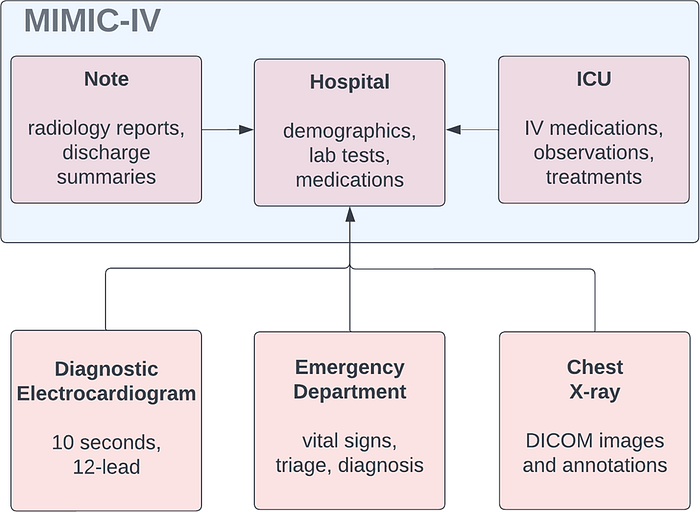
\includegraphics[width=0.6\textwidth]{Images/MIMIC-IV.png}
    \caption{Data sources - MIMIC-IV \cite{johnson2023mimiciv}.}
    \label{fig:data-sources-overview}
\end{figure}

\begin{figure}[t]
    \centering
    
\includegraphics[width=0.6\textwidth]{Images/Empty.png}
    \caption{Structured EHR codes and discharge summaries are extracted from MIMIC-IV, linked at the admission level, and transformed into model-ready inputs for Task~1 (current-visit prediction) and Task~2 (history-aware next-visit prediction).}
    \label{fig:data-sources-overview}
\end{figure}

% ============================================================

\section{Data Preprocessing, Cohort Construction, and Cohort Analysis}
\label{sec:preprocessing}

This section describes how raw MIMIC-IV records are transformed into model-ready multimodal inputs, and characterises the resulting cohort and label space. The pipeline has three stages: (i) preprocessing structured clinical events (diagnoses, procedures, medications, labs), (ii) preprocessing discharge summary text via section parsing and leakage-aware filtering, and (iii) constructing task-specific samples for Task~1 (current-visit) and Task~2 (history-aware next-visit). We then analyse the ICD-9 label distribution (head--tail structure), split coverage, and admission-level multimorbidity, which jointly motivate the evaluation design and the knowledge-augmented TextGen variants in Chapter~\ref{sec:results}.

% \begin{figure}[t]
%     \centering
%     \begin{tikzpicture}[
%         box/.style={draw, rounded corners, align=center, inner sep=6pt, minimum width=0.24\textwidth},
%         arrow/.style={-{Latex[length=2mm]}, thick},
%         node distance=10mm
%     ]
%         \node[box] (raw) {Raw MIMIC-IV\\(hosp/icu + note)};
%         \node[box, right=12mm of raw] (struct) {Structured events\\ICD / procedures\\meds / labs};
%         \node[box, below=8mm of struct] (text) {Discharge summary\\section parsing};

%         \node[box, right=12mm of struct] (merge) {Admission-level\\multimodal record\\(\texttt{subject\_id}, \texttt{hadm\_id})};

%         \node[box, right=12mm of merge] (task1) {Task 1 samples\\(single admission)};
%         \node[box, below=8mm of task1] (task2) {Task 2 samples\\(history $\rightarrow$ next visit)};

%         \draw[arrow] (raw) -- (struct);
%         \draw[arrow] (raw) |- (text);
%         \draw[arrow] (struct) -- (merge);
%         \draw[arrow] (text) -- (merge);
%         \draw[arrow] (merge) -- (task1);
%         \draw[arrow] (merge) |- (task2);
%     \end{tikzpicture}
%     \caption{Preprocessing and cohort construction pipeline. Structured events and discharge summaries are processed independently and merged at the admission level before forming task-specific samples.}
%     \label{fig:preprocessing-pipeline}
% \end{figure}

% ============================================================
\subsection{Structured Clinical Events: Mapping, Early-Course Filtering, and Pruning}
\label{subsec:struct-preproc}

We construct a symbolic representation of each admission from diagnoses, procedures, medications, and laboratory events. The goal is to (i) reduce coding granularity and sparsity, and (ii) obtain a stable vocabulary that supports learning and KG alignment.

\paragraph{Diagnoses (ICD filtering).}
Diagnosis codes are extracted from \texttt{diagnoses\_icd} and filtered by ICD version (ICD-9 in this thesis unless stated otherwise). Codes are de-duplicated and later aggregated per admission.

\paragraph{Procedures (ICD filtering and normalisation).}
Procedure codes are extracted from \texttt{procedures\_icd} and filtered by ICD version. For disambiguation from diagnosis codes and to maintain a uniform token namespace, procedure codes are prefixed with \texttt{PRO\_} (e.g., \texttt{PRO\_36xx}). Codes are de-duplicated and later aggregated per admission.

\paragraph{Medication mapping and early-course proxy.}
Medication orders in MIMIC-IV are indexed by National Drug Codes (NDC), which are overly granular and manufacturer-specific. We map NDC to the Anatomical Therapeutic Chemical hierarchy using RxNorm intermediaries~\cite{nlm_rxnorm} and retain \textbf{ATC level-4 (ATC4)} codes for modelling. 
To reduce outcome-proximal prescribing (e.g., discharge-time medications), we retain medications at the \textbf{earliest recorded prescription timestamp per admission} (i.e., the first observed \texttt{starttime} for each \texttt{(subject\_id, hadm\_id)}). This acts as a conservative proxy for the ``initial treatment context'' without incorporating later-course medication patterns.

\paragraph{Laboratory discretisation.}
Laboratory events are extracted from \texttt{labevents} and converted into symbolic tokens. Concretely, for each patient and lab test (\texttt{itemid}), we retain the \textbf{first recorded value} (patient-level first occurrence) and discretise numeric values into $n=5$ quantile bins, yielding categorical lab symbols of the form \texttt{itemid-value\_bin}. These lab symbols are subsequently aggregated at the admission level when constructing the final cohort.

\paragraph{Vocabulary pruning (long-tail control).}
Clinical code systems are heavy-tailed: a small subset occurs very frequently, while many codes appear rarely. Extremely low-frequency labels provide insufficient support for stable representations and add noise in both neural and graph-based components. We therefore apply frequency-based pruning \emph{before multimodal merging and before splitting}. Specifically, we compute frequencies on the full structured tables and retain:
\begin{itemize}
    \item \textbf{Diagnoses:} Top \textbf{2000} most frequent ICD-9 diagnosis codes.
    \item \textbf{Procedures:} Top \textbf{800} most frequent procedure codes.
    \item \textbf{Labs:} Top \textbf{1500} most frequent discretised lab symbols.
\end{itemize}

\begin{figure}[t]
    \centering
    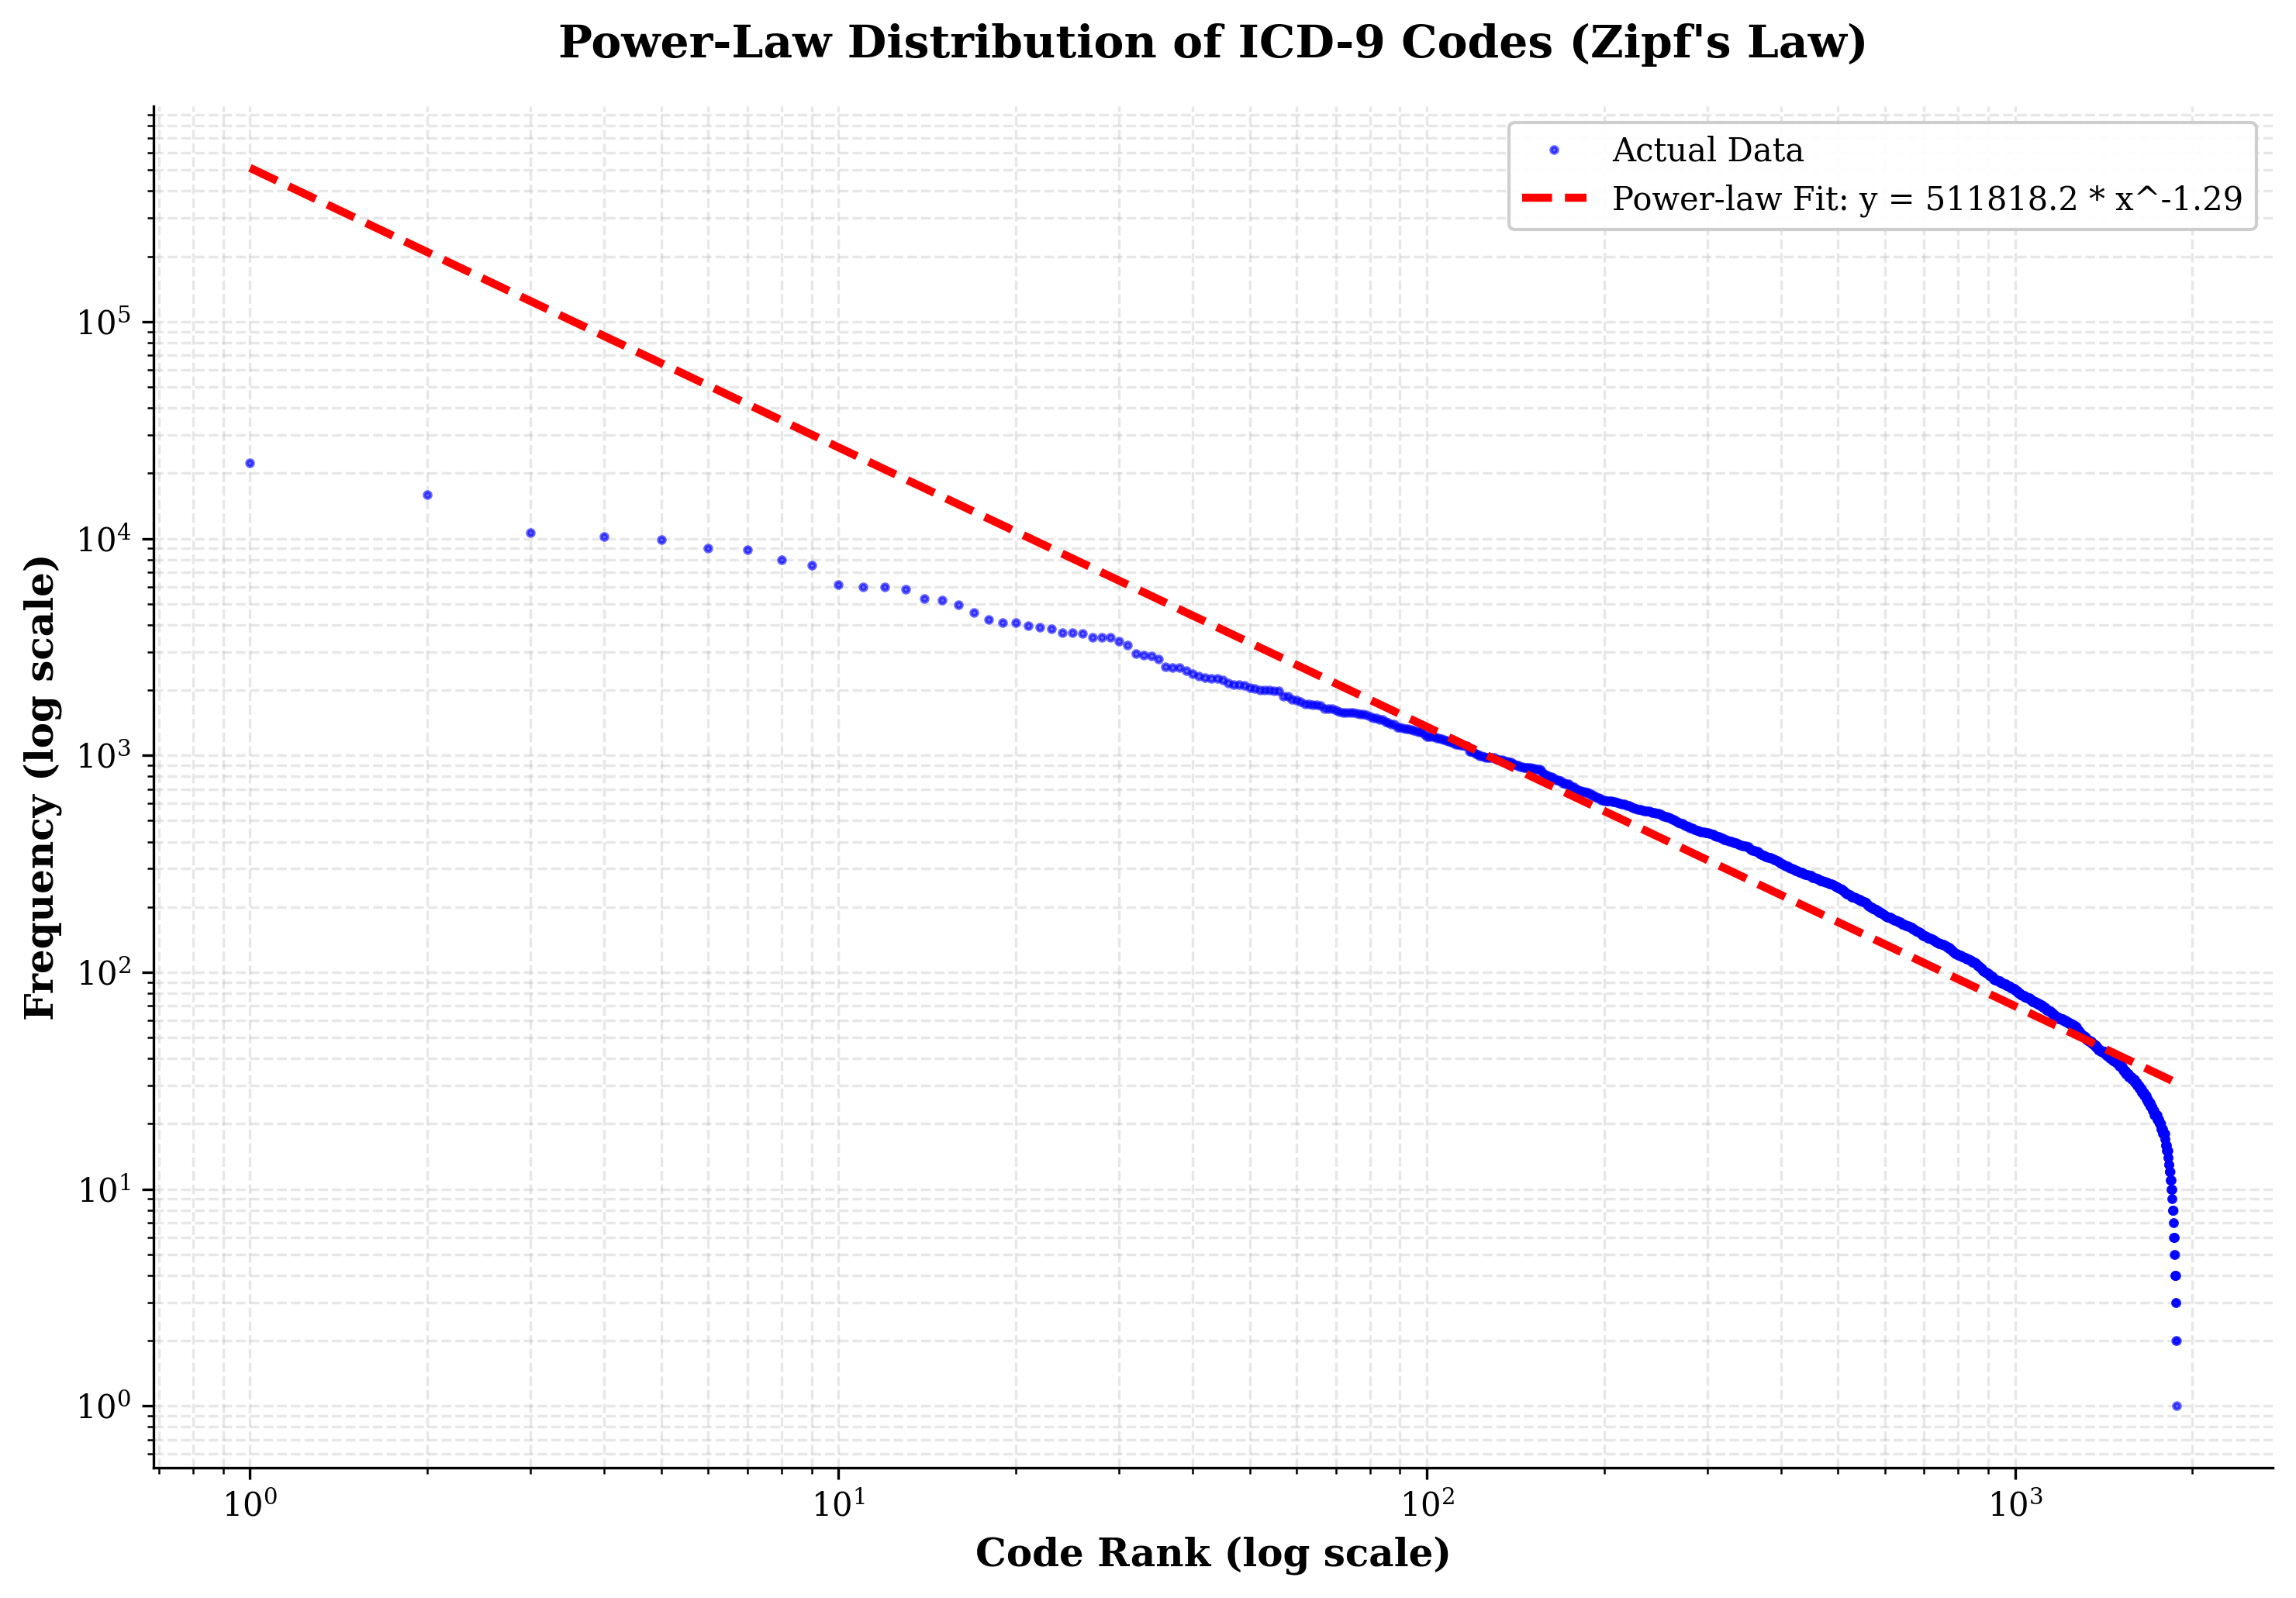
\includegraphics[width=0.8\textwidth]{Images/thesis_plots/power_law_distribution.png}
    \caption{Power-law distribution of global ICD-9 diagnosis frequencies on a log--log scale, together with a fitted trend. The near-linear behaviour confirms a heavy-tailed, Zipf-like structure.}
    \label{fig:diag-power-law}
\end{figure}

% ============================================================
\subsection{Unstructured Text: Discharge Summary Parsing and Leakage Control}
\label{subsec:text-preproc}

Discharge summaries contain heterogeneous formatting and administrative noise. We parse notes using a regex-based, section-aware extractor, producing one column per canonical header (e.g., \textit{Chief Complaint}, \textit{History of Present Illness}, etc.).

\paragraph{Section extraction.}
A single regular expression matches predefined section headers and extracts their corresponding text spans. This converts each discharge summary into a structured set of clinically meaningful fields that can be selectively included depending on the prediction timepoint.

\paragraph{Task-specific section selection (leakage-aware).}
Because Task~1 and Task~2 correspond to different temporal settings, we use different section subsets to minimise information leakage:
\begin{itemize}
    \item \textbf{Task~1 (current-visit diagnosis prediction):} we use a broad discharge-summary view and require non-empty text for
    \textit{Chief Complaint, History of Present Illness, Past Medical History, Family History, Physical Exam, Pertinent Results, Brief Hospital Course,} and \textit{Medications on Admission}.
    \item \textbf{Task~2 (prospective next-visit prediction):} we restrict text to information plausibly available at/near admission:
    \textit{Chief Complaint, History of Present Illness, Past Medical History, Family History, Medications on Admission, Physical Exam}.
    We explicitly exclude outcome-proximal sections such as \textit{Pertinent Results, Brief Hospital Course,} and \textit{Discharge Instructions}.
\end{itemize}

% ============================================================
\subsection{Admission-Level Multimodal Records}
\label{subsec:admission-merge}

Structured events and parsed discharge summary text are merged via \texttt{subject\_id} and \texttt{hadm\_id}. Prior to merging, we enforce an \textbf{admission-level intersection} across structured sources: only admissions that are present in \textit{all} required structured tables (diagnoses, procedures, medications, labs, and admissions metadata) are retained. After this intersection, each admission record contains:
(i) symbolic structured codes (ICD diagnoses, procedures, ATC4 medications, lab tests codes) and
(ii) the section-parsed discharge summary text.

% ============================================================
% \subsection{Task-Specific Cohort Construction}
% \label{subsec:cohort-construction}

% \paragraph{Task~1: Current-visit diagnosis prediction.}
% Each admission constitutes one sample. Labels are the admission’s ICD-9 diagnosis codes (restricted to the pruned diagnosis vocabulary). The multimodal input consists of the admission’s structured codes plus the Task~1 discharge-summary section set (Section~\ref{subsec:text-preproc}).

% \paragraph{Task~2: History-aware next-visit diagnosis prediction.}
% Task~2 converts patient trajectories into longitudinal samples. For a patient with visits $(T_0, T_1, \dots, T_n)$, we create prediction pairs
% $(T_0 \rightarrow T_1, \dots, T_{n-1} \rightarrow T_n)$.
% We use a \textbf{Core + Cold-Start} design:
% \begin{itemize}
%     \item \textbf{Core cohort:} patients with $\ge 2$ admissions provide temporal signal.
%     \item \textbf{Cold-start injection:} a random subset of single-visit patients is injected at \textbf{15\%} of the multi-visit cohort size to ensure robustness to empty-history inputs.
% \end{itemize}

% \paragraph{History vs.\ observation decomposition (Task~2 inputs).}
% For each Task~2 sample $(T_{n-1}\rightarrow T_n)$:
% \begin{itemize}
%     \item \textbf{History (risk profile):} deduplicated union of prior diagnoses and procedures across $T_0\dots T_{n-1}$. Medications are included from the immediately preceding visit $T_{n-1}$ only. Labs are excluded from history due to high temporal variance.
%     \item \textbf{Current observation:} prospective note sections from the current visit $T_n$ (Section~\ref{subsec:text-preproc}).
% \end{itemize}

% % ============================================================
% \subsection{Cohort Statistics and Splits}
% \label{subsec:splits-stats}

% All splits are performed at the \textbf{subject level} to prevent patient-level leakage: all admissions of a subject are assigned exclusively to Train, Validation, or Test. Table~\ref{tab:cohort_stats_task1} summarises Task~1 cohort statistics (to be filled from preprocessing outputs), and Table~\ref{tab:dataset_stats_task2} reports Task~2 cohort composition.

% \begin{table}[t]
% \centering
% \caption{Task~1 cohort statistics after multimodal construction and filtering.}
% \label{tab:cohort_stats_task1}
% \begin{tabular}{ll}
% \toprule
% \textbf{Statistic} & \textbf{Value} \\
% \midrule
% Total unique patients & [T1\_PATIENTS] \\
% Total admissions (samples) & [T1\_ADMISSIONS] \\
% Train/Val/Test split & 80/10/10 (subject-level) \\
% \midrule
% Diagnosis vocabulary (ICD-9) & $\approx 2000$ (pruned) \\
% Procedure vocabulary & $\approx 800$ (pruned) \\
% Medication vocabulary (ATC4) & [ATC4\_COUNT] \\
% Lab vocabulary (discretised) & $\approx 1500$ (pruned) \\
% \bottomrule
% \end{tabular}
% \end{table}

% \begin{table}[t]
%     \centering
%     \caption{Task~2 dataset composition statistics.}
%     \label{tab:dataset_stats_task2}
%     \begin{tabular}{lcc}
%         \toprule
%         \textbf{Metric} & \textbf{Count} & \textbf{Percentage} \\
%         \midrule
%         \textbf{Total unique patients} & \textbf{12,351} & \textbf{100\%} \\
%         Multi-visit patients (core) & 10,740 & 87\% \\
%         Single-visit patients (injection) & 1,611 & 13\% \\
%         \midrule
%         \textbf{Total samples (visit pairs)} & \textbf{28,133} & -- \\
%         \bottomrule
%     \end{tabular}
%     \vspace{0.2cm}
%     \footnotesize{\textit{Note: ``Samples'' exceed ``Patients'' because each multi-visit patient yields multiple prediction pairs (e.g., 3 visits $\rightarrow$ 2 samples).}}
% \end{table}

\subsection{Task-Specific Cohort Construction}
\label{subsec:cohort-construction}

\paragraph{Task~1: Current-visit diagnosis prediction.}
Each admission constitutes one sample. The target is the set of ICD-9 diagnosis codes assigned to that admission (restricted to the pruned diagnosis vocabulary). The input is multimodal: (i) structured admission-level codes (diagnoses/procedures/medications/labs as constructed in Section~\ref{subsec:struct-preproc}) and (ii) the Task~1 discharge-summary section set (Section~\ref{subsec:text-preproc}).

\paragraph{Task~2: History-aware diagnosis prediction (longitudinal setting).}
Task~2 evaluates whether models benefit from longitudinal patient context. For a patient with chronologically ordered admissions $(T_0, T_1, \dots, T_n)$, we construct \emph{one sample per admission} $T_k$ ($k=0,\dots,n$), where the label is the diagnosis set at the \emph{current} admission $T_k$ and the input decomposes into:
\begin{itemize}
    \item \textbf{History signal (pooled):} diagnoses are aggregated as a \emph{deduplicated union} over all prior visits $T_0 \dots T_{k-1}$.
    \item \textbf{Last-visit structured context (most recent):} procedures, medications, and lab symbols are taken from the \emph{immediately preceding visit} $T_{k-1}$ only (not pooled), reflecting recency while avoiding long-range noise.
    \item \textbf{Current narrative context:} leakage-controlled discharge summary sections from the \emph{current} visit $T_k$ (Section~\ref{subsec:text-preproc}).
\end{itemize}

\paragraph{Cold-start handling (explicit empty-history case).}
The first admission $T_0$ has no prior visits; therefore, the structured history fields are set to explicit placeholders (e.g., \texttt{NO\_HISTORY}) and the model must rely primarily on the current clinical text signal. This makes robustness to new patients an explicit part of the Task~2 design.

\paragraph{Core + cold-start cohort design.}
To concentrate training signal on longitudinal reasoning while remaining robust in deployment, Task~2 uses a \textbf{Core + Cold-start} construction:
\begin{itemize}
    \item \textbf{Core cohort:} patients with $\ge 2$ admissions provide genuine temporal signal (learning how prior disease burden relates to future diagnoses).
    \item \textbf{Cold-start injection:} a random subset of single-admission patients is injected at \textbf{15\%} of the multi-visit patient count. This explicitly trains the model to handle \emph{empty-history} inputs, which are unavoidable in real-world settings (e.g., new patients or incomplete longitudinal records), reducing brittleness and discouraging hallucinated history.
\end{itemize}
The two cohorts are split independently at the subject level and merged afterwards to preserve the intended ratio across Train/Validation/Test.

\newcommand{\Dx}{\mathrm{Dx}}
\newcommand{\Proc}{\mathrm{Proc}}
\newcommand{\Med}{\mathrm{Med}}
\newcommand{\Lab}{\mathrm{Lab}}
\newcommand{\Text}{\mathrm{Text}}

\begin{figure}[t]
\centering
\setlength{\fboxsep}{8pt}
\fbox{
\begin{minipage}{0.95\textwidth}
\small
\textbf{Task~2 input decomposition for predicting diagnoses at visit $T_k$}\\[2mm]

\rowcolors{2}{gray!8}{white}
\begin{tabular}{p{0.20\textwidth} p{0.78\textwidth}}
\textbf{Pooled history} & $\Dx_{\le k-1}=\bigcup_{i=0}^{k-1}\Dx(T_i)$ (deduplicated union over all prior visits). \\
\textbf{Last-visit context} & $\Proc(T_{k-1}),\Med(T_{k-1}),\Lab(T_{k-1})$ (only the immediately preceding visit). \\
\textbf{Current observation} & $\Text(T_k)$ (current visit note sections; leakage-controlled). \\
\end{tabular}

\vspace{2mm}
\hrule
\vspace{2mm}

\textbf{Timeline example}\\[1mm]
\rowcolors{2}{gray!8}{white}
\begin{tabular}{l|p{0.80\textwidth}}
$T_0$ & \texttt{NO\_HISTORY} for structured fields; use $\Text(T_0)$ only. \\
$T_1$ & pool $\Dx(T_0)$; last-visit $\Proc/\Med/\Lab(T_0)$; use $\Text(T_1)$. \\
$T_2$ & pool $\Dx(T_0)\cup\Dx(T_1)$; last-visit $\Proc/\Med/\Lab(T_1)$; use $\Text(T_2)$. \\
$\vdots$ & $\vdots$ \\
$T_k$ & pool $\bigcup_{i=0}^{k-1}\Dx(T_i)$; last-visit $\Proc/\Med/\Lab(T_{k-1})$; use $\Text(T_k)$. \\
\end{tabular}
\end{minipage}
}
\caption{Task~2 longitudinal input construction. Diagnoses are pooled across all prior visits, while procedures/medications/labs use only the most recent prior visit. Clinical text is taken from the current visit.}
\label{fig:task2-history-decomposition}
\end{figure}


% \subsection{Cohort Statistics and Splits}
\paragraph{Cohort Statistics and Splits}
\label{subsec:splits-stats}

All data splits are performed at the \textbf{subject level} to prevent patient-level leakage i.e. all admissions belonging to a subject are assigned exclusively to Train, Validation, or Test, ensuring no patient overlap b/w these sets mimicking real-world scenario (where test patients are unseen)

\begin{table}[t]
\centering
\caption{Task~1 cohort size and subject-level splits (after multimodal filtering).}
\label{tab:task1_splits}
\begin{tabular}{lrr}
\toprule
\textbf{Split} & \textbf{Admissions (samples)} & \textbf{Unique patients} \\
\midrule
Train & 42{,}888 & 34{,}079 \\
Validation & 5{,}374 & 4{,}260 \\
Test & 5{,}299 & 4{,}260 \\
\midrule
\textbf{Total} & \textbf{53{,}561} & \textbf{42{,}599} \\
\bottomrule
\end{tabular}
\end{table}

\begin{table}[t]
\centering
\caption{Task~2 cohort composition and final subject-level split sizes (Core + Cold-start injection).}
\label{tab:task2_stats_splits}
\begin{tabular}{lrr}
\toprule
\textbf{Component / Split} & \textbf{Samples (admissions)} & \textbf{Unique patients} \\
\midrule
\multicolumn{3}{l}{\textit{Cohort composition}} \\
Multi-visit patients (core, $\ge 2$ admissions) & 26{,}522 & 10{,}740 \\
Single-visit patients (cold-start injection) & 1{,}611 & 1{,}611 \\
\midrule
\textbf{Total Task~2 dataset} & \textbf{28{,}133} & \textbf{12{,}351} \\
\midrule
\multicolumn{3}{l}{\textit{Final subject-level splits (after merging cohorts)}} \\
Train & 22{,}489 & -- \\
Validation & 2{,}837 & -- \\
Test & 2{,}807 & -- \\
\bottomrule
\end{tabular}
\end{table}

% ============================================================
\subsection{Diagnosis Label-Space Characterisation (Head--Tail)}
\label{subsec:head-tail-cohort}

After preprocessing and pruning, the diagnosis label space contains approximately $C \approx 2{,}000$ ICD-9 codes. Let $\mathcal{D}=\{c_1,\dots,c_C\}$. For each code $c\in\mathcal{D}$, we define a \emph{global} admission-level frequency over the constructed cohort:
\begin{equation}
    f_c^{\text{all}} = \#\{\text{admissions (across train, validation, and test) in which } c \text{ appears at least once}\}.
\end{equation}
Sorting codes by $f_c^{\text{all}}$ yields a rank-ordered sequence $\{c_{(1)},\dots,c_{(C)}\}$.

Figures~\ref{fig:diag-power-law} and~\ref{fig:diag-rankplot} visualise the heavy-tailed (Zipf-like) structure: a small number of very common codes dominate the mass, followed by a long tail of rare diagnoses. This motivates reporting frequency-stratified performance (Head-50 vs.\ Tail-50) in Chapter~\ref{sec:results}.

\begin{figure}[t]
    \centering
    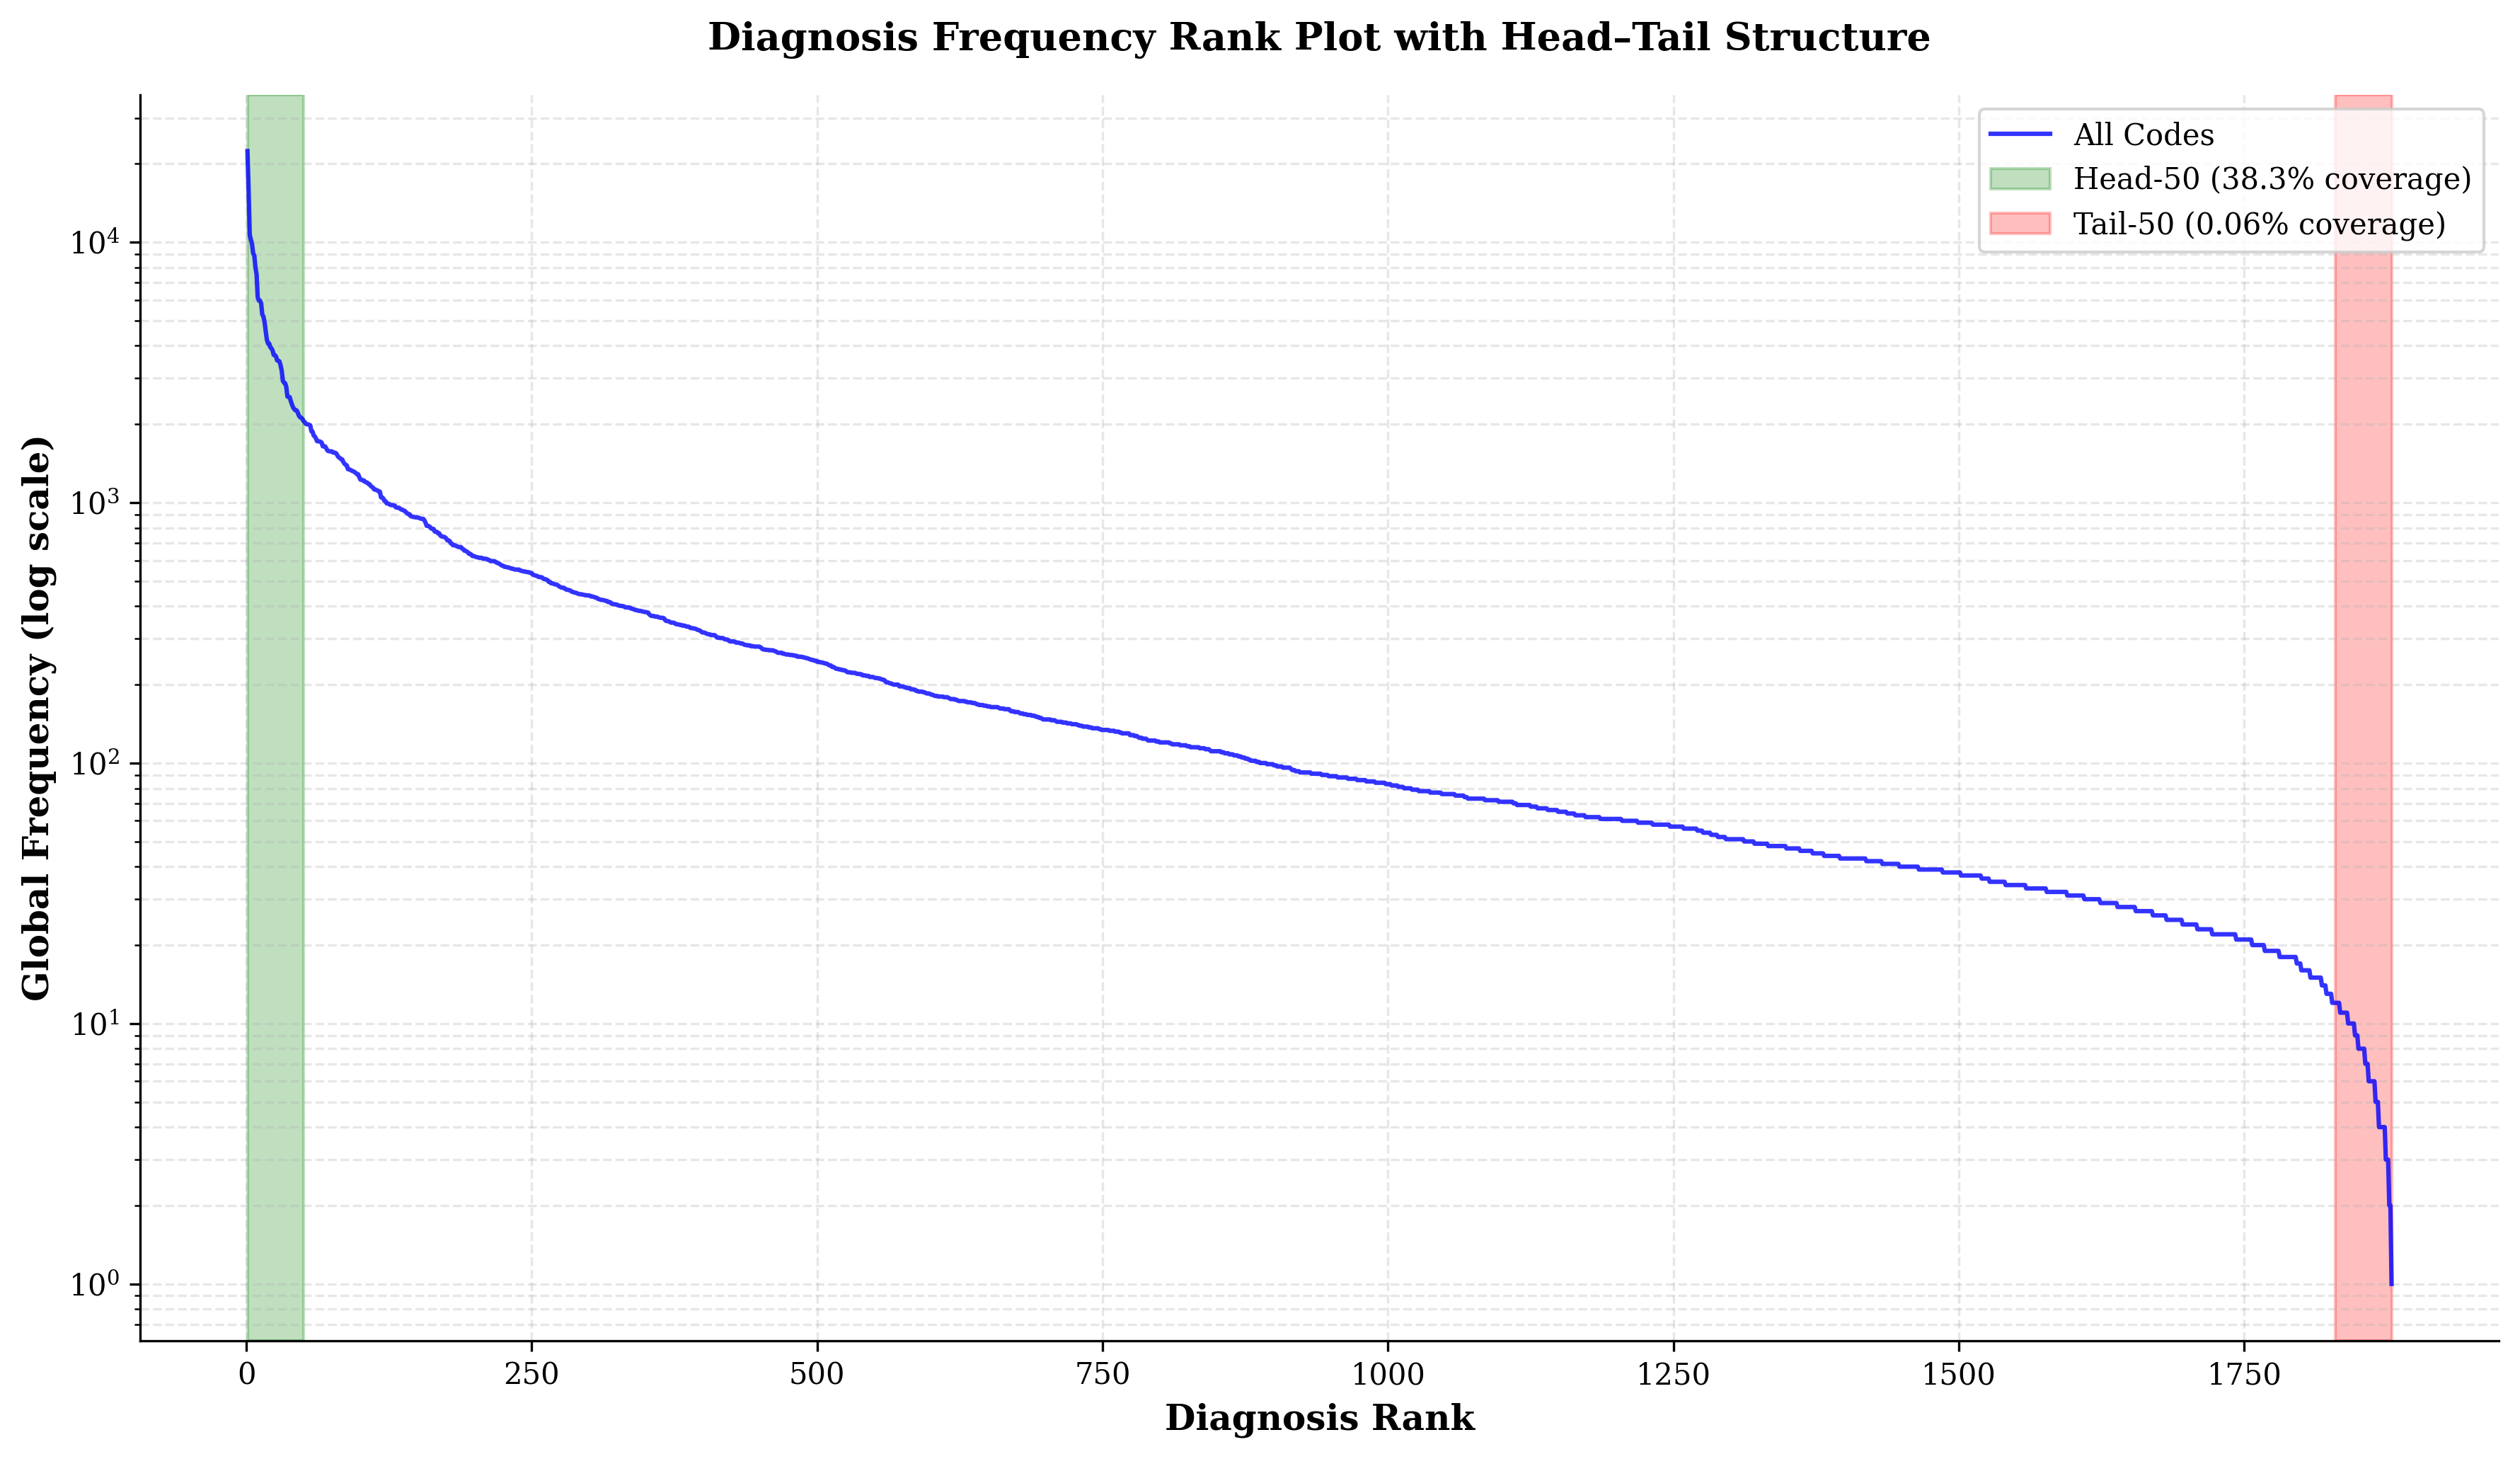
\includegraphics[width=0.8\textwidth]{Images/thesis_plots/diag_frequency_rankplot.png}
    \caption{Global diagnosis frequency rank plot for the retained ICD-9 codes. The green band marks the 50 most frequent codes (\emph{Head-50}), and the red band marks the 50 least frequent codes (\emph{Tail-50}).}
    \label{fig:diag-rankplot}
\end{figure}

We define extremal subsets:
\[
\mathcal{H}_{50}=\{c_{(1)},\dots,c_{(50)}\}, \qquad
\mathcal{T}_{50}=\{c_{(C-49)},\dots,c_{(C)}\}.
\]
Tail codes remain clinically meaningful but are under-represented, making them challenging for data-driven models.

\begin{table}[t]
\centering
\caption{Code frequency categories (Task~1).}
\label{tab:code_freq_1}
\begin{tabular}{lccc}
\toprule
\textbf{Category} & \textbf{Number of Codes} & \textbf{Percentage of Total (\%)} & \textbf{Total Instances} \\
\midrule
Very Common (Top 1\%)     & 19  & 1.01  & 154694 \\
Common (Top 5\%)          & 75  & 3.99  & 161150 \\
Frequent (Top 10\%)       & 94  & 5.00  & 87630  \\
Moderate (Top 25\%)       & 283 & 15.06 & 118378 \\
Uncommon (50--75\%)       & 470 & 25.01 & 73364  \\
Rare (25--50\%)           & 477 & 25.39 & 30434  \\
Very Rare (Bottom 25\%)   & 461 & 24.53 & 12312  \\
\bottomrule
\end{tabular}
\end{table}

\begin{table}[t]
\centering
\caption{Code frequency categories (Task~2).}
\label{tab:code_freq_2}
\begin{tabular}{lccc}
\toprule
\textbf{Category} & \textbf{Number of Codes} & \textbf{Percentage of Total (\%)} & \textbf{Total Instances} \\
\midrule
Very Common (Top 1\%)     & 19  & 1.02  & 90198  \\
Common (Top 5\%)          & 75  & 4.01  & 101524 \\
Frequent (Top 10\%)       & 94  & 5.02  & 53809  \\
Moderate (Top 25\%)       & 281 & 15.02 & 72489  \\
Uncommon (50--75\%)       & 468 & 25.01 & 43776  \\
Rare (25--50\%)           & 491 & 26.24 & 16902  \\
Very Rare (Bottom 25\%)   & 443 & 23.68 & 5009   \\
\bottomrule
\end{tabular}
\end{table}

\begin{figure}[t]
    \centering
    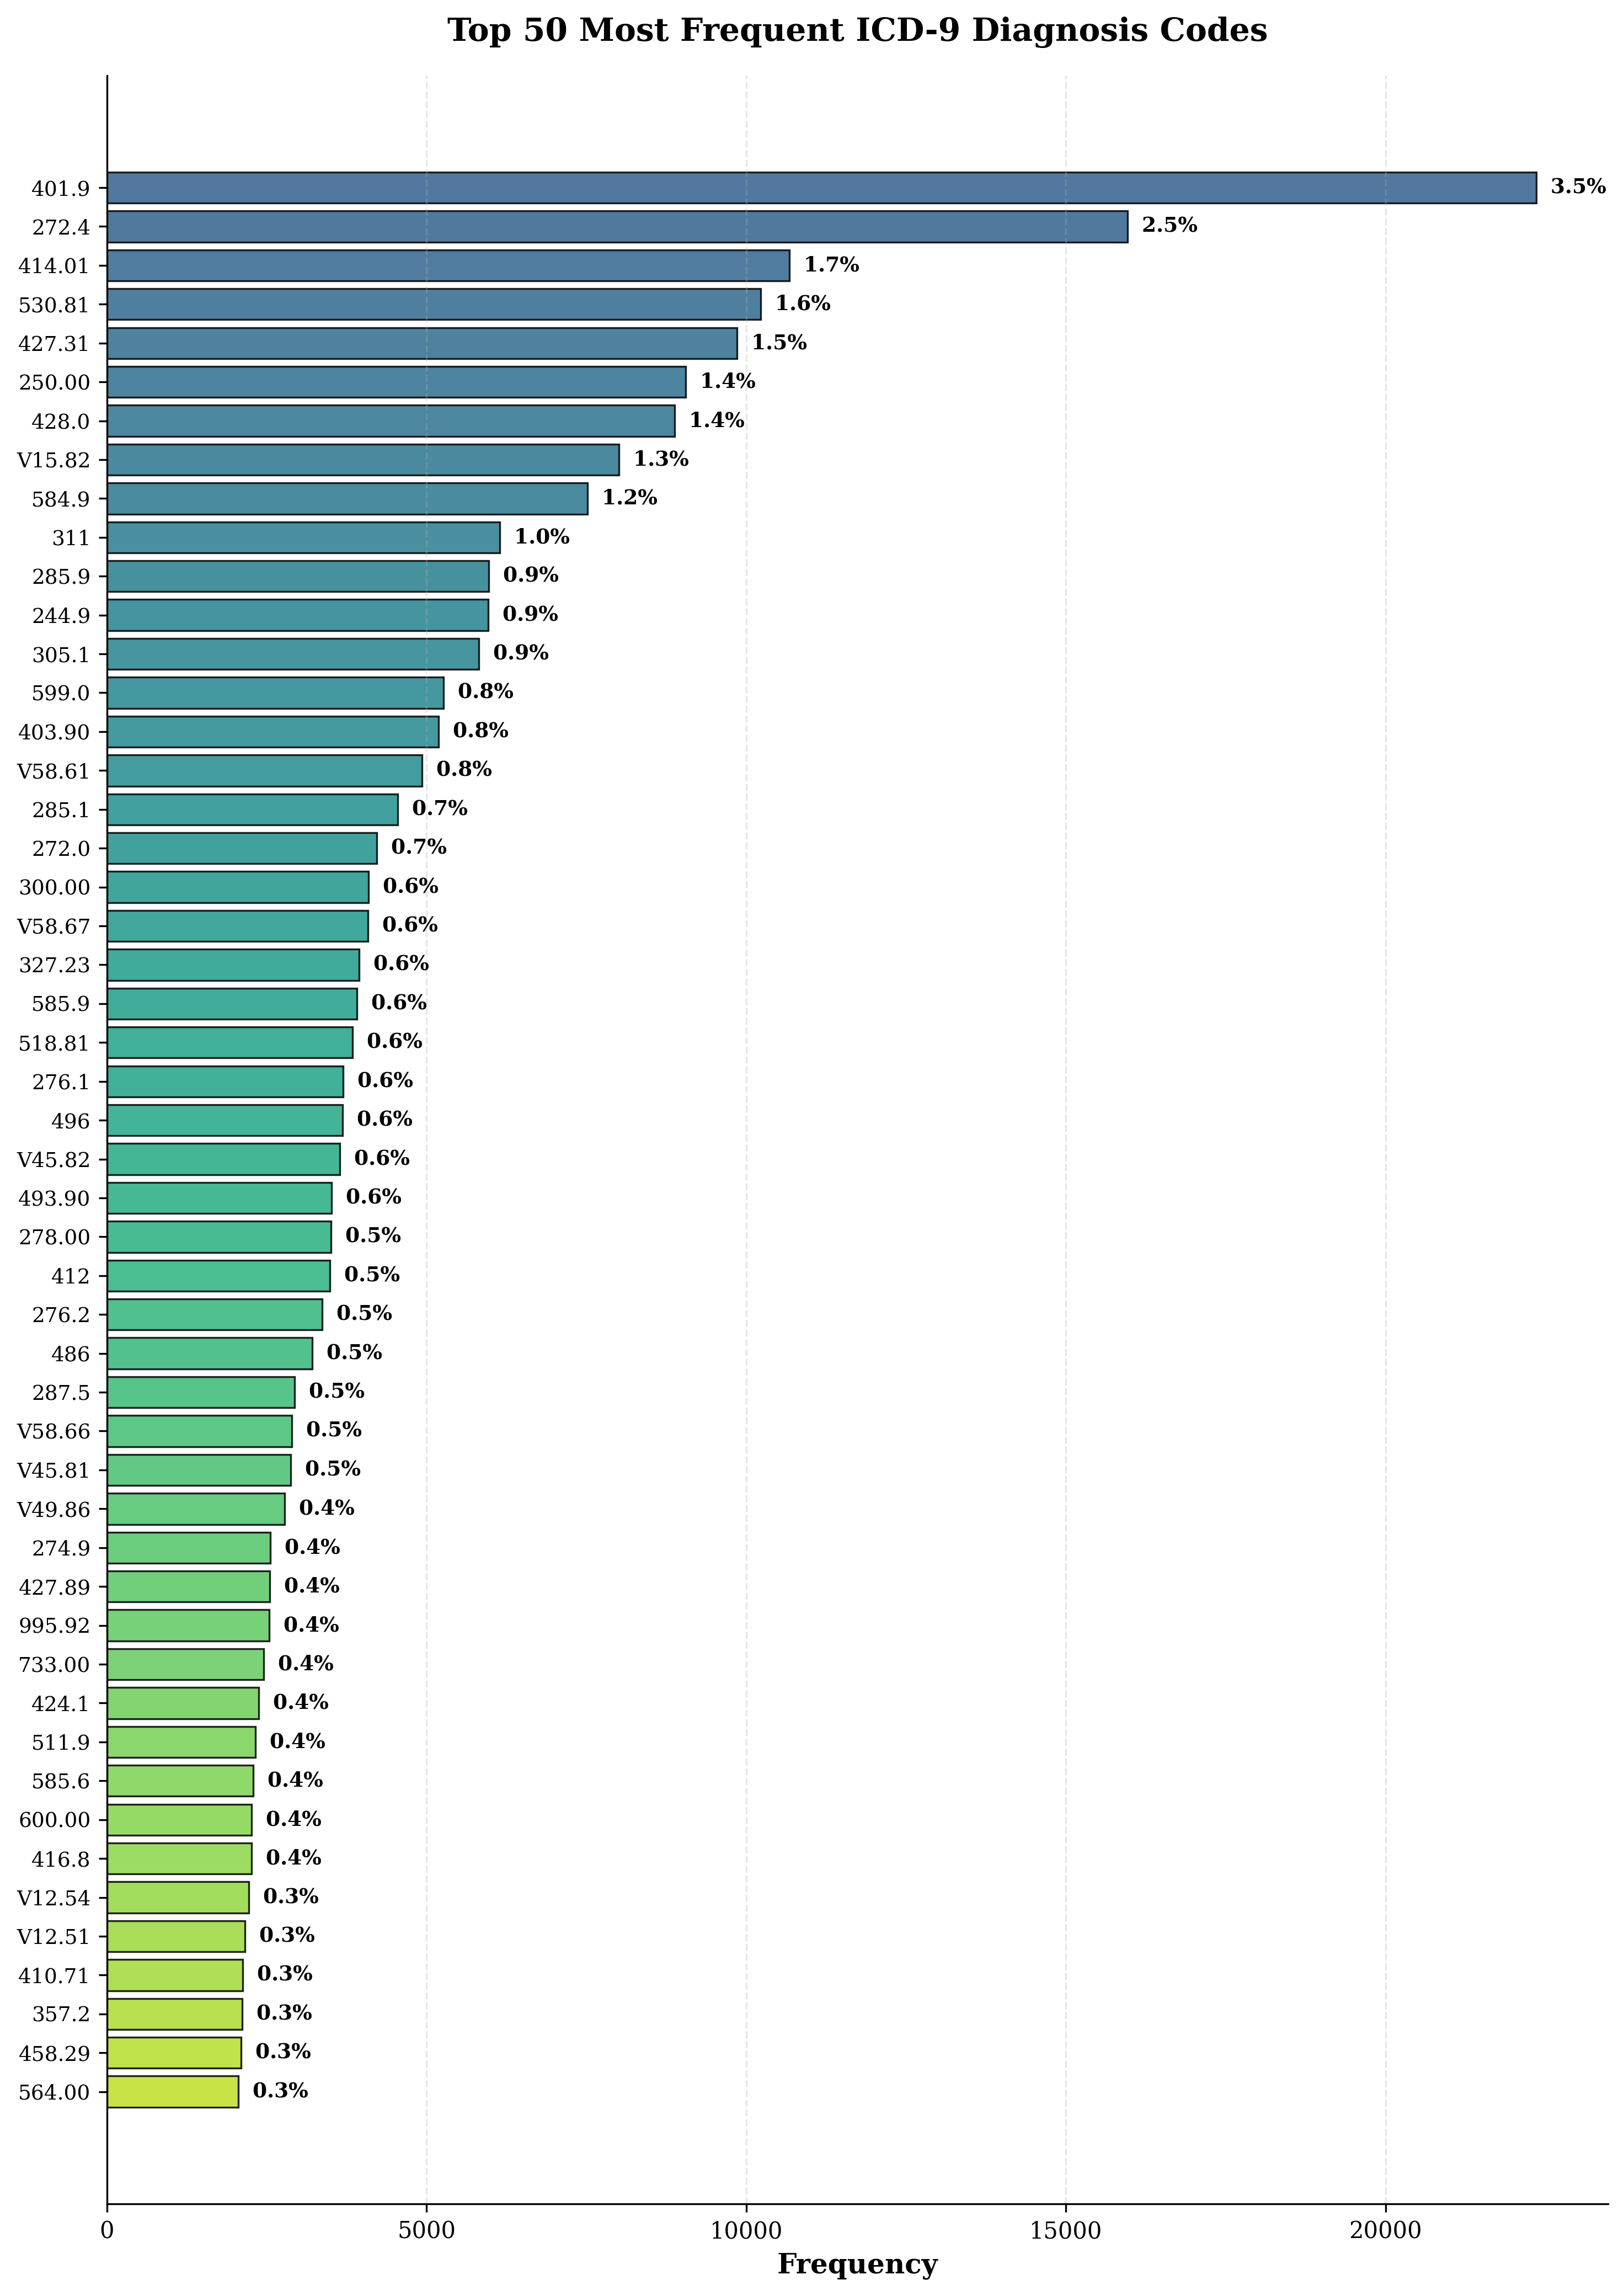
\includegraphics[width=0.8\textwidth]{Images/thesis_plots/top_50_codes_bar.png}
    \caption{Top 50 most frequent ICD-9 diagnosis codes (Head-50) with global frequencies.}
    \label{fig:head50-codes}
\end{figure}

\begin{figure}[t]
    \centering
    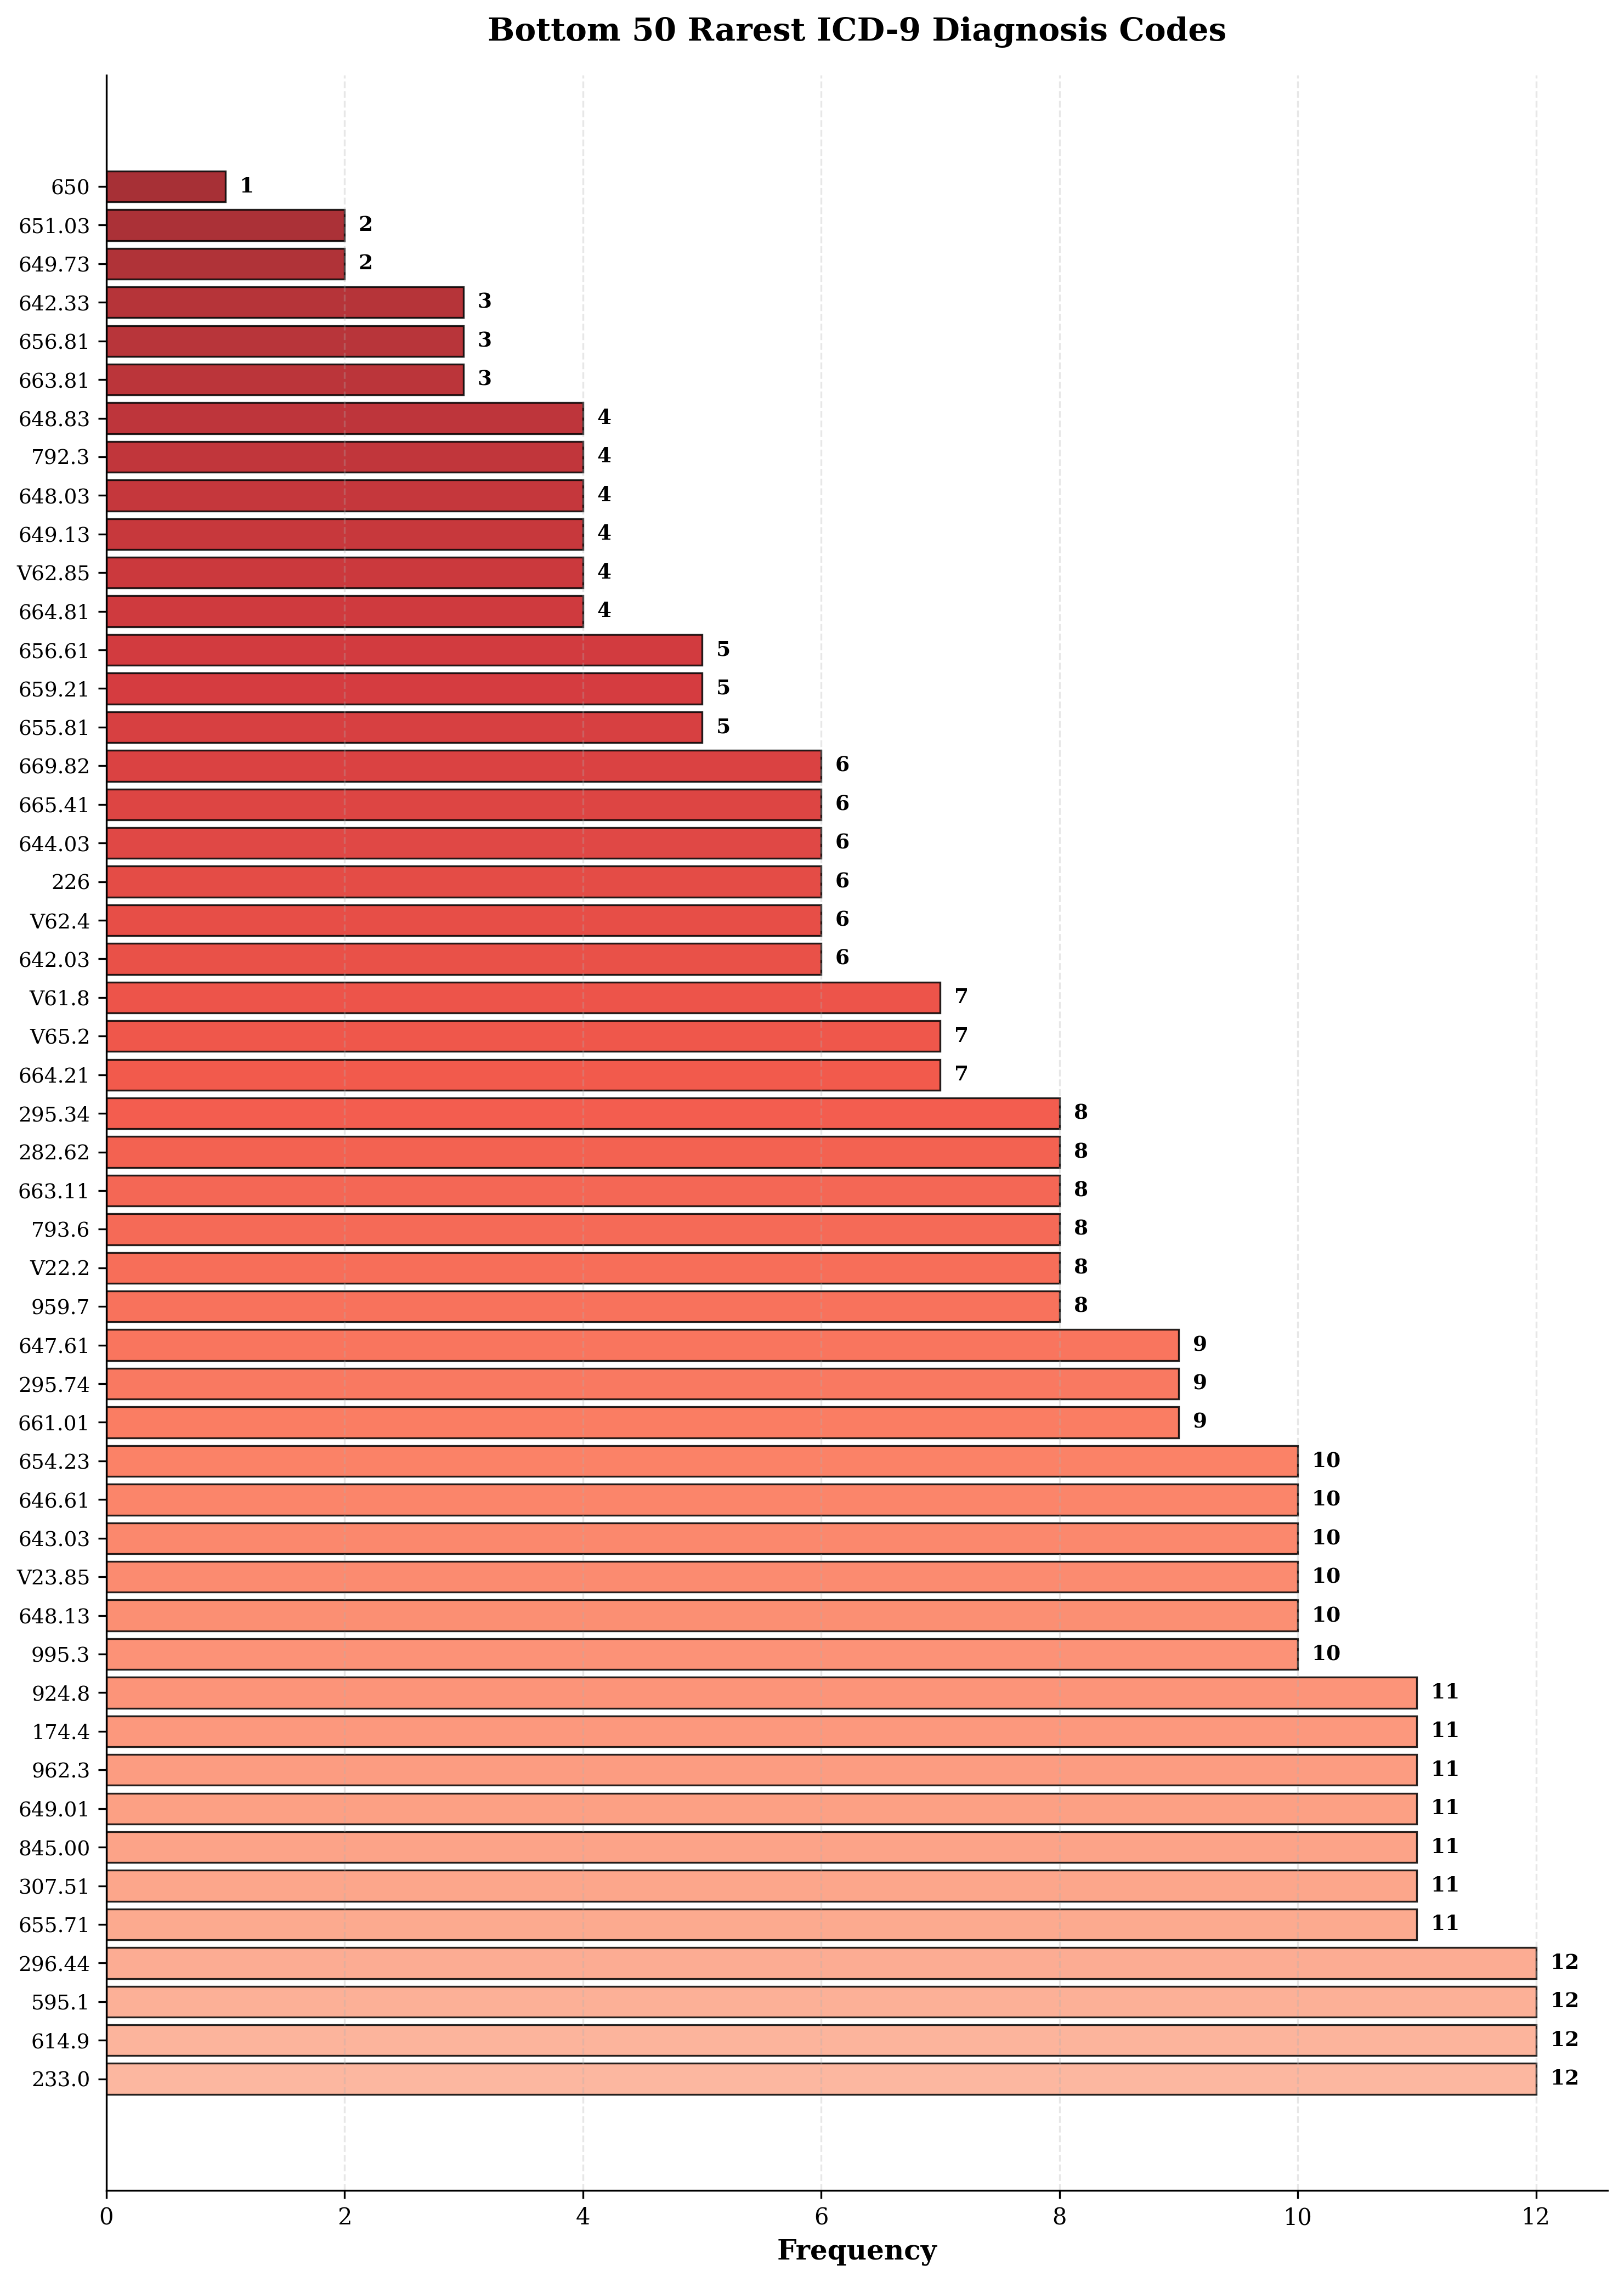
\includegraphics[width=0.8\textwidth]{Images/thesis_plots/bottom_50_codes_bar.png}
    \caption{Bottom 50 rarest ICD-9 diagnosis codes (Tail-50) with global frequencies. Many occur only a handful of times in the dataset.}
    \label{fig:tail50-codes}
\end{figure}

\paragraph{Split coverage and ``zero-shot'' codes.}
We analyse how codes distribute across Train/Validation/Test. Figure~\ref{fig:complete-code-coverage} reports split-level code coverage and a zero-shot check. In this cohort, all test codes are observed in training (0\% zero-shot at the code level), implying that evaluation reflects a \emph{frequency-driven} challenge (rare vs.\ common) rather than unseen-label generalisation.

\begin{figure}[t]
    \centering
    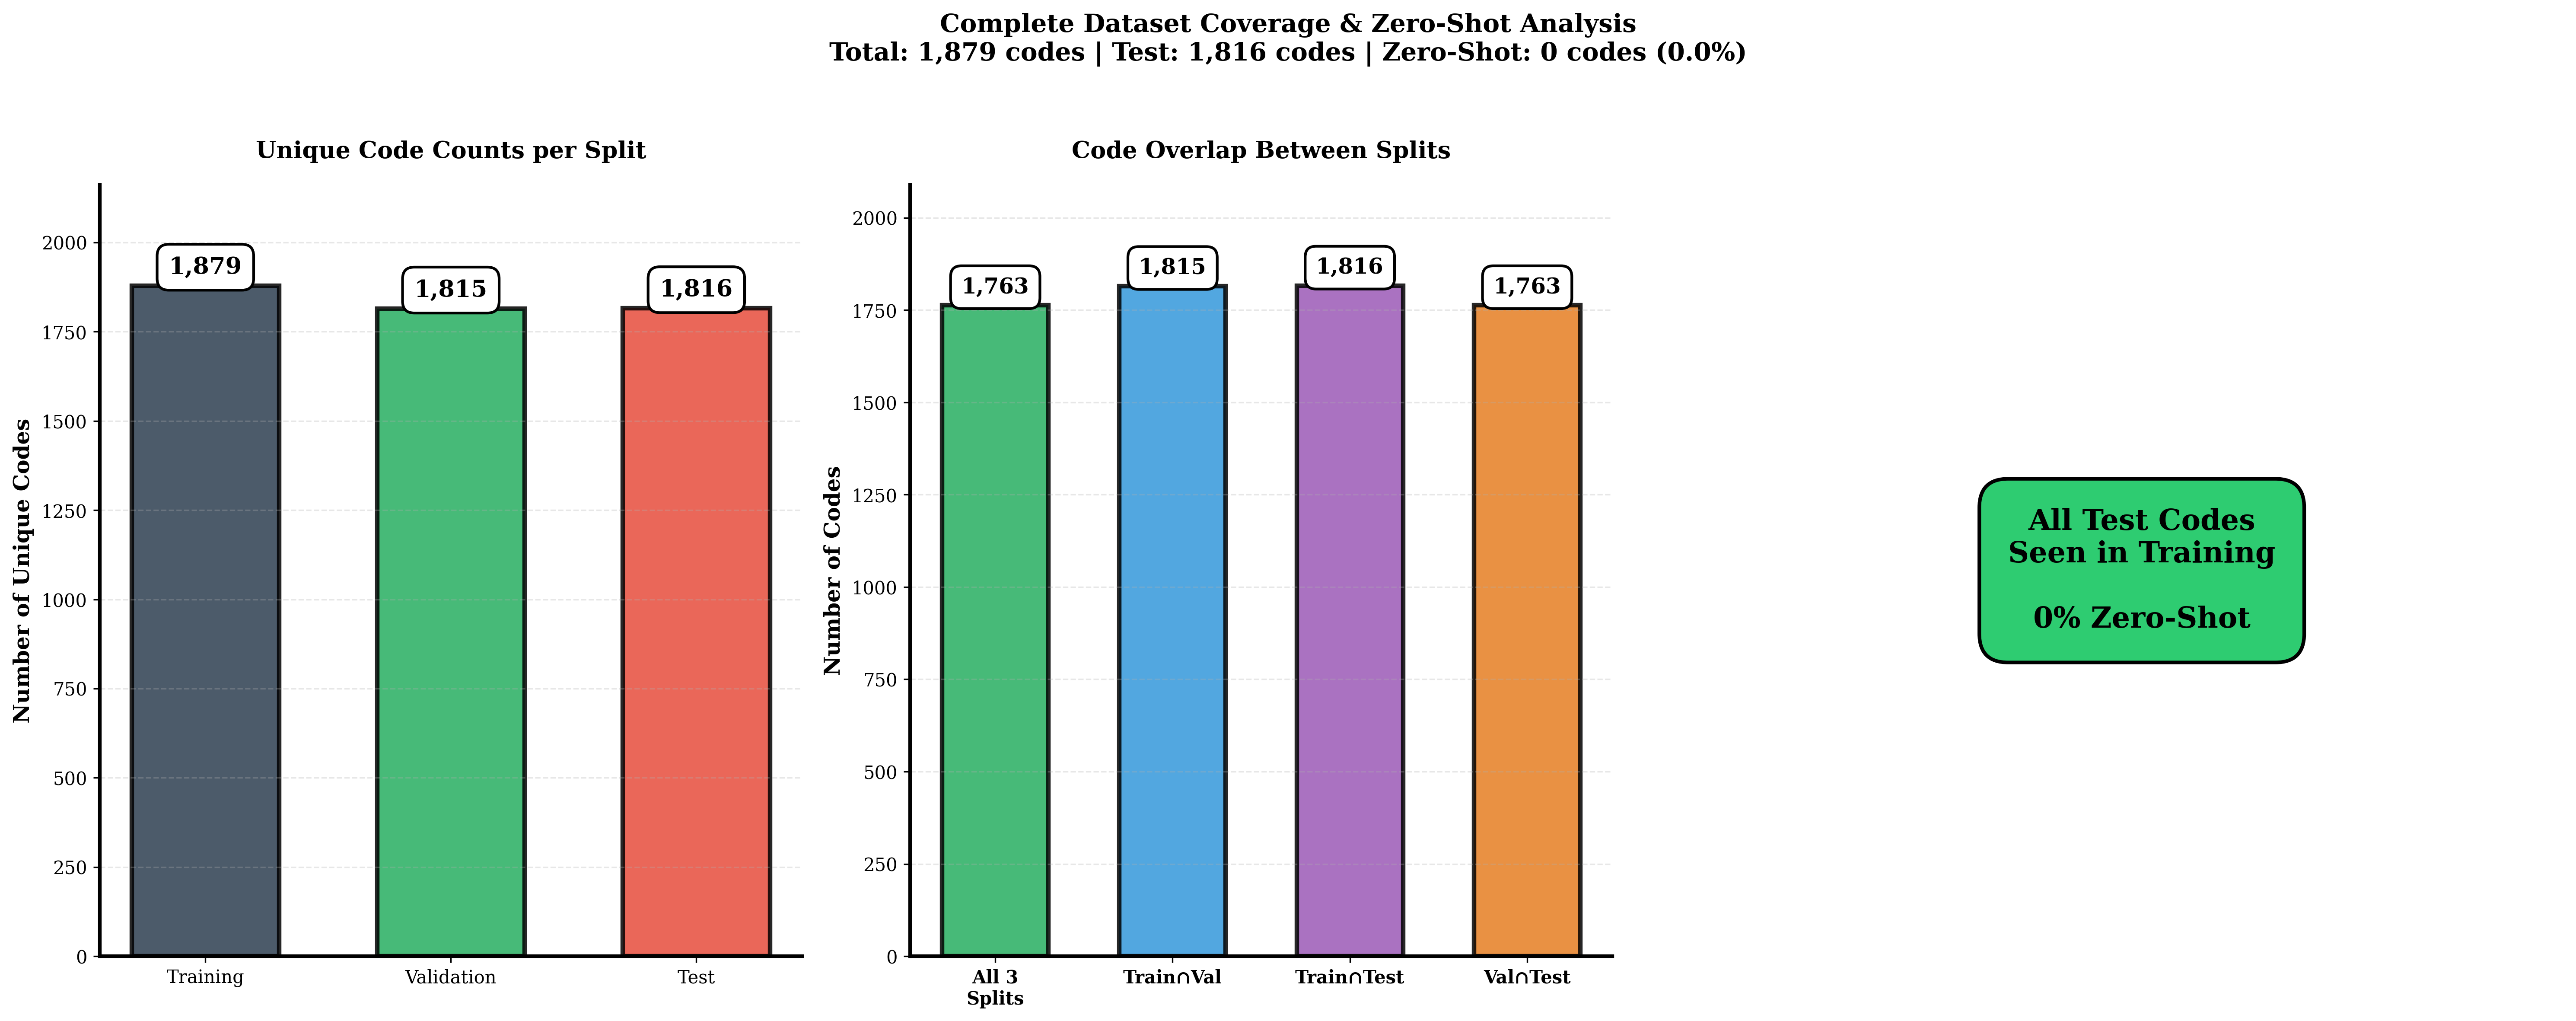
\includegraphics[width=0.95\textwidth]{Images/thesis_plots/complete_code_coverage_zeroshot.png}
    \caption{Complete dataset code coverage and zero-shot analysis. All test codes are seen in training, so evaluation focuses on frequency-driven difficulty rather than unseen-code generalisation.}
    \label{fig:complete-code-coverage}
\end{figure}

\paragraph{Tail-50 evaluation support.}
Because Tail-50 codes are extremely rare, not all globally-defined Tail-50 codes appear in each split. Figure~\ref{fig:global-tail50-presence} illustrates this. Consequently, Tail-50 reporting in Chapter~\ref{sec:results} evaluates on the supported subset $\mathcal{T}_{50}\cap\mathcal{D}_{\text{test}}$ to avoid undefined macro quantities from zero-support labels.

\begin{figure}[t]
    \centering
    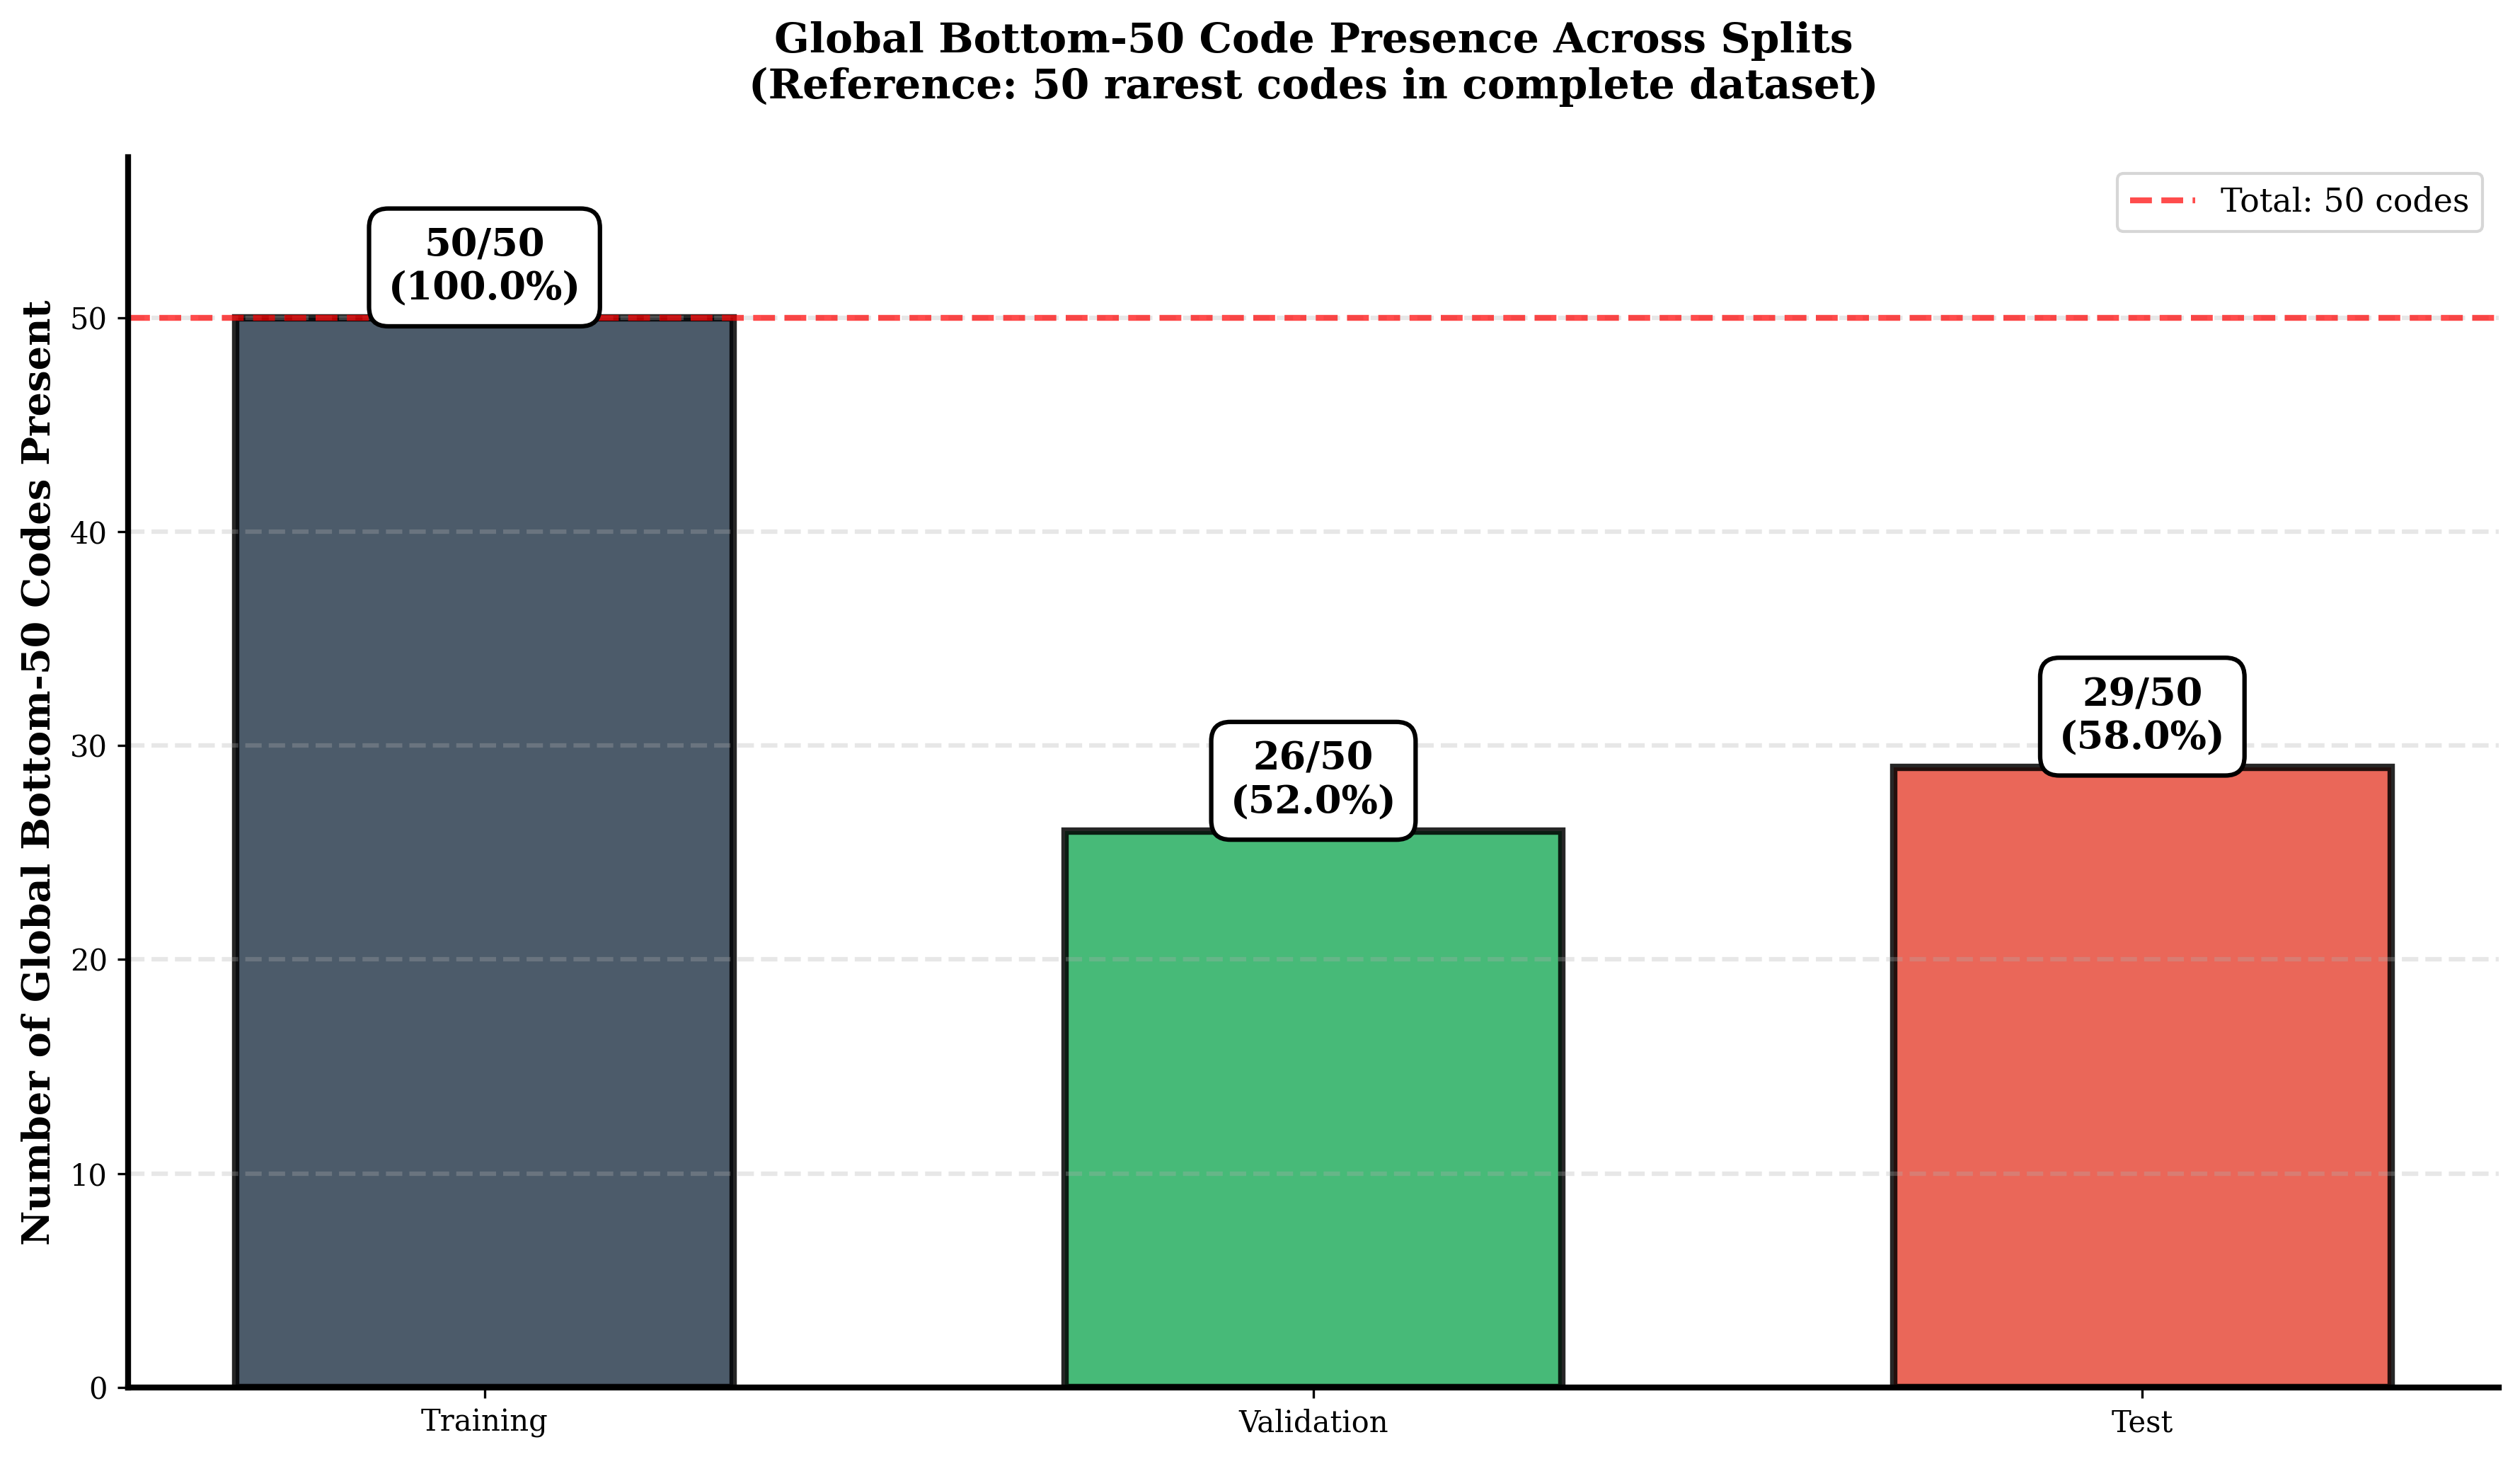
\includegraphics[width=0.85\textwidth]{Images/thesis_plots/global_bottom_50_split_presence.png}
    \caption{Presence of the globally-defined Tail-50 codes across Train/Validation/Test. Only a subset occurs in Validation and Test, motivating Tail-50 evaluation on the Tail-50$\cap$Test intersection.}
    \label{fig:global-tail50-presence}
\end{figure}

% ============================================================
\subsection{ICD-9 Chapters and Parent Categories}
\label{subsec:chapter-cohort}

Beyond individual codes, we characterise higher-level diagnostic themes. Figure~\ref{fig:chapter-distribution} shows the ICD-9 chapter distribution, providing clinically interpretable context for model behaviour. Figure~\ref{fig:top50-parent} aggregates diagnoses at the three-digit parent level and plots the most frequent parent categories. These parent categories are later used for hierarchical evaluation (Section~\ref{subsec:hierarchical-metrics}) and for interpreting clinically tolerant near misses (correct disease family but incorrect subtype).

\begin{figure}[t]
    \centering
    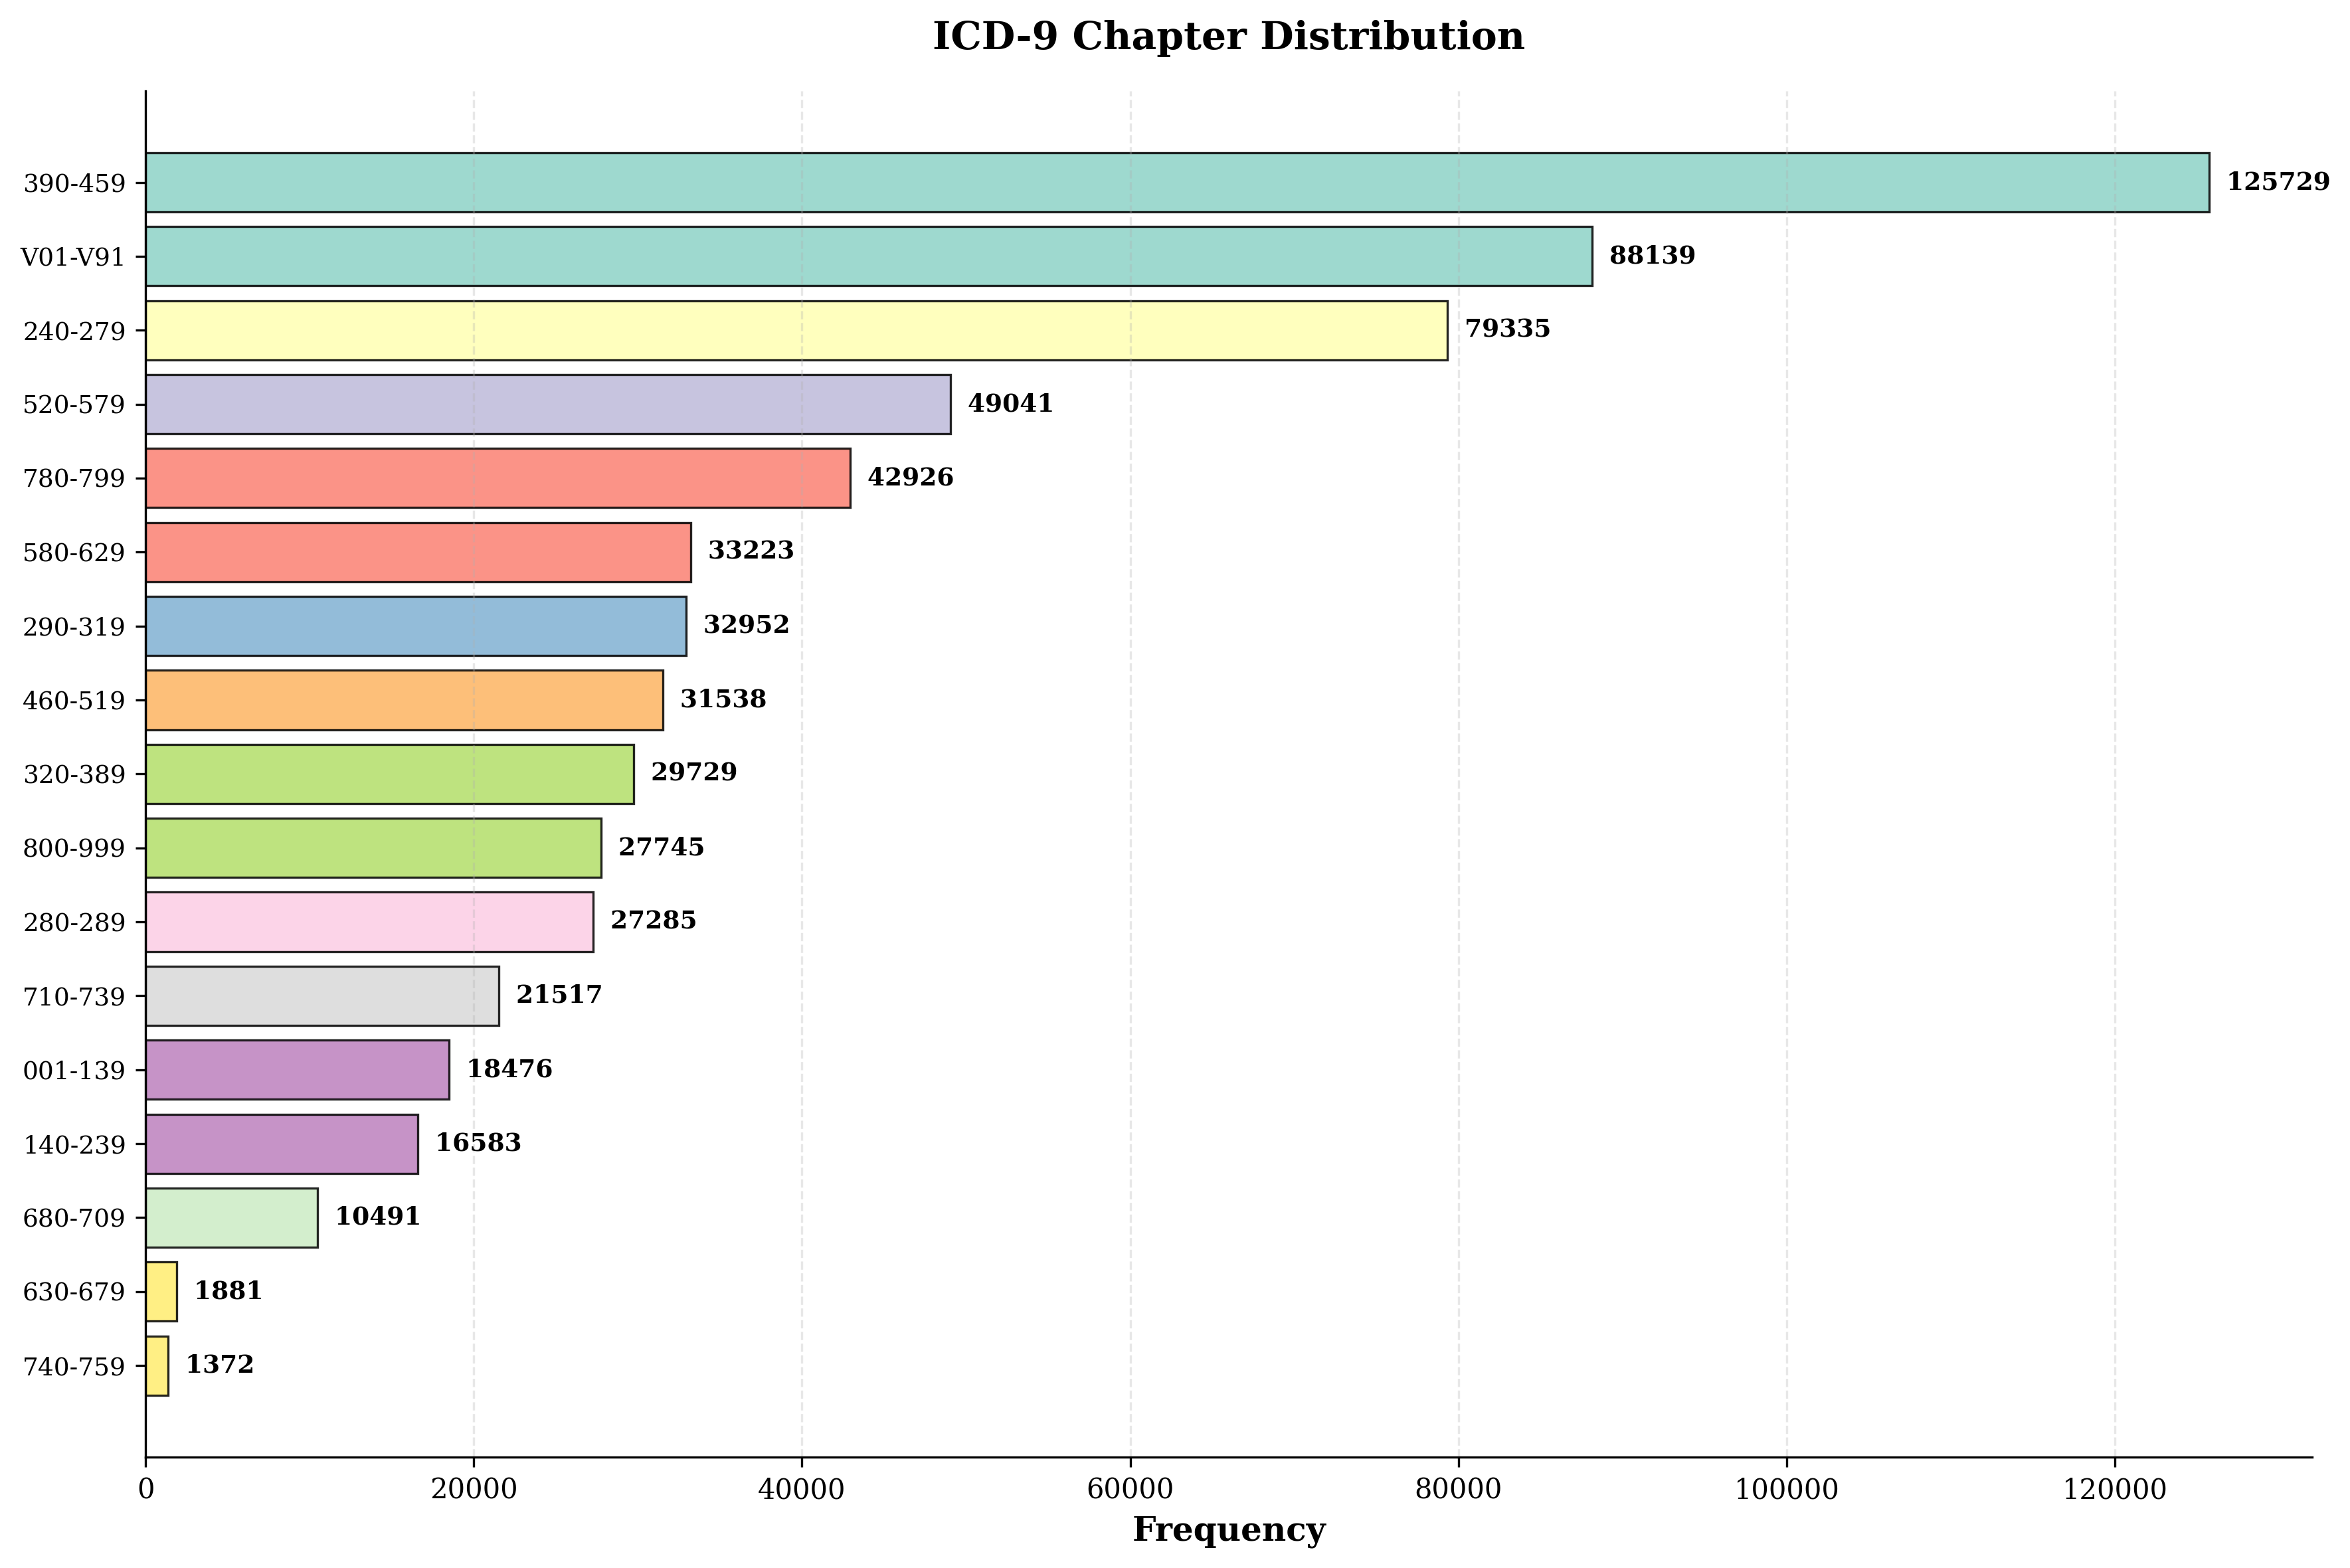
\includegraphics[width=0.9\textwidth]{Images/thesis_plots/chapter_distribution_bar.png}
    \caption{ICD-9 chapter-level distribution based on aggregated frequencies across all codes within each chapter range.}
    \label{fig:chapter-distribution}
\end{figure}

\begin{figure}[t]
    \centering
    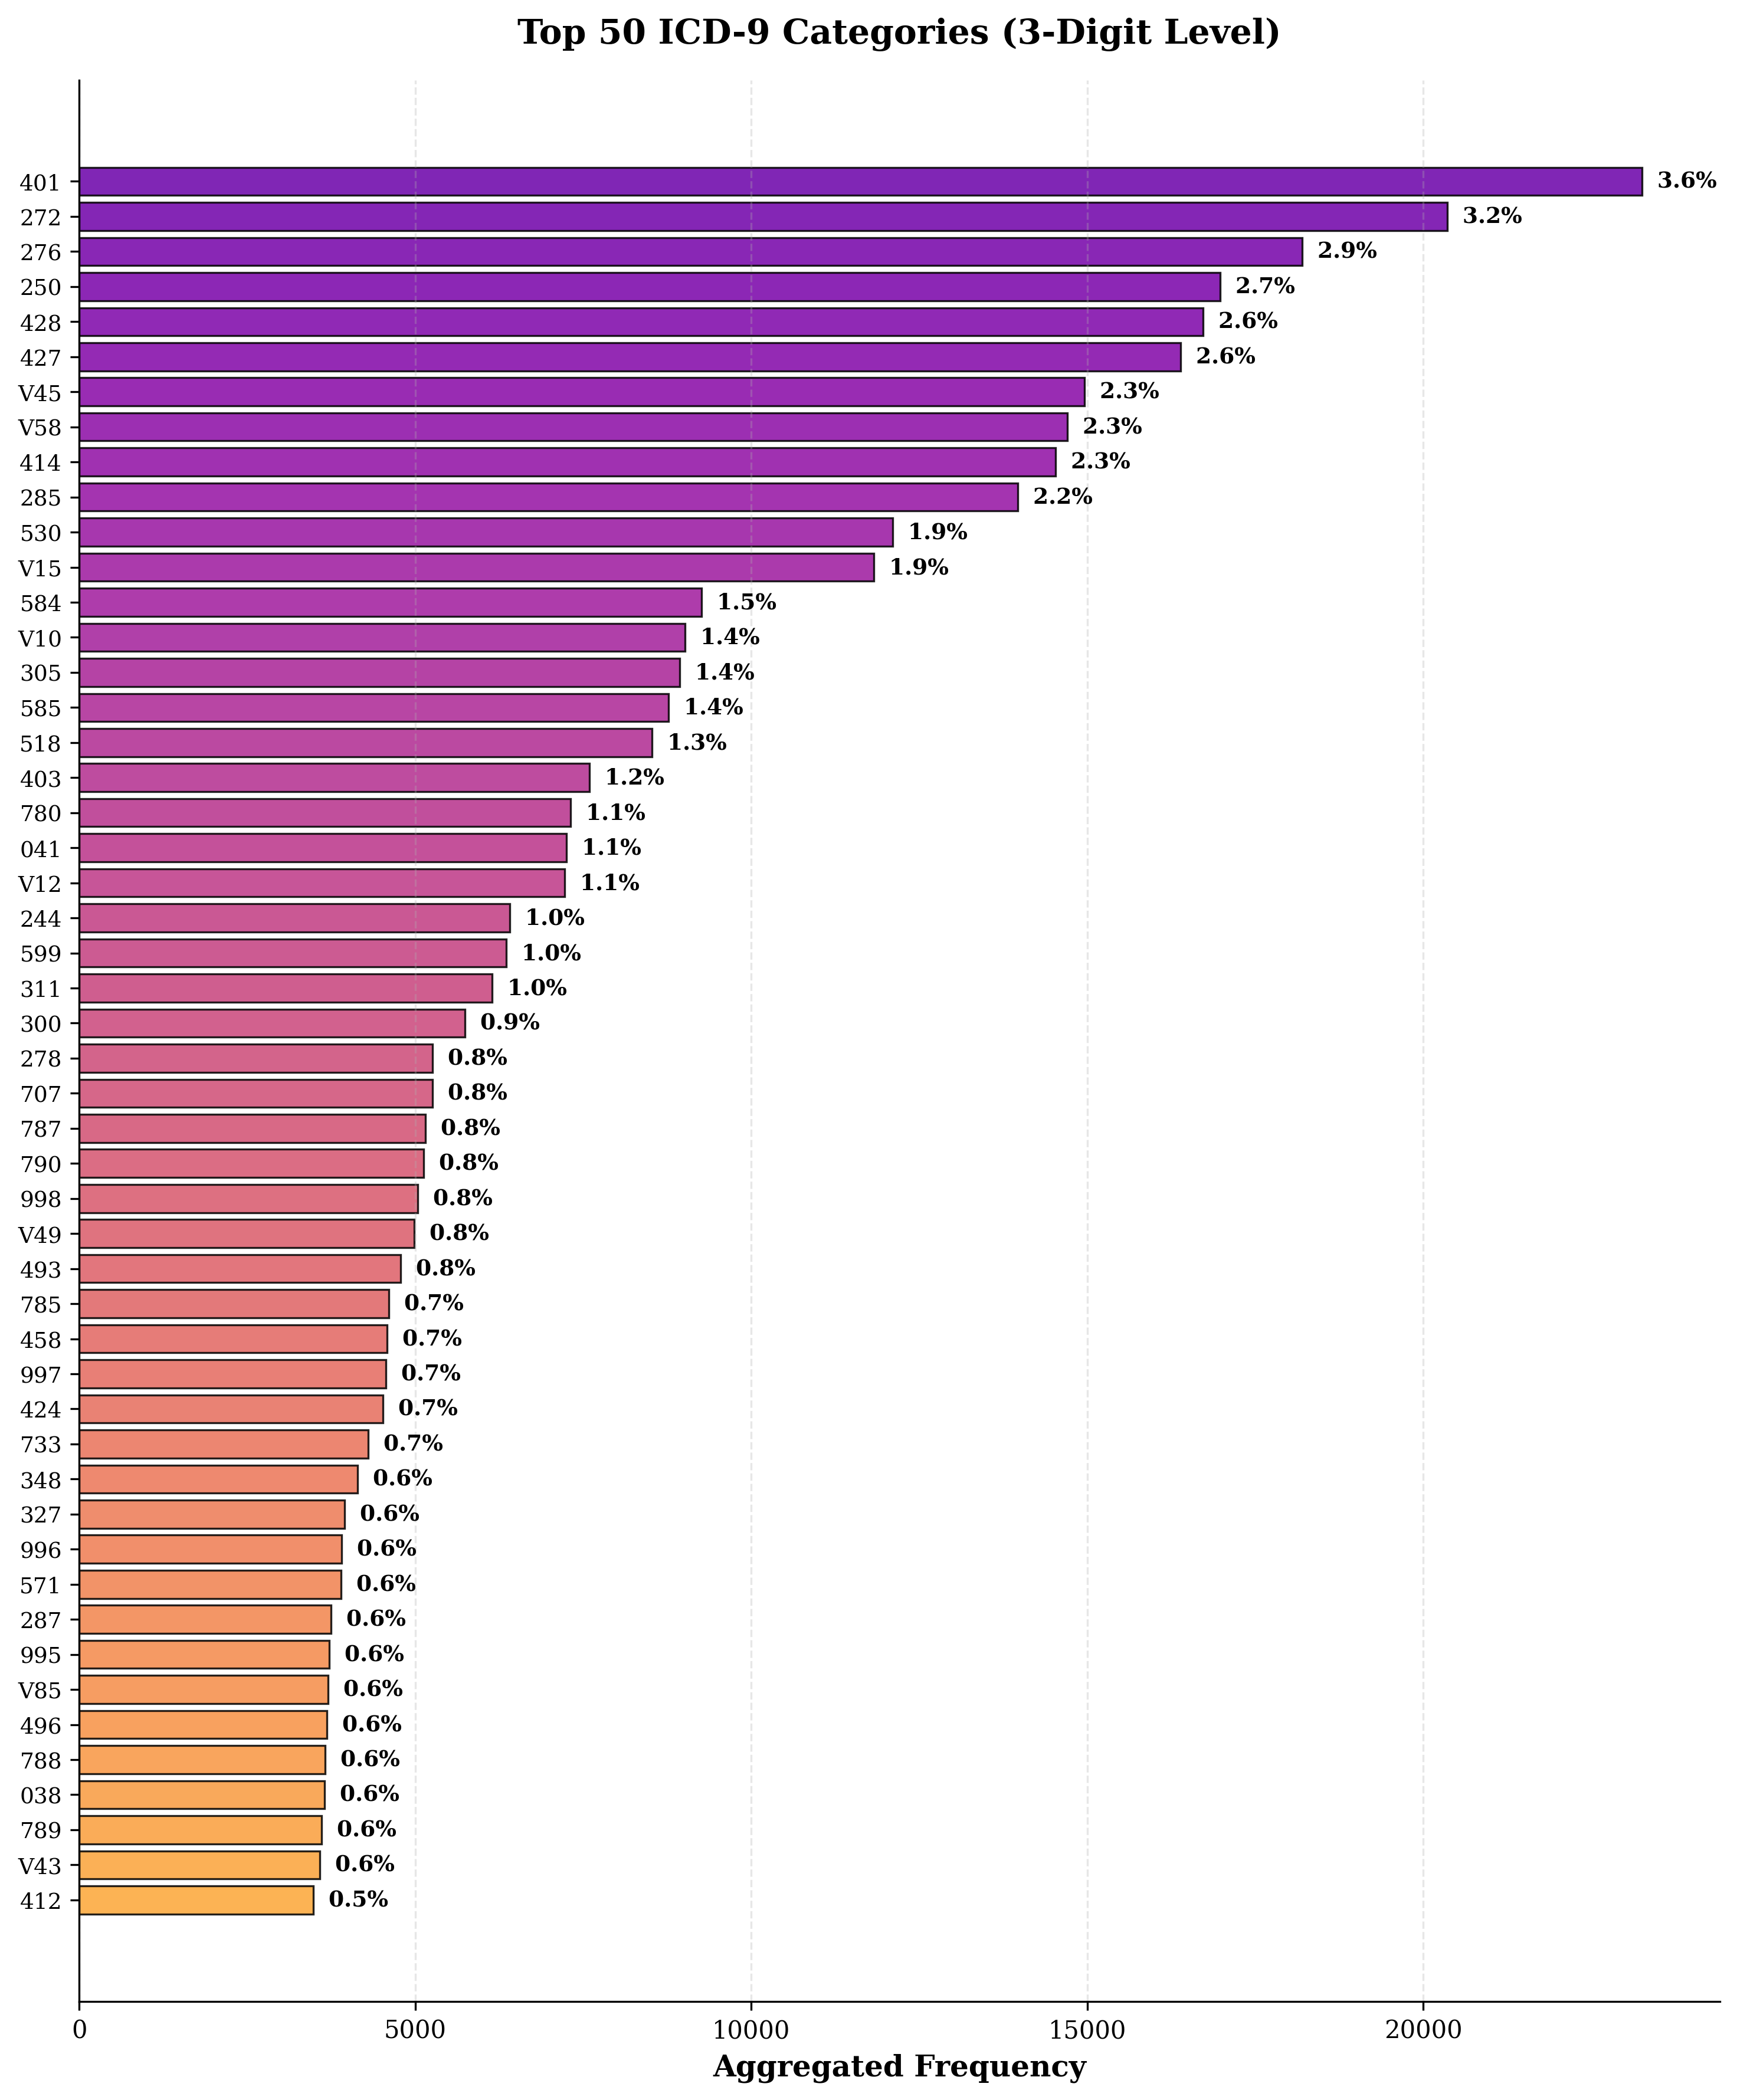
\includegraphics[width=0.8\textwidth]{Images/thesis_plots/top_50_category_levels_bar.png}
    \caption{Top 50 ICD-9 parent categories (three-digit level) by aggregated frequency.}
    \label{fig:top50-parent}
\end{figure}

% ============================================================
\subsection{Multimorbidity and Admission Complexity}
\label{subsec:complexity-cohort}

To quantify clinical complexity, we measure the number of diagnosis codes per admission. For admission $i$, let
\begin{equation}
    L^{(i)} = \#\{c\in\mathcal{D}\mid c \text{ is assigned to admission } i\}
\end{equation}
denote its diagnosis count. Figures~\ref{fig:diag-per-admission-hist} and~\ref{fig:diag-per-admission-box} show the distribution overall and by split.

\begin{figure}[t]
    \centering
    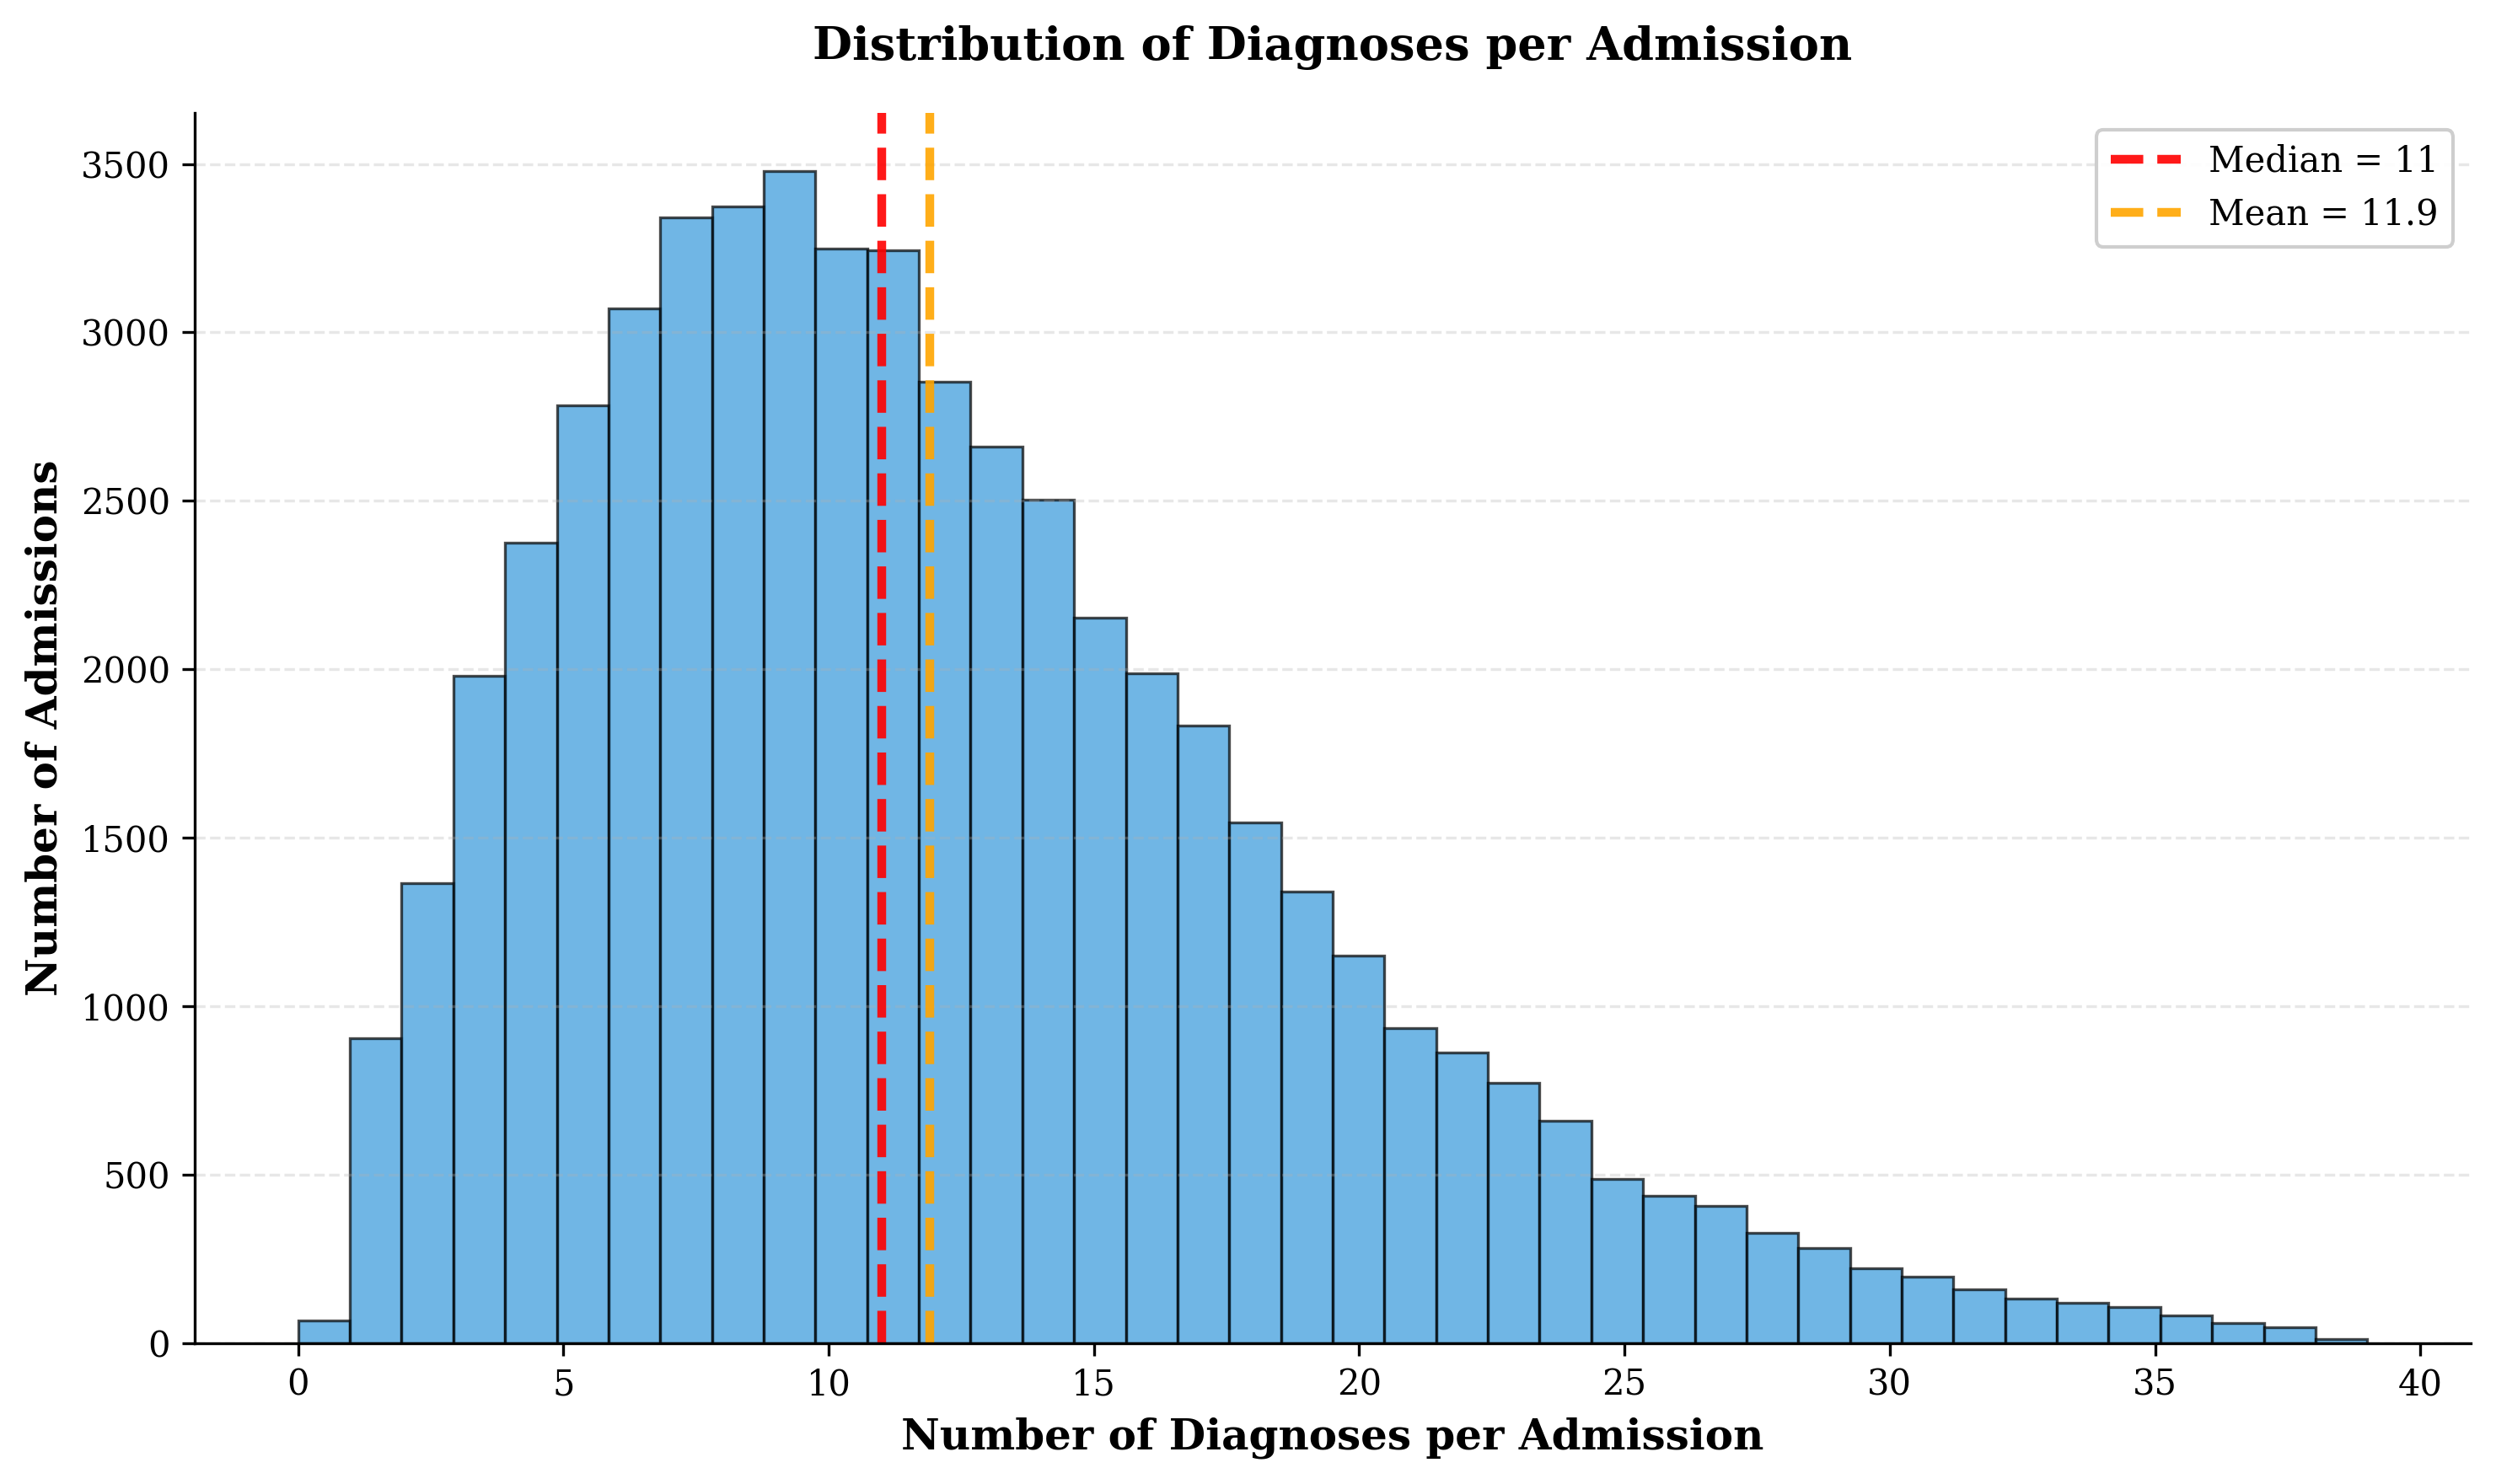
\includegraphics[width=0.8\textwidth]{Images/thesis_plots/diagnoses_per_admission_hist.png}
    \caption{Distribution of the number of diagnosis codes per admission. Dashed lines indicate median and mean.}
    \label{fig:diag-per-admission-hist}
\end{figure}

\begin{figure}[t]
    \centering
    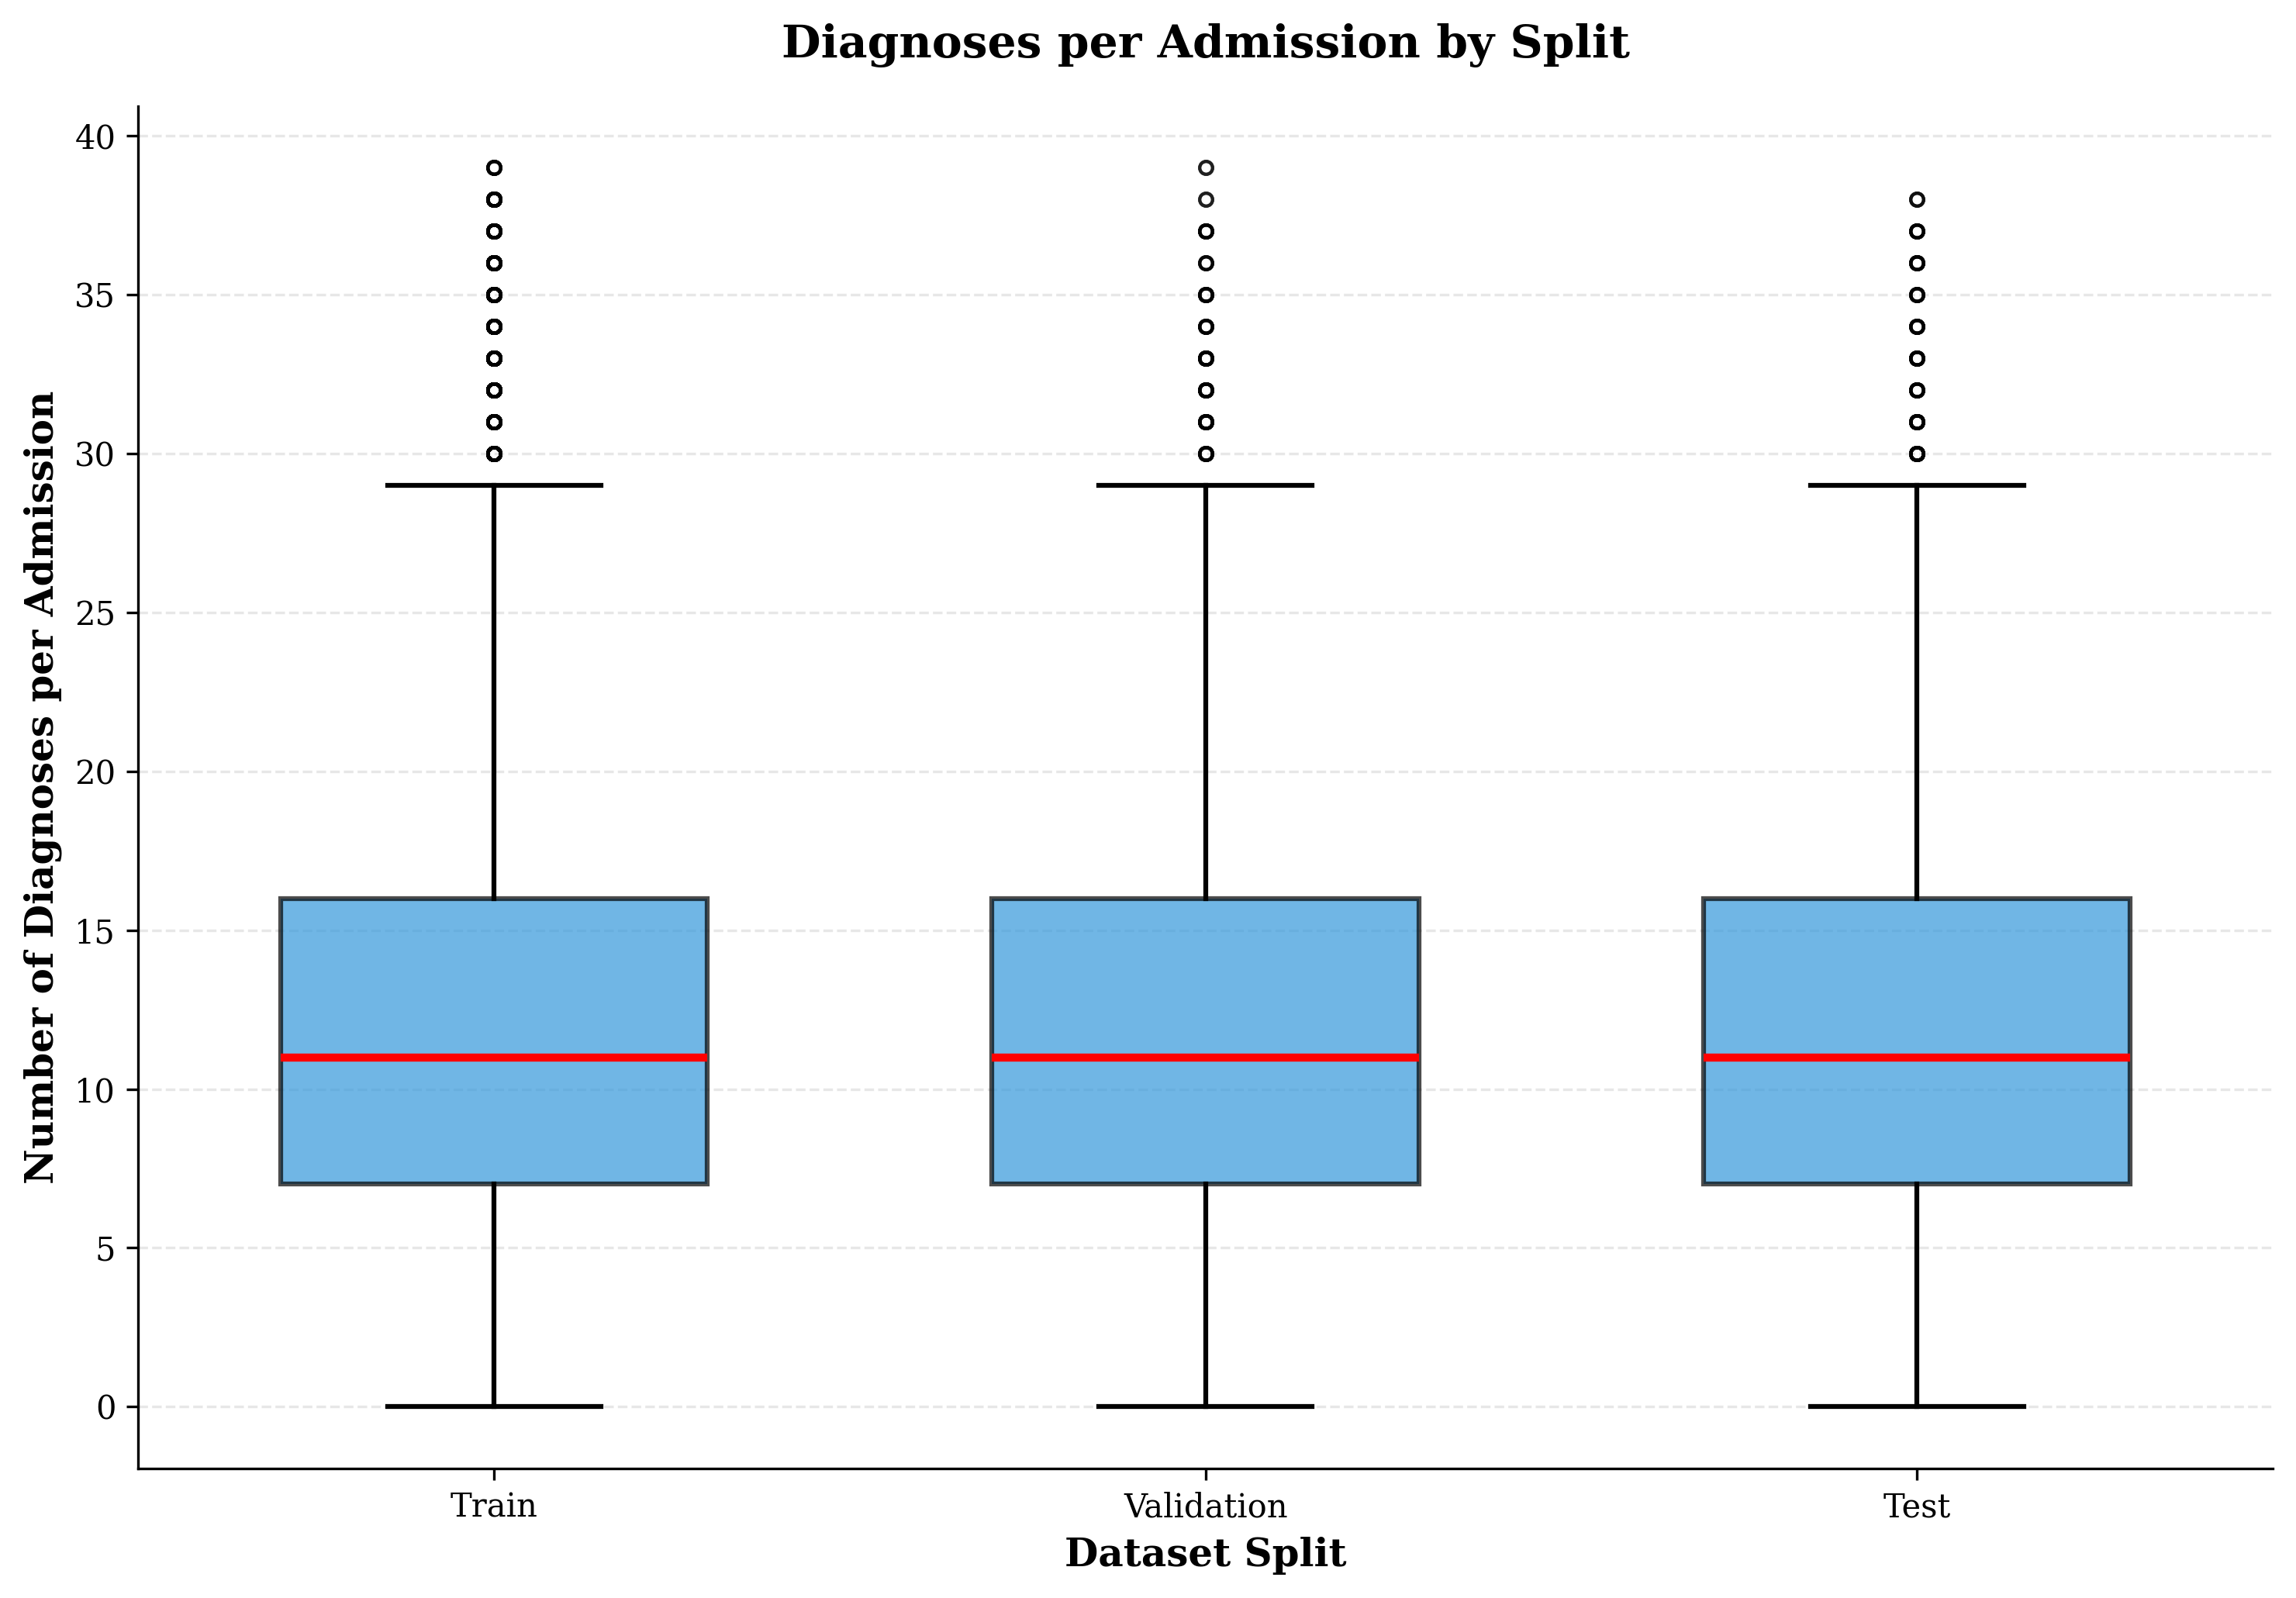
\includegraphics[width=0.7\textwidth]{Images/thesis_plots/diagnoses_per_admission_boxplot.png}
    \caption{Number of diagnoses per admission by dataset split. The three partitions exhibit similar distributions, indicating balanced multimorbidity across Train/Validation/Test.}
    \label{fig:diag-per-admission-box}
\end{figure}

Empirically, the median number of diagnoses per admission is close to $K=12$, motivating a fixed inference-time output budget of $K=12$ diagnoses for both TextGen and CodeGen. This budget is enforced via prompt instruction (``Maximum: $K$ lines'') and post-processing that selects at most $K$ unique predictions.
This does \emph{not} constrain supervision during fine-tuning: admissions may contain more than $K$ gold diagnoses and the model is trained on the full label signal.

For admissions with $L^{(i)} > K$, the maximum achievable recall is upper-bounded by
\begin{equation}
    R^{\max(i)}=\min\left(1,\frac{K}{L^{(i)}}\right),
\end{equation}
even for an oracle ranking, motivating budget-aware evaluation and the $K$-sensitivity analysis in Chapter~\ref{sec:results}.

% ============================================================
\subsection{Implications for Model Design and Evaluation}
\label{subsec:implications-cohort}

The cohort structure implies three modelling and evaluation requirements.

First, the heavy-tailed label space makes success on head codes insufficient; performance must be analysed on rare codes explicitly. We therefore report Head-50 and Tail-50($\cap$Test) metrics in Chapter~\ref{sec:results}.

Second, multimorbidity under a strict output budget means recall improvements must come from \emph{prioritisation} rather than unconstrained generation. This motivates knowledge augmentation as an inductive bias for ranking clinically related diagnoses under limited output slots.

Third, chapter- and parent-level aggregation motivates hierarchical evaluation at the parent (three-digit) level to capture clinically meaningful near misses (correct disease family but incorrect subtype).


% --------------------------------------------------------------------------------------------
\section{Knowledge Graph Construction}
\label{subsec:kg-construction}

A central component of this thesis is a clinical \emph{concept knowledge graph} (KG) that encodes biomedical background knowledge independently of any particular patient. The KG is \emph{ontology-centric}: nodes correspond to medical concepts (UMLS CUIs) rather than patient visits. It is used to support knowledge-augmented retrieval and path-based reasoning for both Task~1 and Task~2 (Section~\ref{sec:kg-integration}). In downstream usage, patient information is represented as a set of mapped concept nodes, and clinically relevant paths are retrieved from the KG to build a patient-conditioned medical index for diagnosis ranking.

\subsection{Design Principles}
\label{subsec:kg-design}

The KG is designed to satisfy three practical requirements:
\begin{enumerate}
    \item \textbf{Alignment with the cohort vocabularies.} KG entities must connect to the structured codes used in the processed MIMIC-IV cohort (diagnoses, procedures, medications, and laboratory tests).
    \item \textbf{Clinically meaningful semantics.} Edges should reflect interpretable biomedical relations (e.g., taxonomic links, anatomical sites, component structure, associations) rather than dataset-specific co-occurrence.
    \item \textbf{Tractable multi-hop connectivity.} The graph should enable short, informative paths between history concepts and candidate diagnoses while avoiding excessive fragmentation or overly dense expansions.
\end{enumerate}

\subsection{Ontology Sources and Concept Space}
\label{subsec:kg-sources}

The KG is constructed in the UMLS concept space~\cite{bodenreider2004umls}. Diagnoses and procedures from MIMIC-IV are mapped to UMLS CUIs via UMLS crosswalks, medications are represented at a pharmacologically meaningful abstraction level (ATC4 groups derived through NDC$\rightarrow$RxNorm$\rightarrow$ATC), and laboratory tests are linked to UMLS where mappings are available (via LOINC/UMLS when applicable). This yields a unified node space that supports cross-vocabulary reasoning (e.g., a medication concept connected to related diagnoses through pharmacologic or mechanism relations).

\subsection{Nodes and Relations}
\label{subsec:kg-nodes-relations}

\paragraph{Nodes.}
Each node is a UMLS Concept Unique Identifier (CUI). This representation naturally covers disease entities, procedures, findings, anatomical concepts, and a variety of biomedical intermediates that may bridge patient history to candidate diagnoses.

\paragraph{Relations.}
Each edge is labeled with \textbf{\texttt{rela}}, the relationship string (e.g., \texttt{isa}, \texttt{has\_finding\_site}, \texttt{has\_component}). In the final graph, the KG contains \textbf{348 distinct \texttt{rela}} relationship labels (Table~\ref{tab:kg-rela-top10}).

\subsubsection{Graph Statistics}
\label{subsubsec:kg-stats}

The final medical knowledge graph used in this thesis is a directed NetworkX graph. The graph contains \textbf{581,622 nodes} and \textbf{3,242,253 directed edges}, partitioned into \textbf{5,826 weakly connected components}. The largest connected component (LCC) dominates the structure with \textbf{572,462 nodes} and \textbf{3,233,301 edges}, indicating that most clinically relevant concepts are mutually reachable through short multi-hop paths.

Degree statistics show a moderately sparse but well-connected topology: the \textbf{average degree} is \textbf{11.15} (median \textbf{6}), with a \textbf{95th percentile degree} of \textbf{22}. A small number of highly connected hub nodes exist (maximum degree \textbf{60,063}), which is expected in UMLS-derived graphs due to broad taxonomy and highly generic biomedical concepts.

Edges are labeled using the relationship field \textbf{\texttt{rela}} (e.g., \texttt{isa}, \texttt{has\_finding\_site}, \texttt{has\_component}). Overall, the KG contains \textbf{348 distinct \texttt{rela}} relationship types, reflecting heterogeneous biomedical semantics while still allowing tractable short-path extraction under hop constraints (Section~\ref{sec:kg-integration}).


\begin{table}[t]
\centering
\caption{Summary statistics of the final medical knowledge graph used for retrieval and path linearization (\texttt{medical\_knowledge\_graph2.pkl}).}
\label{tab:kg-summary}
\begin{tabular}{l r}
\toprule
\textbf{Statistic} & \textbf{Value} \\
\midrule
Number of nodes $|\mathcal{V}|$ & 581{,}622 \\
Number of edges $|\mathcal{E}|$ & 3{,}242{,}253 \\
Connected components & 5{,}826 \\
Largest component: nodes & 572{,}462 \\
Largest component: edges & 3{,}233{,}301 \\
Isolated nodes & 0 \\
Average degree & 11.15 \\
Median degree & 6 \\
95th percentile degree & 22 \\
Maximum degree & 60{,}063 \\
\bottomrule
\end{tabular}
\end{table}


\begin{table}[t]
\centering
\caption{Most frequent relationship labels (\texttt{rela}) in the KG (top-10). These are dominated by taxonomic links and part--whole / site relations, which are particularly useful for short-path reasoning and clinically tolerant generalisation.}
\label{tab:kg-rela-top10}
\begin{tabular}{l r}
\toprule
\textbf{\texttt{relation}} & \textbf{Edge count} \\
\midrule
isa & 790{,}303 \\
inverse\_isa & 770{,}846 \\
component\_of & 250{,}482 \\
has\_component & 250{,}089 \\
has\_finding\_site & 198{,}718 \\
finding\_site\_of & 197{,}843 \\
class\_of & 195{,}543 \\
has\_class & 184{,}609 \\
\bottomrule
\end{tabular}
\end{table}


\subsection{Mapping Cohort Concepts to KG Nodes}
\label{subsec:kg-mapping}

To align patient data with the ontology-centric KG, each structured concept retained in the processed cohort is linked to one or more KG nodes (UMLS CUIs). This mapping provides a shared semantic identifier space across heterogeneous vocabularies (diagnoses, procedures, medications, and laboratory concepts) and enables two downstream capabilities: (i) graph-based relational evidence extraction between patient context and candidate diagnoses, and (ii) access to canonical concept names/descriptions for prompt construction (Section~\ref{subsubsec:textgen-prompt}).

Concretely, diagnosis and procedure codes are mapped through UMLS crosswalks into disease and intervention CUIs. Medications are first normalised by mapping MIMIC-IV NDC identifiers to RxNorm and aggregating to ATC4 groups; where UMLS links exist, these medication groups are connected to pharmacologic CUIs, enabling medication$\rightarrow$disease connectivity in the KG. For laboratory measurements, tests are linked to UMLS laboratory/measurement CUIs when mappings are available; discretised lab states (bins) are treated as feature-level symbols and are associated with their underlying base lab concept when KG reasoning uses laboratory information.

\paragraph{Patient-conditioned retrieval (subgraph induction).}
Rather than operating over the full KG during inference, the system conditions retrieval on the patient context by selecting the subset of KG nodes corresponding to: (i) the patient history concepts (from structured codes) and (ii) the candidate diagnosis concepts. Paths are then enumerated within this patient-relevant region (optionally including intermediate bridging concepts encountered along short multi-hop connections), and the resulting relational evidence is linearized to populate a patient-specific medical index used by the knowledge-augmented retrieval and reranking modules described in Section~\ref{sec:kg-integration}.
% --------------------------------------------------------------------------------------------
\section{Model Architectures}
\label{sec:model-architectures}

This section describes the modelling pipelines used for Task~1 (current-visit diagnosis prediction) and Task~2 (history-aware next-visit diagnosis prediction) as defined in Section~\ref{sec:problem-formulation}. In both tasks, prediction is formulated as \emph{conditional sequence generation} with an instruction-tuned, decoder-only Transformer language model. Models are implemented with Hugging Face \texttt{transformers}~\cite{wolf2020transformers} and adapted using parameter-efficient fine-tuning via LoRA~\cite{hu2021lora} on LLaMA-style backbones~\cite{touvron2023llama}. The task-dependent change is the \emph{prompt content} (single-admission vs.\ history-aware inputs; Section~\ref{sec:preprocessing} and Figure~\ref{fig:task2-history-decomposition}), while the core pipelines remain unchanged.

We study two complementary pipelines (Figure~\ref{fig:arch-pipeline}):

\begin{enumerate}
    \item \textbf{CodeGen (codes $\rightarrow$ codes).} A direct baseline that conditions on serialised structured codes and selected note sections, and generates ICD-9-CM diagnosis codes as the output sequence.
    \item \textbf{TextGen (descriptions $\rightarrow$ terms $\rightarrow$ codes).} A two-stage pipeline that first generates \emph{diagnosis terms} (natural-language phrases) and then maps them to ICD-9 codes using an external semantic retrieval layer (ICD Mapper).
\end{enumerate}

\begin{figure}[t]
    \centering
    \begin{subfigure}{0.49\textwidth}
        \centering
        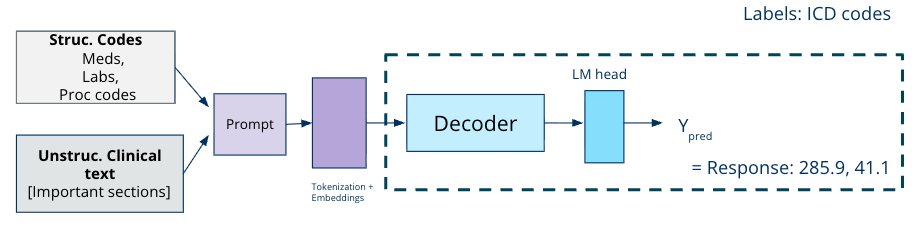
\includegraphics[width=\linewidth]{Images/CodeGen.png}
        \caption{CodeGen pipeline (direct ICD code generation).}
        \label{fig:codegen}
    \end{subfigure}\hfill
    \begin{subfigure}{0.49\textwidth}
        \centering
        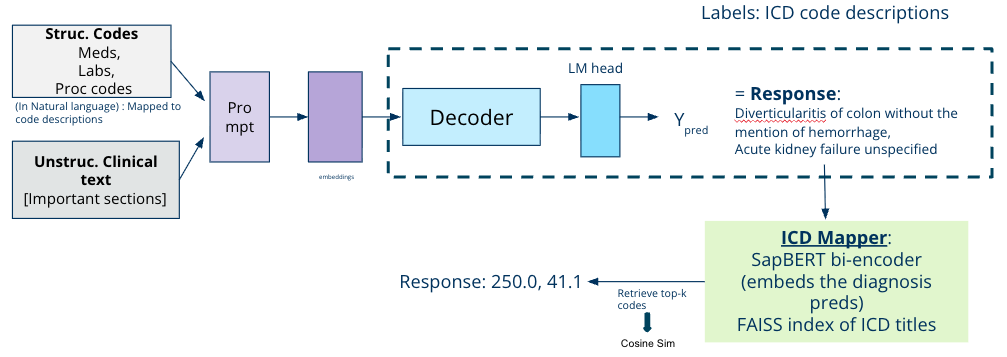
\includegraphics[width=\linewidth]{Images/TextGen.png}
        \caption{TextGen pipeline (term generation + ICD mapping).}
        \label{fig:textgen}
    \end{subfigure}
    \caption{Architecture overview of the two diagnosis prediction pipelines. Both consume the same multimodal admission representation but differ in the output space and post-processing.}
    \label{fig:arch-pipeline}
\end{figure}

\subsection{Backbone LLM and Parameter-Efficient Fine-Tuning}
\label{subsec:backbone-peft}

All experiments are conducted with decoder-only Transformer backbones drawn from the \textbf{LLaMA} and \textbf{Meditron} families. Concretely, three variants are used for both CodeGen and TextGen: \textbf{Llama-3.2-1B-Instruct} (general-purpose, small-footprint model), \textbf{Llama-3.1-8B-Instruct} (higher-capacity general-purpose model), and \textbf{Meditron-8B} (a LLaMA-style model further trained on biomedical and clinical corpora, targeted at medical reasoning)~\cite{touvron2023llama,chen2023meditron}. The 1B model serves as an efficiency baseline that can be realistically deployed in resource-constrained settings, whereas the 8B models probe the impact of increased capacity and domain-oriented pre-training on diagnosis prediction. Unless otherwise stated, architectural and optimisation settings are kept identical across backbones so that performance differences can be attributed primarily to model capacity and pre-training domain.

All three backbones share the same core architecture: a causal (left-to-right) decoder-only Transformer with multi-head self-attention and position-wise feed-forward layers~\cite{vaswani2017attention,touvron2023llama}. Tokenisation uses a subword byte-pair encoding (BPE) scheme~\cite{sennrich2016neural}. For batching, the end-of-sequence token is re-used as the padding token. During fine-tuning, key-value (KV) caching is disabled to support gradient checkpointing and reduce GPU memory pressure.

To make fine-tuning feasible on long clinical prompts, all backbones are adapted using \textbf{Low-Rank Adaptation (LoRA)}~\cite{hu2021lora}. Rather than updating all Transformer weights, low-rank adaptation matrices are attached to selected attention and feed-forward projections, and only these adapter parameters are updated while the base model remains frozen. Unless stated otherwise, we use:
\begin{itemize}
    \item a moderate LoRA rank (e.g.\ $r=16$) with scaling (e.g.\ $\alpha=32$),
    \item a small LoRA dropout (e.g.\ 0.05),
    \item updates restricted to LoRA parameters (and, where applicable, a small set of auxiliary parameters such as selected normalisation terms).
\end{itemize}

Optimisation settings and early stopping are described in Section~\ref{sec:training}.

\subsection{CodeGen: Direct ICD-9 Code Generation}
\label{subsec:codegen-arch}

CodeGen treats diagnosis prediction as direct generation in the ICD-9 code space. The model receives a linearised multimodal prompt containing:
(i) a compact visit header,
(ii) a structured summary (demographics + pruned code lists from Section~\ref{sec:preprocessing}),
(iii) selected clinical note sections, and
(iv) an instruction that constrains the output format to \emph{ICD codes only}.

\paragraph{Prompt structure (high level).}
\begin{itemize}
    \item \textbf{Header:} admission identifiers (\texttt{subject\_id}, \texttt{hadm\_id})
    \item \textbf{Structured block:} demographics and code lists (diagnoses/procedures/medications/labs as applicable)
    \item \textbf{Text block:} Task-specific discharge-summary sections (Section~\ref{sec:preprocessing})
    \item \textbf{Instruction + answer tag:} explicitly requests ICD-9-CM codes and nothing else
\end{itemize}

\paragraph{Illustrative prompt example (CodeGen).}
\begin{tcolorbox}[title={Example Codegen prompt for a single admission},colback=gray!3,colframe=black!30,breakable]
\small
\begin{verbatim}
[VISIT] subject_id=12345 hadm_id=67890
[DEM] gender=F age_group=60-69 stay_days=7 death=0
[NDC] 00093015005 00093015010 ...
[PROC] 39.61 88.56 ...
[LAB] 2345-7 718-7 2075-0 ...

[CHIEF COMPLAINT] Shortness of breath and leg swelling for 3 days.
[HISTORY OF PRESENT ILLNESS] 68-year-old female with history of CHF and DM2 ...
[PAST MEDICAL HISTORY] Congestive heart failure, type 2 diabetes mellitus ...
[PHYSICAL EXAM] Bibasilar crackles, elevated JVP, pitting edema ...
[PERTINENT RESULTS] BNP 1500, CXR: pulmonary edema ...
[BRIEF HOSPITAL COURSE] Treated with IV diuretics with improvement ...

[TASK] You are a medical coding expert. Based on the patient information above,
generate the appropriate ICD-9-CM diagnosis codes. Follow these guidelines:
1. List only the ICD-9 codes separated by spaces
2. Use proper ICD-9 format with decimal points (e.g., 428.0 not 4280)
3. Include only codes directly supported by the clinical information
4. Do not include any explanations or text besides the codes themselves
[CODES]
\end{verbatim}
\end{tcolorbox}

During fine-tuning, the gold ICD-9 codes are appended after \texttt{[CODES]} and the loss is applied only to the generated continuation. At inference, generated codes are parsed, de-duplicated, and truncated to the fixed output budget ($K=12$) used throughout the thesis (Section~\ref{subsec:complexity-cohort}).

\subsection{TextGen: Diagnosis-Term Generation with Semantic ICD Mapping}
\label{subsec:textgen-arch}

TextGen decomposes coding into (1) \textbf{diagnosis-term generation} and (2) \textbf{normalisation to ICD codes}. The model is prompted to output a short list of diagnosis phrases (one per line), which are then mapped to ICD-9 codes using a retrieval-based ICD Mapper.

\paragraph{Prompt structure (high level).}
TextGen uses the same underlying multimodal content, but presents structured concepts in a more \emph{language-friendly} form (e.g., concept titles/descriptions) and constrains the output to \emph{diagnosis terms} rather than codes:
\begin{itemize}
    \item \textbf{Visit + structured summary:} demographics and described concepts
    \item \textbf{Text block:} selected note sections (Task-dependent; leakage-controlled for Task~2)
    \item \textbf{Instruction:} ``one diagnosis per line'', ``no ICD codes'', and ``maximum $K$ lines''
\end{itemize}

\paragraph{Illustrative prompt example (TextGen).}
\begin{tcolorbox}[title={Example Textgen user prompt},colback=gray!3,colframe=black!30,breakable]
\small
\begin{verbatim}
[VISIT] subject_id=12345 hadm_id=67890
DEMOGRAPHICS: gender=F age_group=60-69
MEDICATIONS: A10A C09A ...
PROCEDURES: 39.61 88.56 ...
LAB TESTS: 2345-7 718-7 ...

Chief Complaint: Shortness of breath and leg swelling for 3 days.
History of Present Illness: 68-year-old female with known CHF and DM2 ...
Past Medical History: Congestive heart failure, type 2 diabetes mellitus ...
Physical Exam: Bibasilar crackles, elevated JVP, pitting edema ...
Brief Hospital Course: Treated with IV diuretics with improvement ...

[TASK] List the final clinical diagnoses for this admission.
[FORMAT]
- One diagnosis per line
- Avoid abbreviations if possible
- No ICD codes or explanations
- Maximum: 12 lines
[OUTPUT]
\end{verbatim}

\vspace{1mm}
\textit{Target assistant output (training):}
\begin{verbatim}
- Acute exacerbation of congestive heart failure
- Type 2 diabetes mellitus without complication
- Essential hypertension
\end{verbatim}
\end{tcolorbox}

The desired assistant response is a short list of diagnoses, for example:
\begin{verbatim}
- Acute exacerbation of congestive heart failure
- Type 2 diabetes mellitus without complication
- Essential hypertension
\end{verbatim}

For Task~2, the prompt is modified to include past historical diagnoses (diagnoses codes (descriptions) across all the visits), while the output format remains unchanged.

\paragraph{ICD Mapper (SapBERT + FAISS).}
At inference, TextGen’s generated phrases are mapped to ICD-9 codes via semantic retrieval:
\begin{itemize}
    \item \textbf{Index:} ICD-9 titles/descriptions are embedded with a SapBERT-style bi-encoder~\cite{liu2020self} and stored in a FAISS index for efficient nearest-neighbour search~\cite{johnson2019billion}.
    \item \textbf{Query:} each generated diagnosis phrase is embedded with the same encoder and used to retrieve top-$k$ ICD candidates by cosine similarity.
    \item \textbf{Selection:} candidates can be filtered by a similarity threshold and optionally re-ranked with lightweight lexical matching; the best remaining match is selected as the mapped ICD-9 code.
\end{itemize}
Mapped codes are aggregated and de-duplicated at the admission level and truncated to the same output budget $K=12$ for evaluation consistency.

\paragraph{Reuse across tasks.}
Both CodeGen and TextGen are applied to Task~1 and Task~2 by changing only the prompt content to reflect the cohort construction and leakage constraints in Section~\ref{sec:preprocessing}. The backbone, fine-tuning procedure, decoding, and the ICD Mapper remain unchanged across tasks.

% --------------------------------------------------------------------------------------------
% \section{Training Procedure and Implementation Details}
% \label{sec:training}

% This section summarises the optimisation setup, implementation details, and stability measures used for training the Codegen and Textgen models on the multimodal EHR datasets.

% \subsection{Implementation Framework}
% \label{subsec:framework}

% All models are implemented using the Hugging Face \texttt{transformers} library~\cite{wolf2020transformers} and trained with its high-level training loop, combined with a LoRA-based parameter-efficient fine-tuning library~\cite{hu2021lora}. The overall pipeline comprises:

% \begin{itemize}
%     \item construction of multimodal prompts and targets from preprocessed tabular data,
%     \item tokenisation with dynamic padding to the longest sequence in each batch,
%     \item mixed-precision training on GPUs,
%     \item periodic evaluation on a held-out validation set and model checkpointing based on validation loss.
% \end{itemize}

% For Codegen, training is performed in a single-GPU setting with distributed data parallelism explicitly disabled to avoid unnecessary complexity. For Textgen, the training loop is compatible with multi-GPU training (via PyTorch Distributed Data Parallel) and includes additional safeguards to ensure robust initialisation and shutdown of the distributed backend.

% In terms of model variants, all experiments are conducted with decoder-only Transformer backbones drawn from the LLaMA and Meditron families. Concretely, three variants are used for both pipelines: \texttt{Llama-3.2-1B-Instruct} (general-purpose, small footprint), \texttt{Llama-3.1-8B-Instruct} (higher-capacity general model), and \texttt{Meditron-8B} (a LLaMA-style model further pre-trained on large-scale biomedical and clinical corpora, intended for medical reasoning tasks). The 1B model serves as an efficiency baseline that can be realistically deployed in resource-constrained settings, whereas the 8B models allow us to probe the impact of increased capacity and domain-specific pre-training on neuro-symbolic diagnosis prediction. Unless otherwise stated, architectural and optimisation settings are kept identical across backbones so that differences in performance can be attributed primarily to model capacity and pre-training domain.

% For \textbf{Task~1} (current-visit diagnosis prediction), we therefore train and evaluate \emph{both} Codegen and Textgen pipelines with all three backbone models, yielding a full $2 \times 3$ grid of configurations under a common training setup. For \textbf{Task~2} (next-visit diagnosis prediction), we deliberately restrict experiments to the Textgen pipeline only, again with all three backbones. This design choice is informed by the Task~1 evaluation (see Section~\ref{sec:results-task1}), where Textgen consistently outperforms Codegen across metrics and model sizes, reflecting the advantage of first generating diagnosis terms in natural language before mapping them to ICD-9 codes. Since Task~2 depends even more strongly on understanding and extrapolating from narrative clinical text, we consider Textgen the more appropriate and empirically superior architecture and therefore do not re-train a clearly weaker Codegen baseline for this longitudinal setting.

% The corresponding training and validation loss curves for all model--pipeline combinations are shown in Figures~\ref{fig:task1-codegen-training}--\ref{fig:task2-textgen-training}. These plots summarise the optimisation behaviour (convergence speed, overfitting tendencies, and stability) for each configuration, while detailed predictive performance is reported in the Results chapter (Sections~\ref{sec:results-task1} and~\ref{sec:results-task2}).

% \begin{figure}[t]
%     \centering
%     \begin{subfigure}{0.32\textwidth}
%         \centering
%         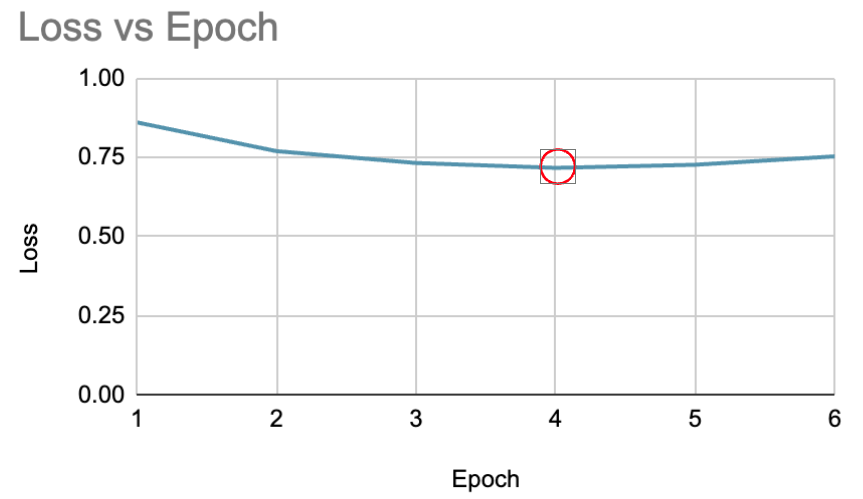
\includegraphics[width=\linewidth]{Images/train_temp.png}
%         \caption{Codegen -- Llama-3.2-1B}
%         \label{fig:task1-codegen-llama1b}
%     \end{subfigure}\hfill
%     \begin{subfigure}{0.32\textwidth}
%         \centering
%         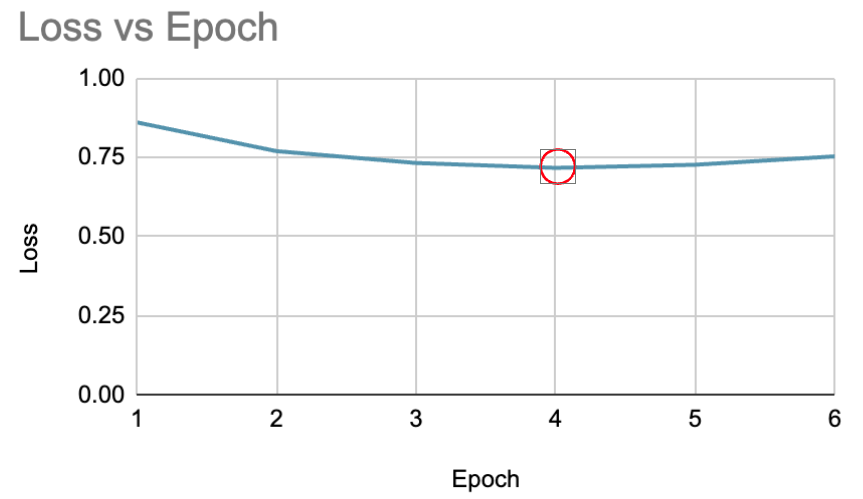
\includegraphics[width=\linewidth]{Images/train_temp.png}
%         \caption{Codegen -- Llama-3.1-8B}
%         \label{fig:task1-codegen-llama8b}
%     \end{subfigure}\hfill
%     \begin{subfigure}{0.32\textwidth}
%         \centering
%         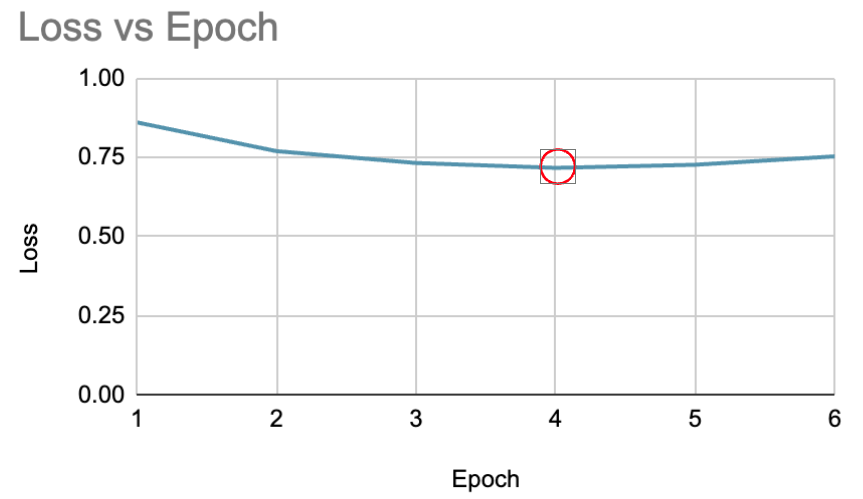
\includegraphics[width=\linewidth]{Images/train_temp.png}
%         \caption{Codegen -- Meditron-8B}
%         \label{fig:task1-codegen-meditron8b}
%     \end{subfigure}
%     \caption{Task~1 (current-visit diagnosis prediction), Codegen pipeline. Training and validation loss across epochs for each backbone model.}
%     \label{fig:task1-codegen-training}
% \end{figure}

% \begin{figure}[t]
%     \centering
%     \begin{subfigure}{0.5\textwidth}
%         \centering
%         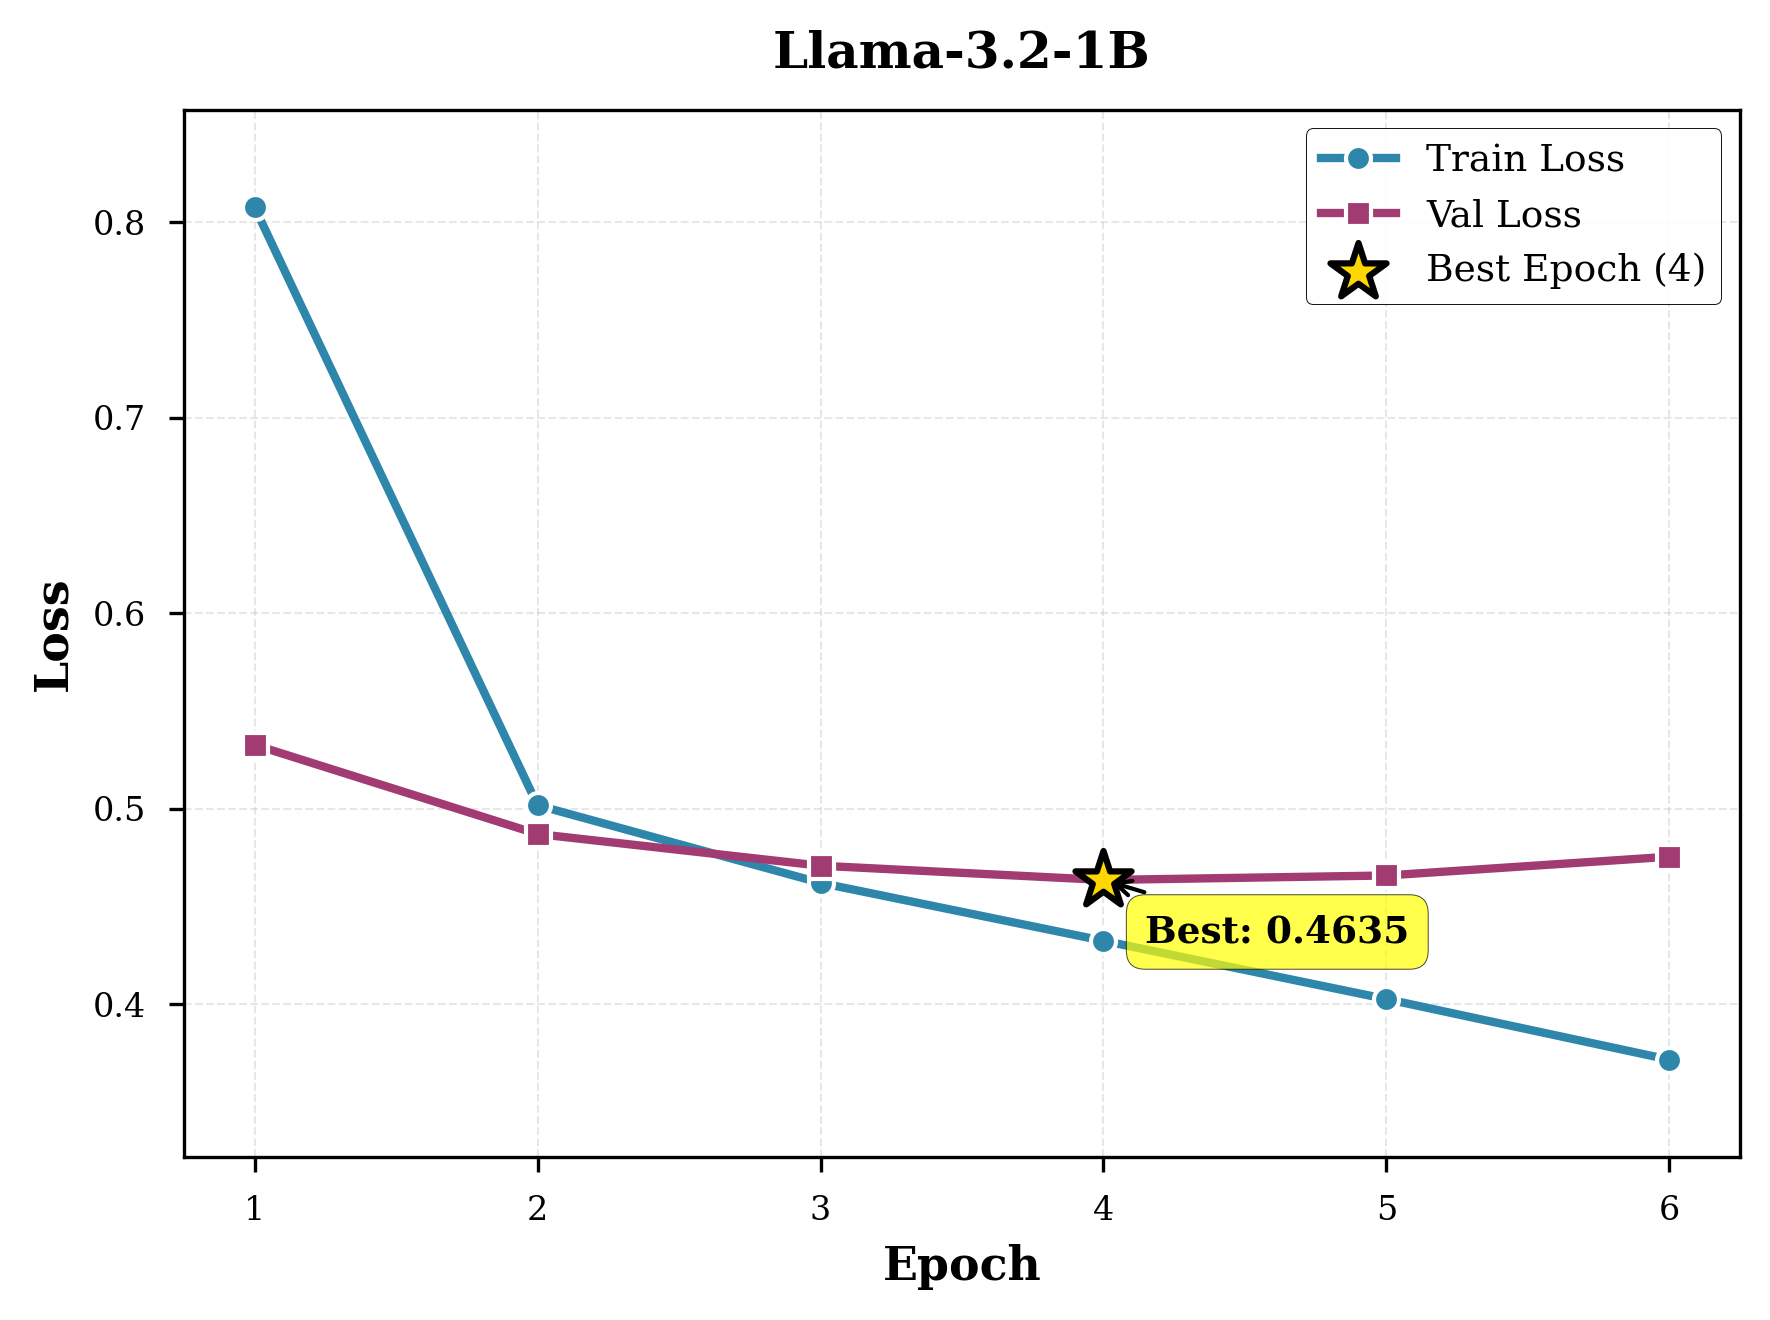
\includegraphics[width=\linewidth]{Images/training_curve_llama_32_1b.png}
%         \caption{Textgen -- Llama-3.2-1B}
%         \label{fig:task1-textgen-llama1b}
%     \end{subfigure}\hfill
%     \begin{subfigure}{0.5\textwidth}
%         \centering
%         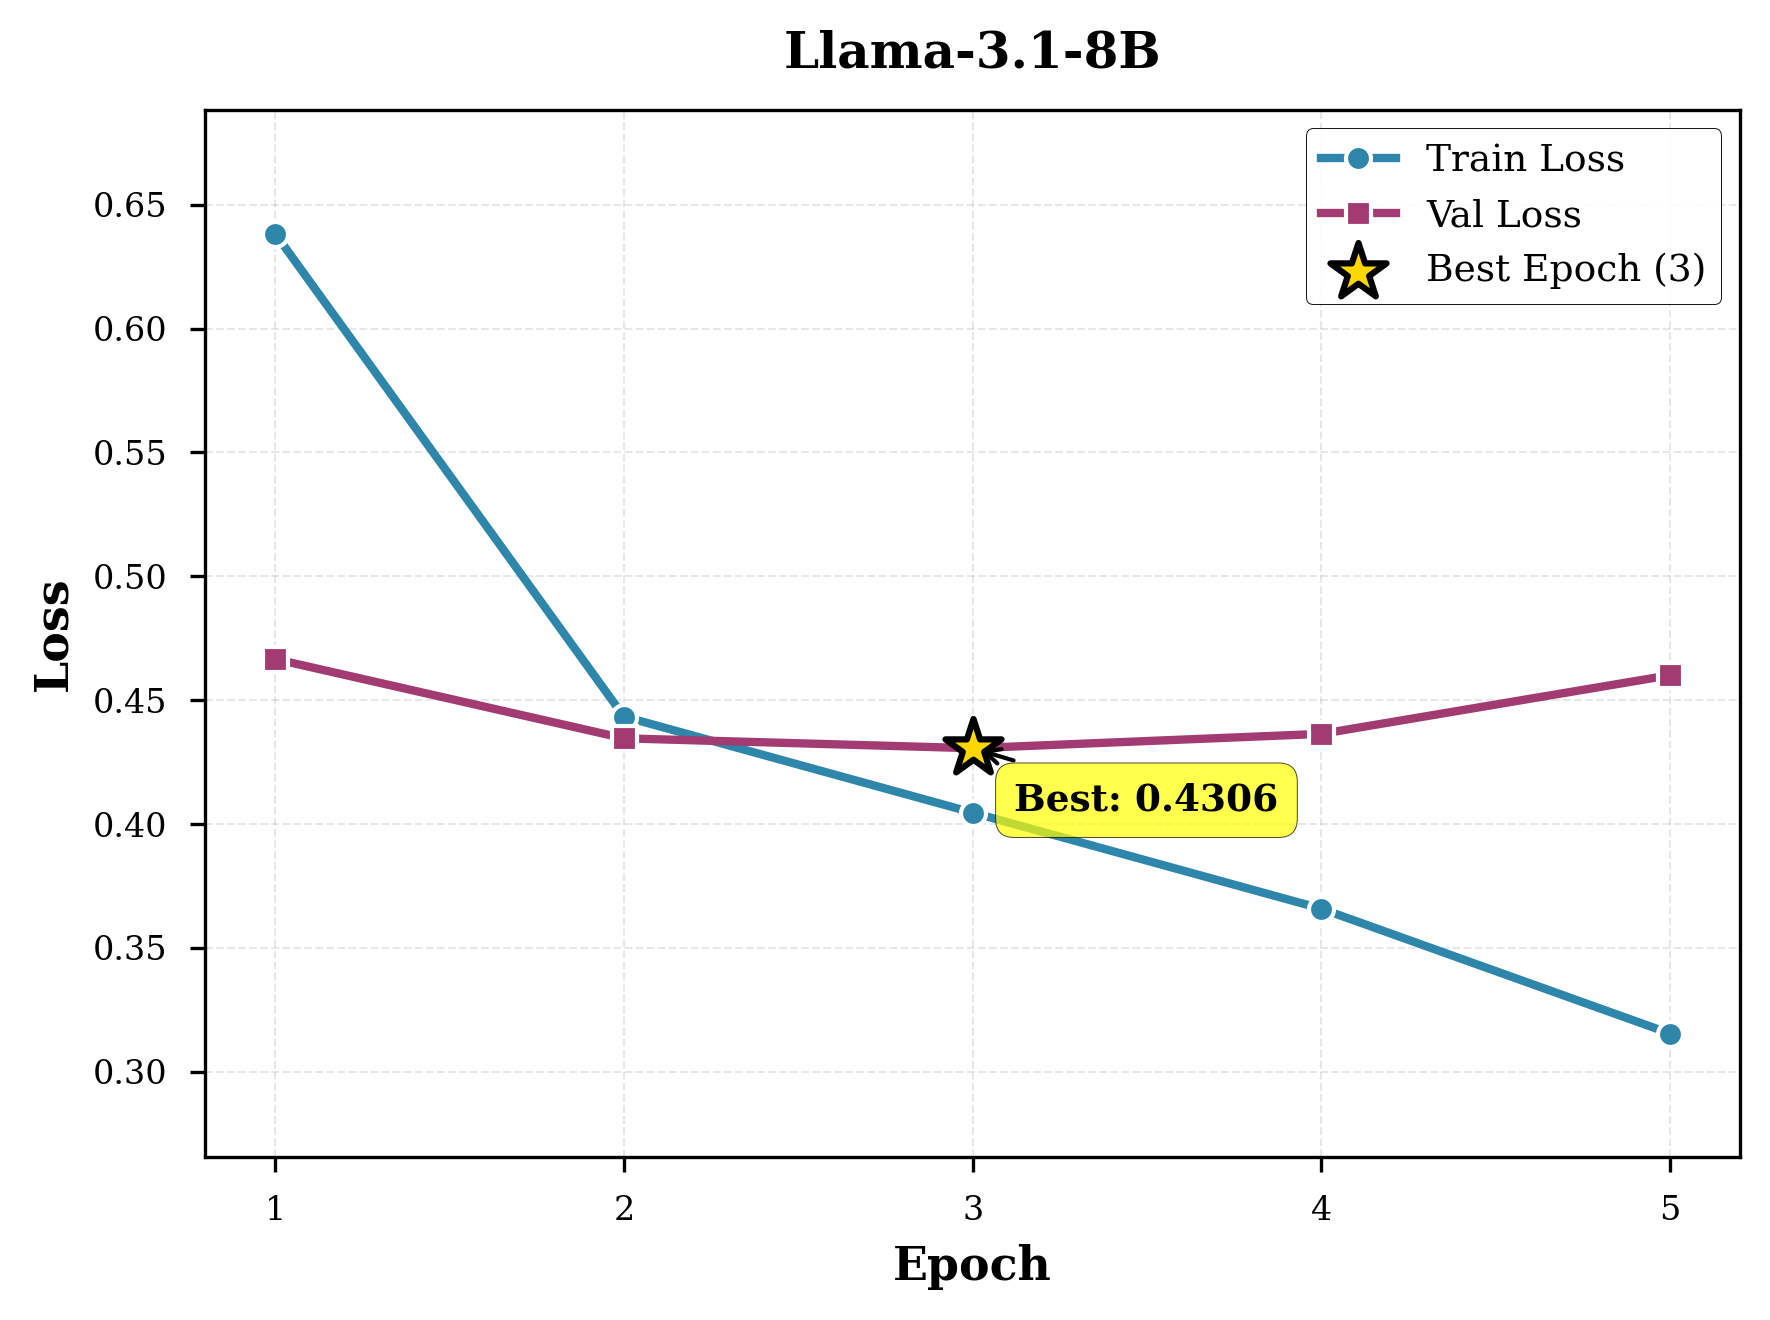
\includegraphics[width=\linewidth]{Images/training_curve_llama_31_8b.png}
%         \caption{Textgen -- Llama-3.1-8B}
%         \label{fig:task1-textgen-llama8b}
%     \end{subfigure}\hfill
%     \begin{subfigure}{0.5\textwidth}
%         \centering
%         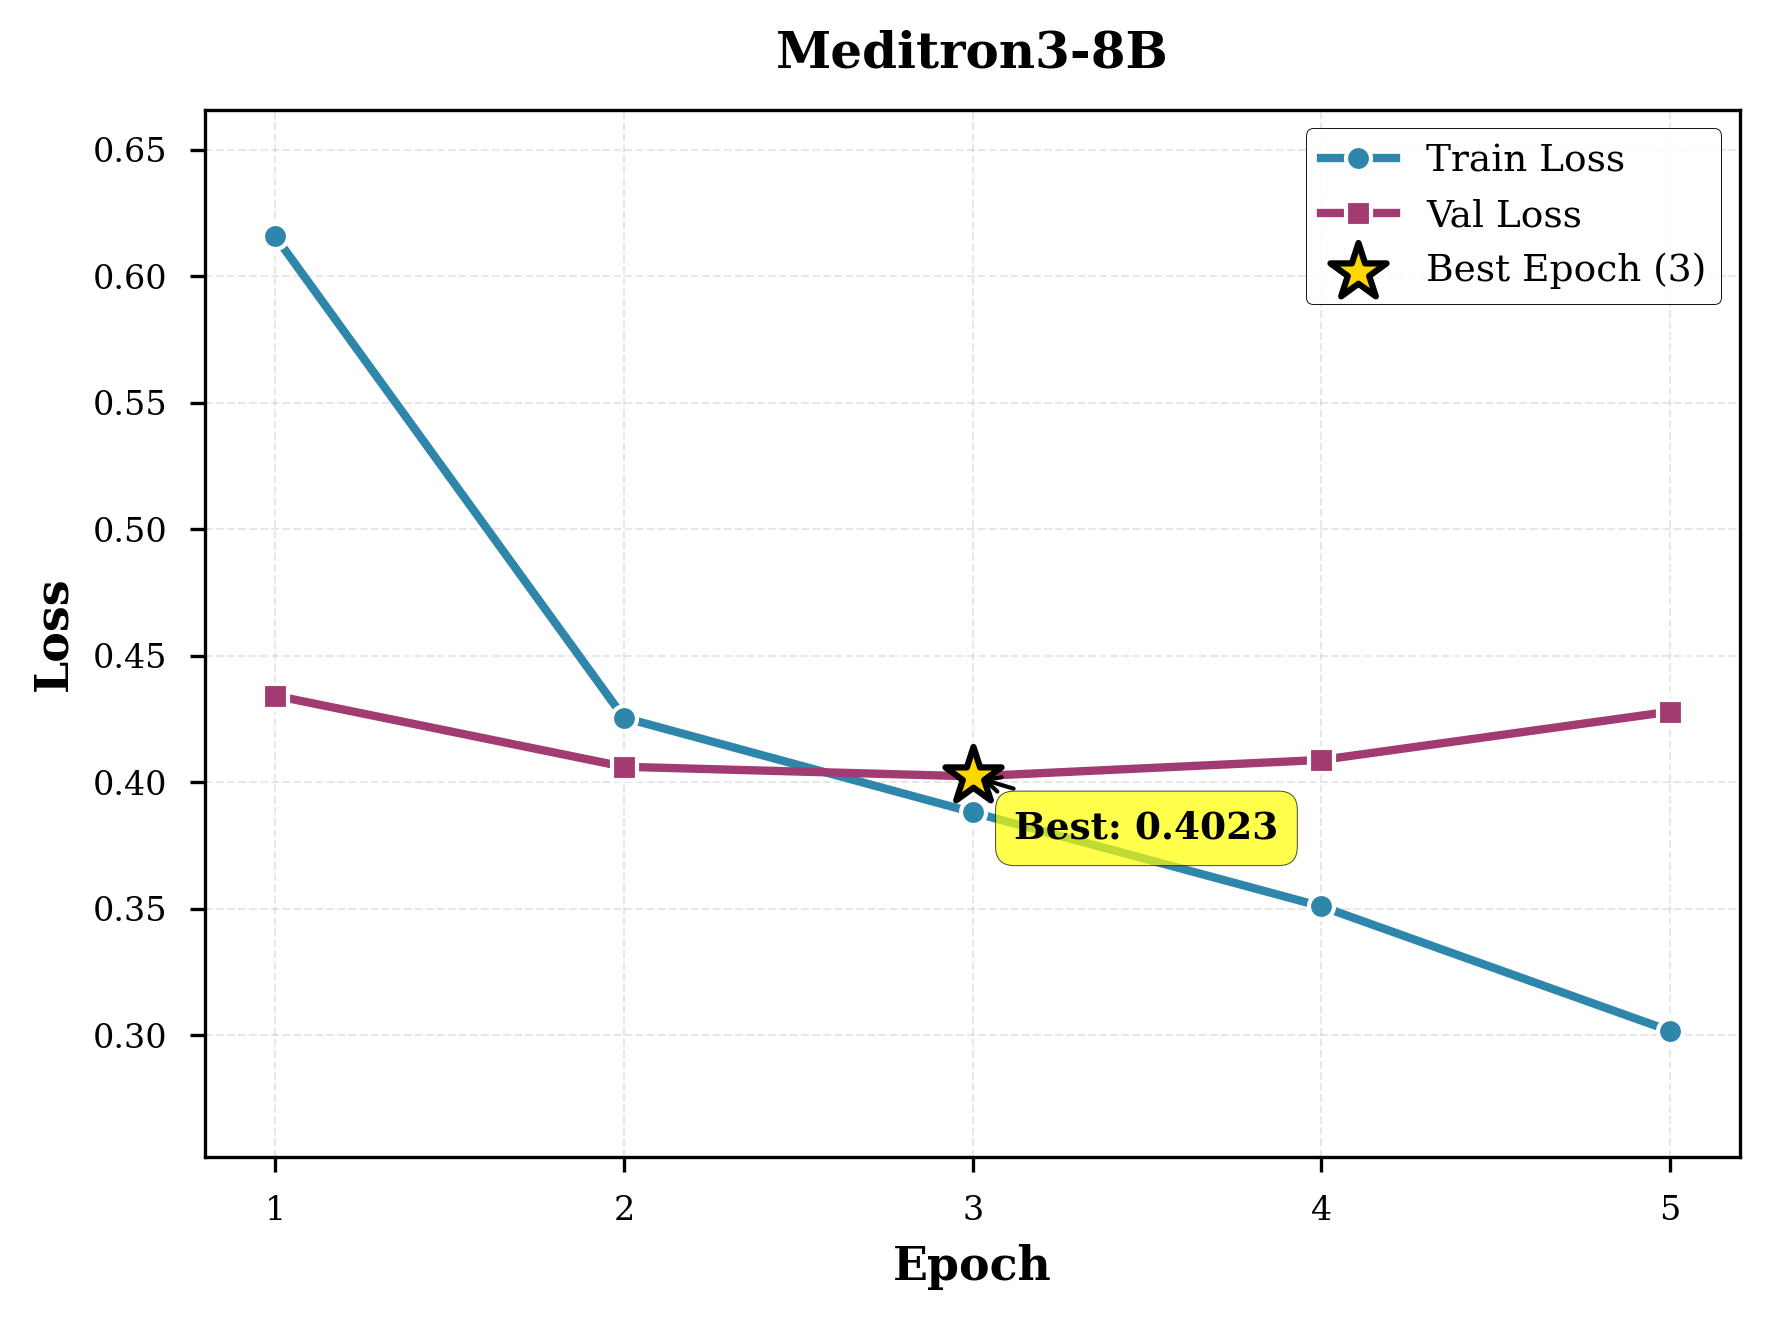
\includegraphics[width=\linewidth]{Images/training_curve_meditron3_8b.png}
%         \caption{Textgen -- Meditron-8B}
%         \label{fig:task1-textgen-meditron8b}
%     \end{subfigure}
%     \begin{subfigure}{0.5\textwidth}
%         \centering
%         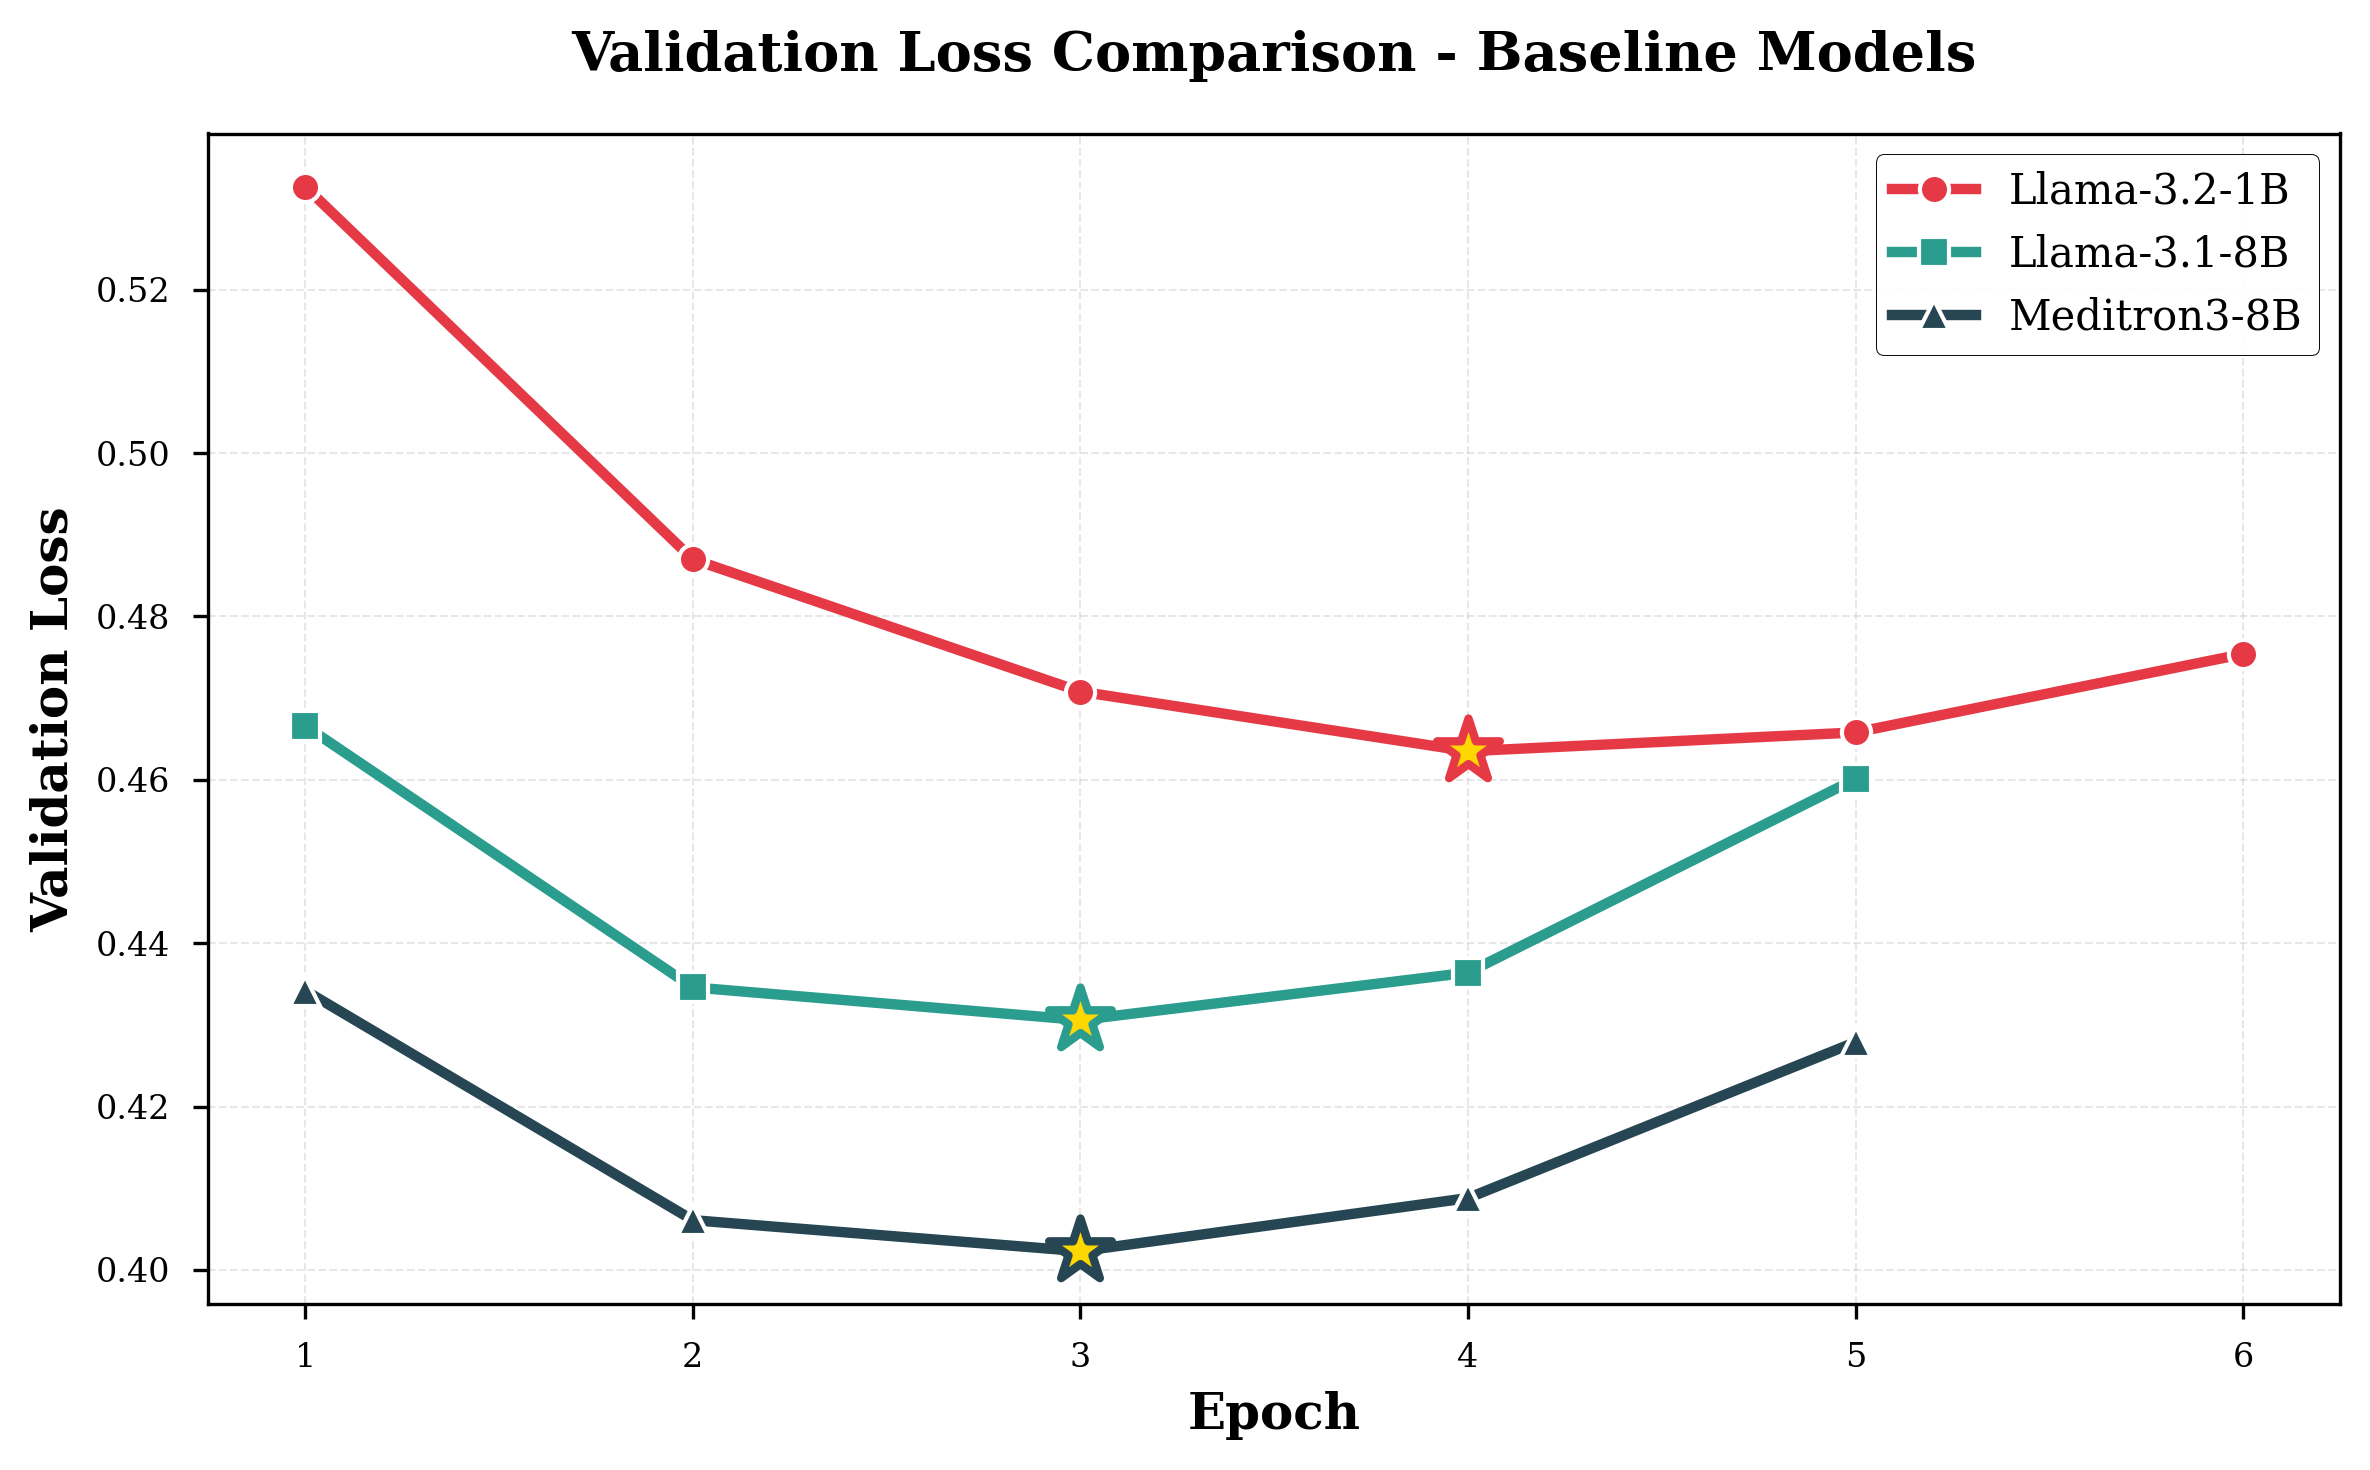
\includegraphics[width=\linewidth]{Images/validation_loss_comparison.png}
%         \caption{Val loss comparison}
%         \label{fig:task1-textgen-val-loss-comparison}
%     \end{subfigure}
%     \caption{Task~1 (current-visit diagnosis prediction), Textgen pipeline. Training and validation loss across epochs for each backbone model.}
%     \label{fig:task1-textgen-training}
% \end{figure}

% \begin{figure}[t]
%     \centering
%     \begin{subfigure}{0.5\textwidth}
%         \centering
%         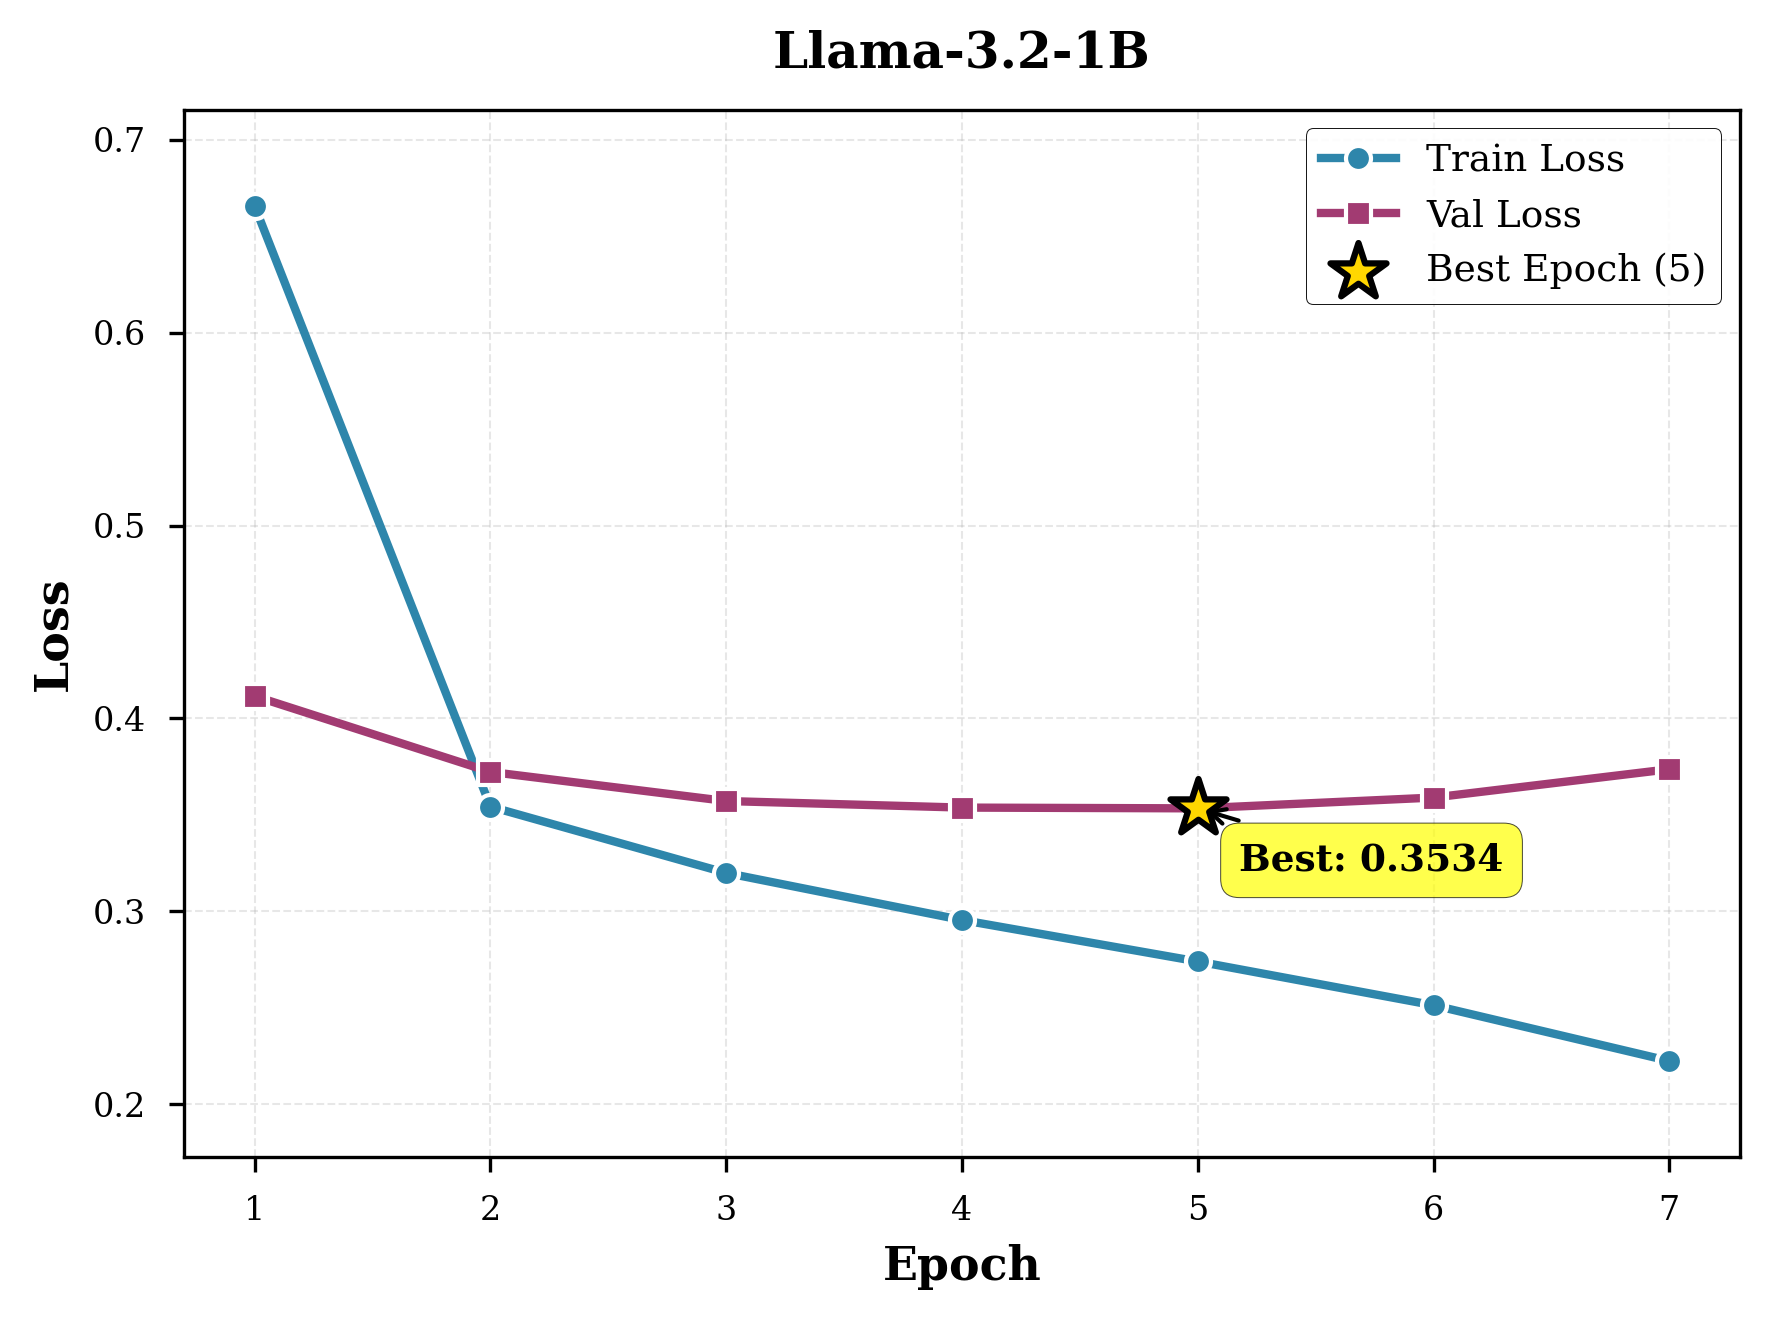
\includegraphics[width=\linewidth]{Images/training_curve_history_llama_32_1b.png}
%         \caption{Textgen -- Llama-3.2-1B}
%         \label{fig:task2-textgen-llama1b}
%     \end{subfigure}\hfill
%     \begin{subfigure}{0.5\textwidth}
%         \centering
%         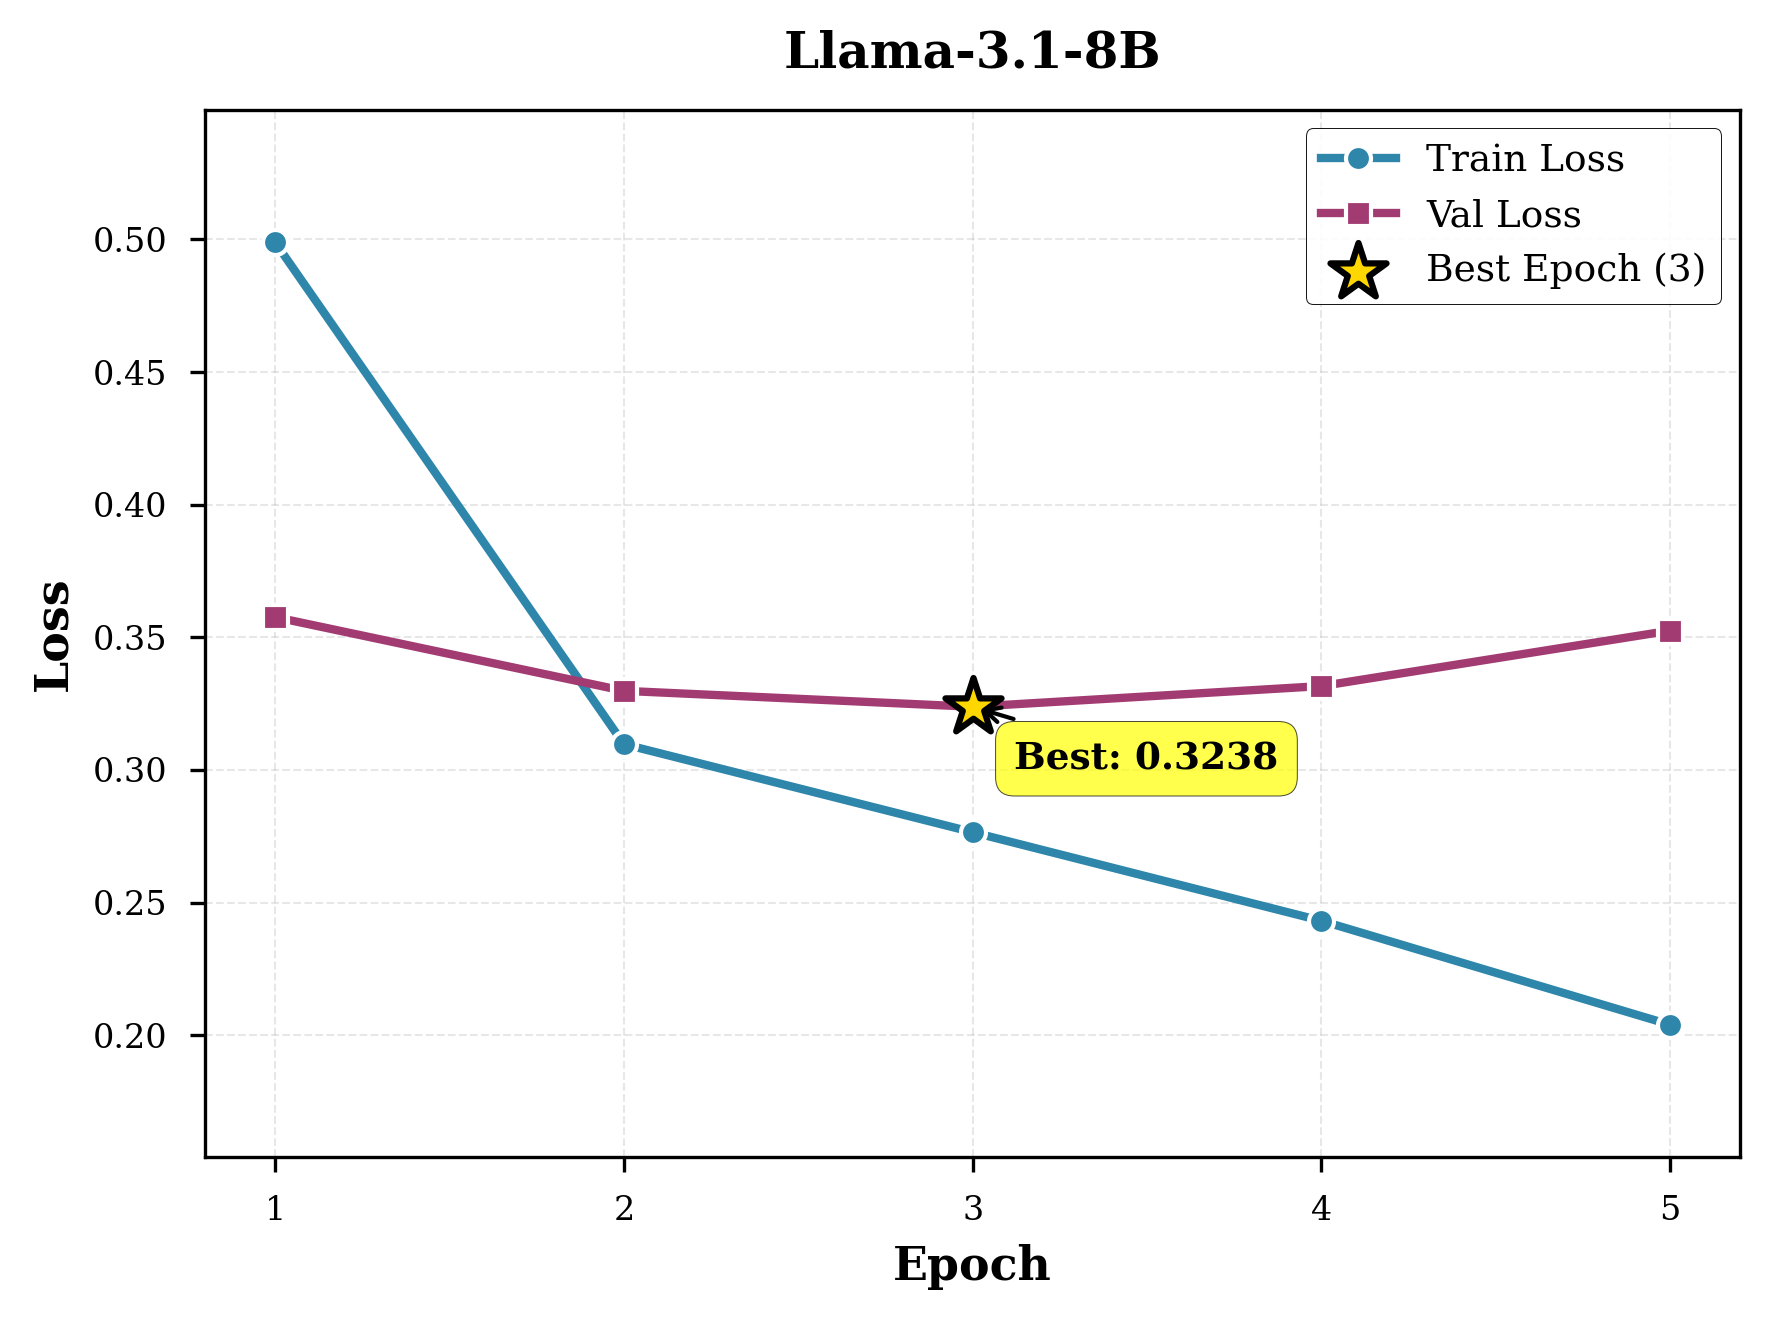
\includegraphics[width=\linewidth]{Images/training_curve_history_llama_31_8b.png}
%         \caption{Textgen -- Llama-3.1-8B}
%         \label{fig:task2-textgen-llama8b}
%     \end{subfigure}\hfill
%     \begin{subfigure}{0.5\textwidth}
%         \centering
%         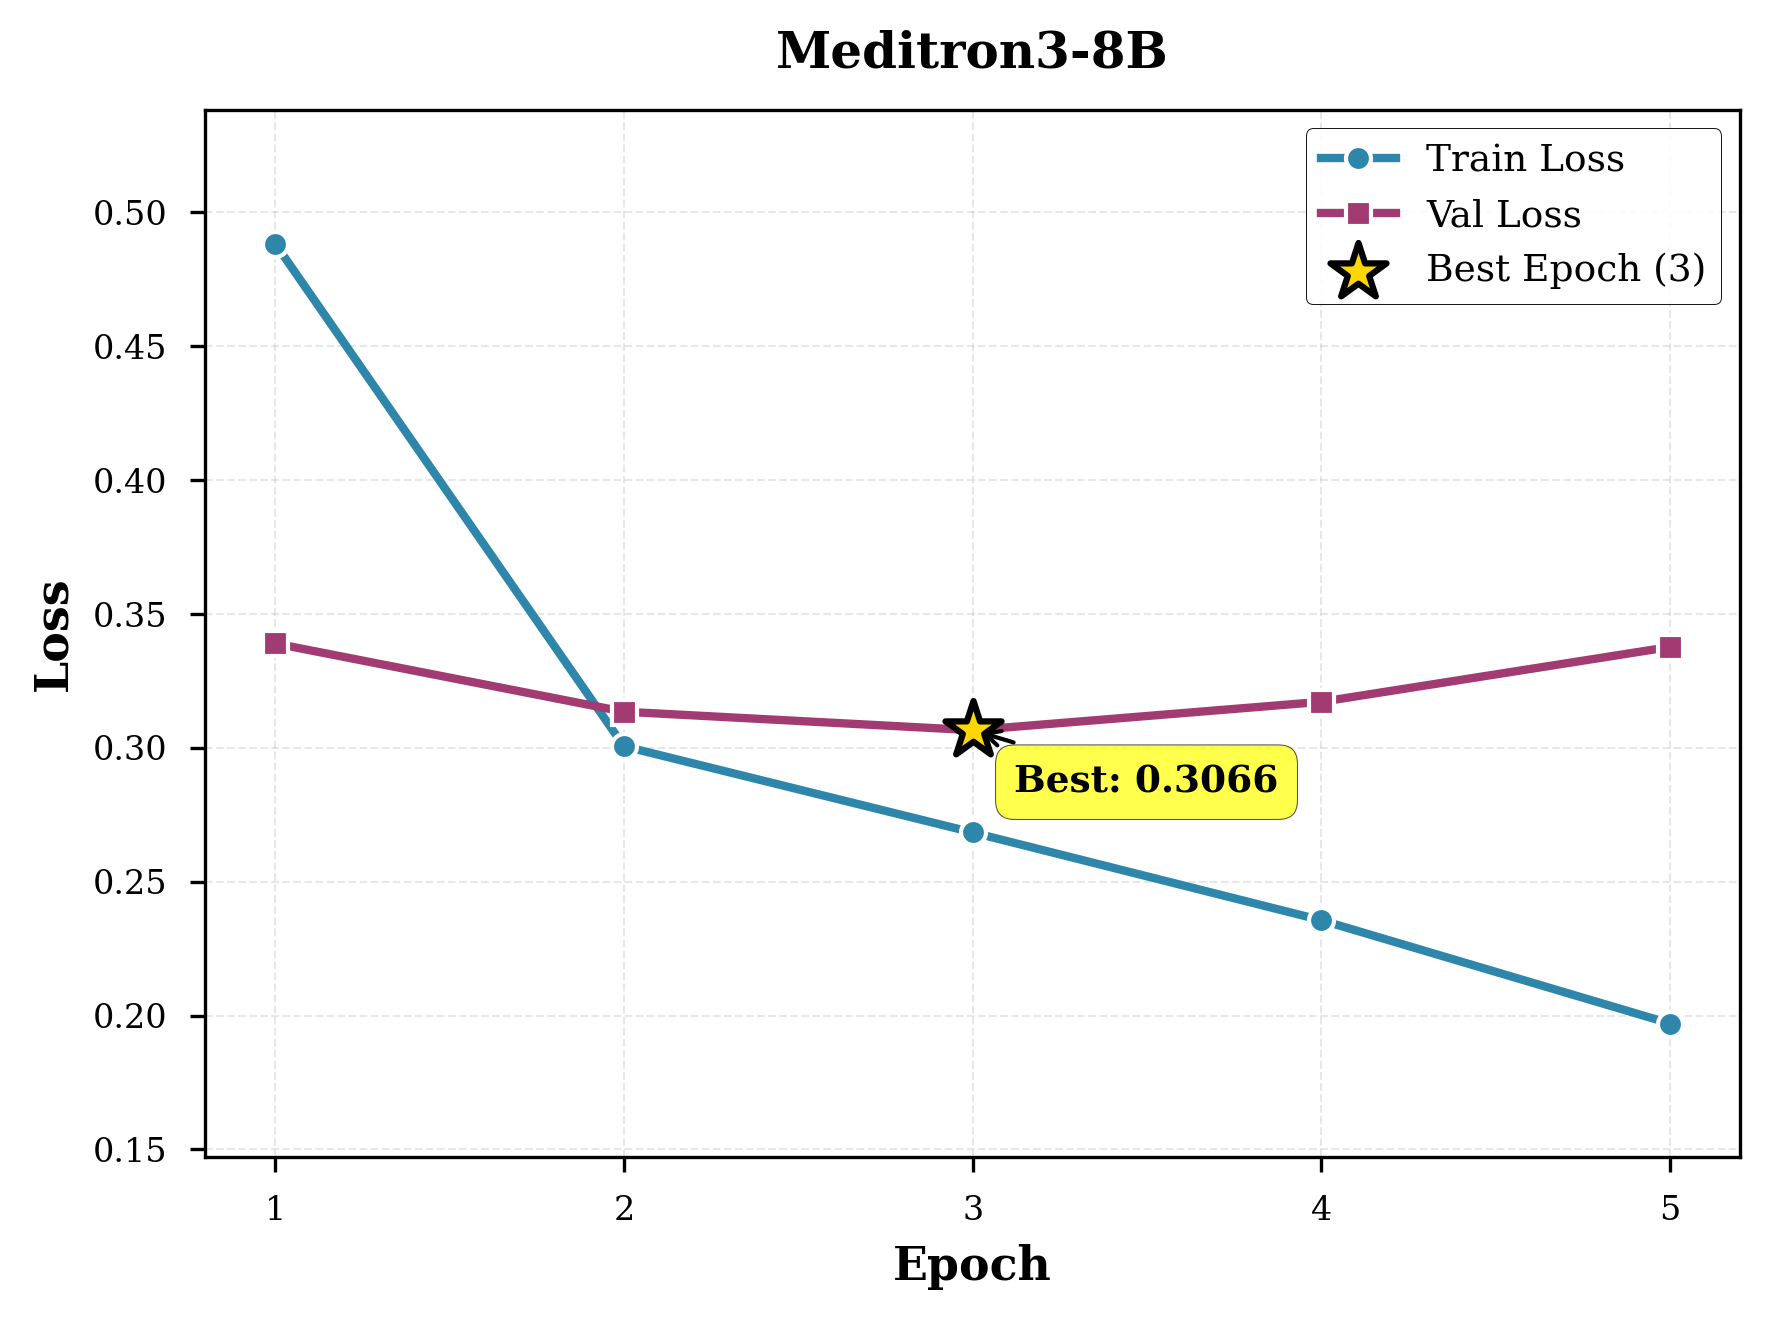
\includegraphics[width=\linewidth]{Images/training_curve_history_meditron3_8b.png}
%         \caption{Textgen -- Meditron-8B}
%         \label{fig:task2-textgen-meditron8b}
%     \end{subfigure}
%     \begin{subfigure}{0.5\textwidth}
%         \centering
%         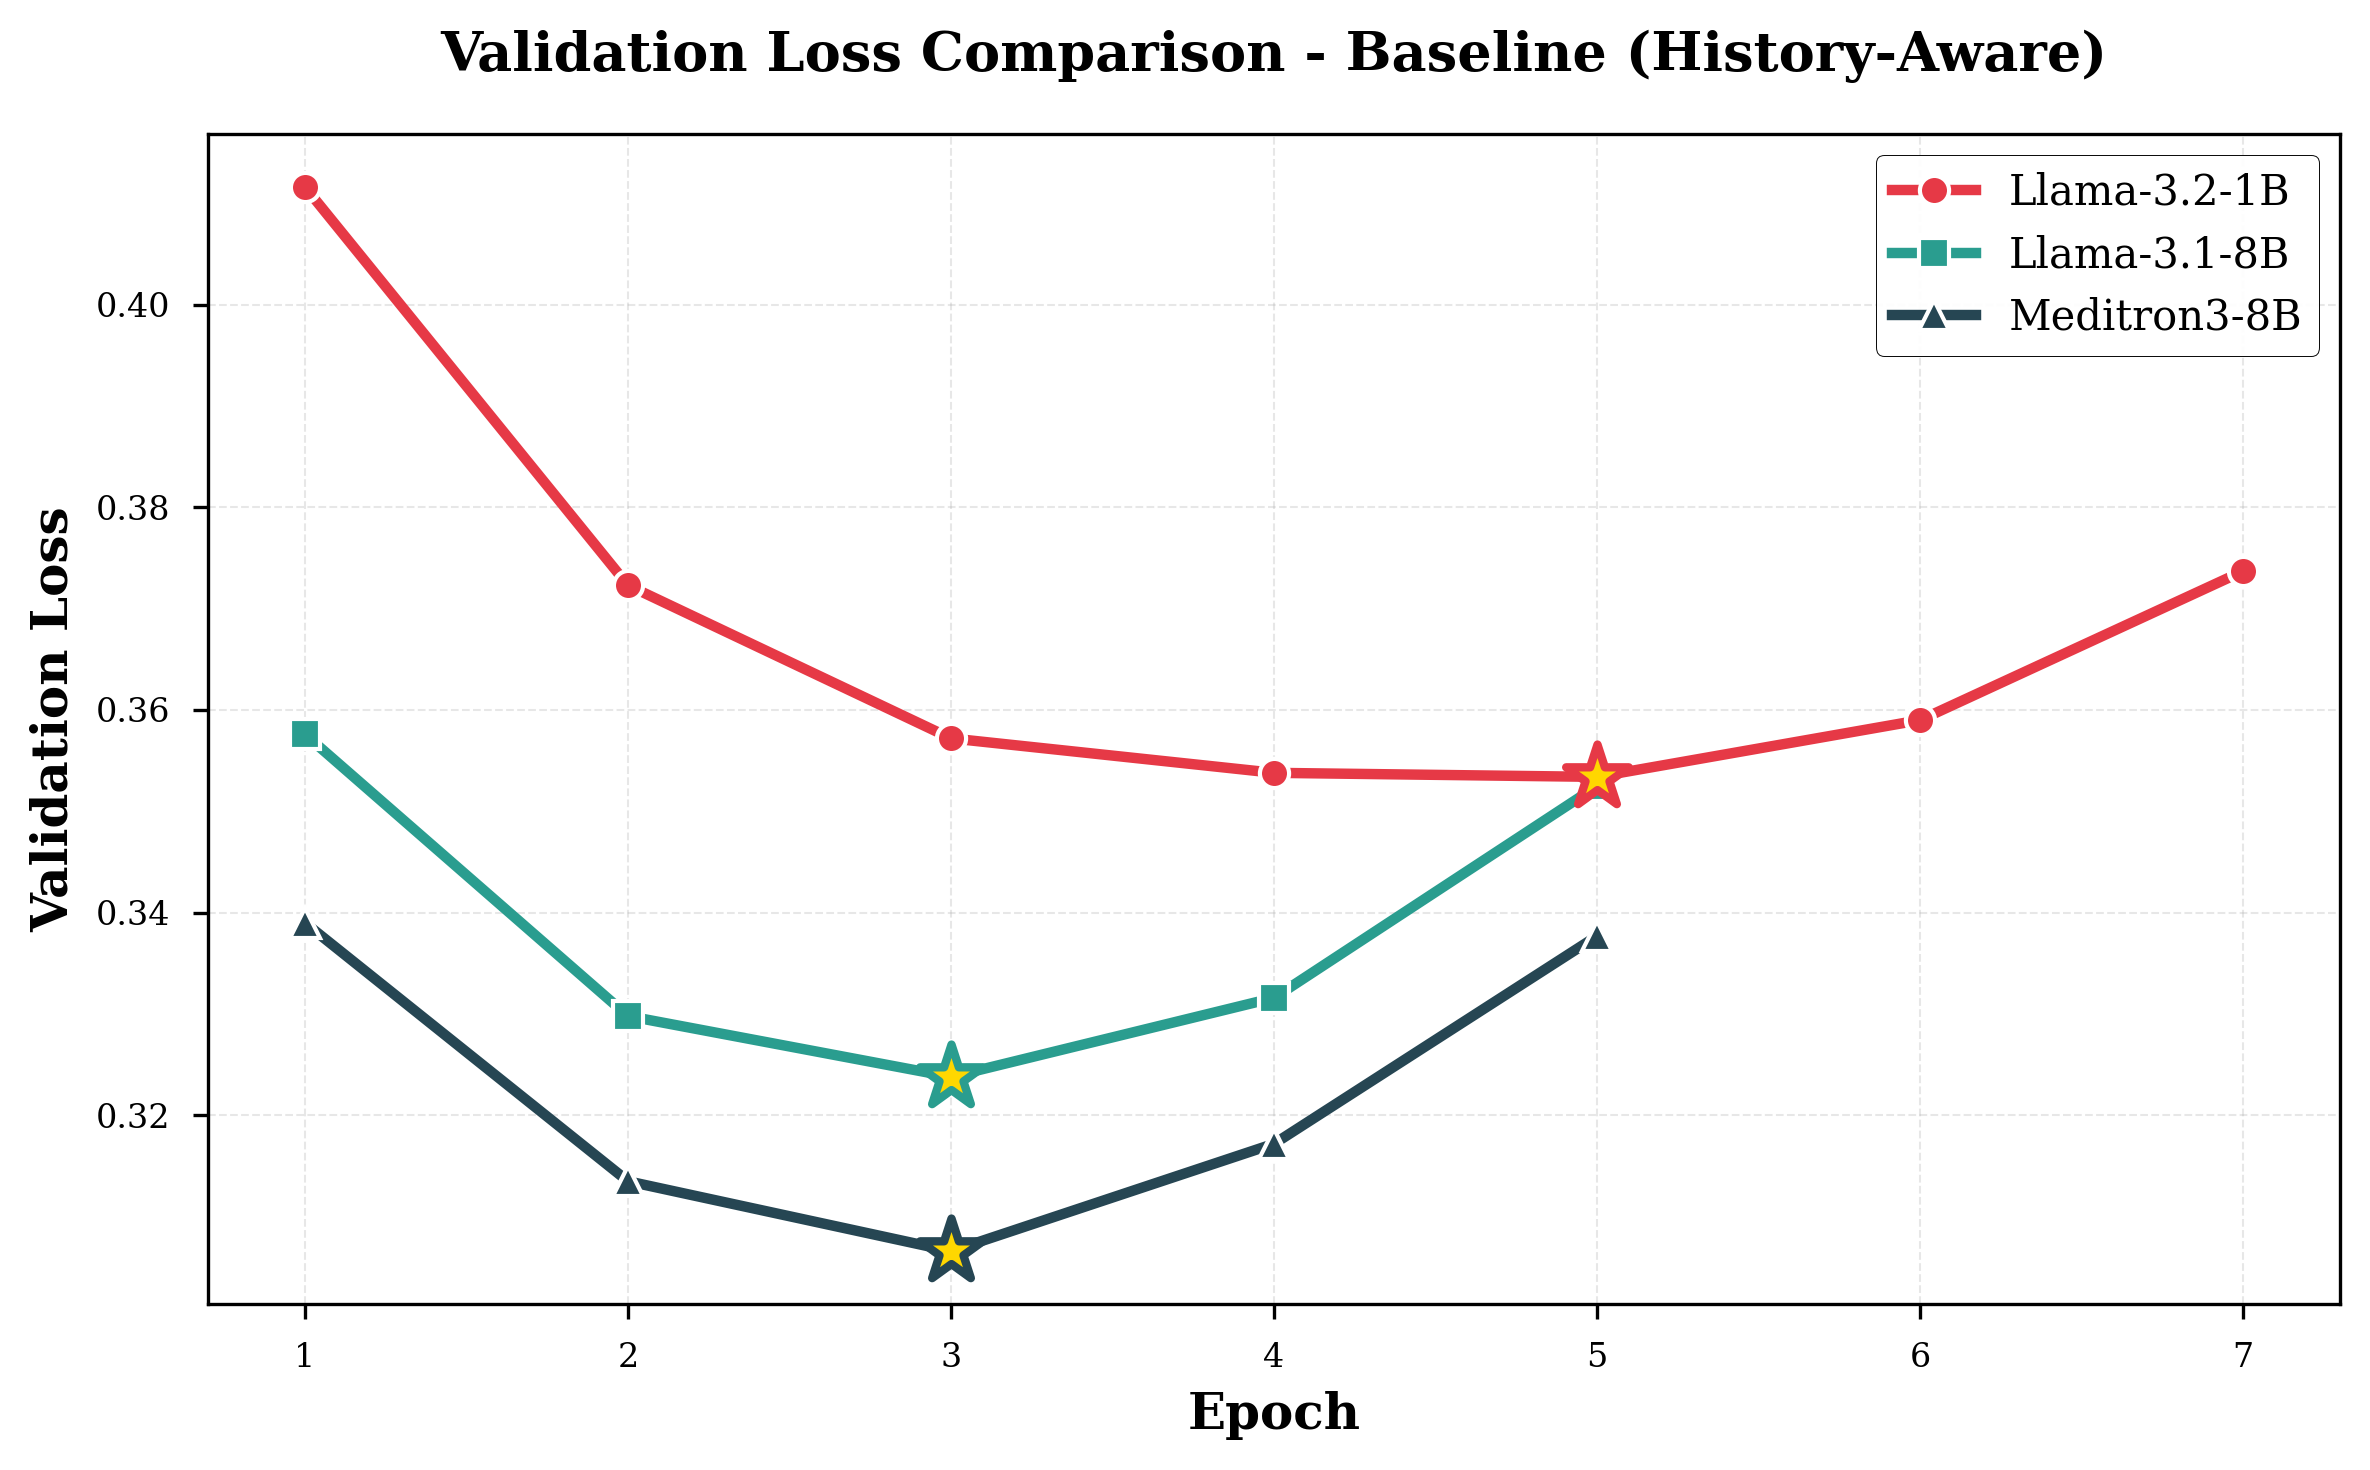
\includegraphics[width=\linewidth]{Images/validation_loss_comparison_history.png}
%         \caption{Val loss comparison}
%         \label{fig:task2-textgen-val-loss-comparison}
%     \end{subfigure}
%     \caption{Task~2 (next-visit diagnosis prediction), Textgen pipeline. Training and validation loss across epochs for each backbone model.}
%     \label{fig:task2-textgen-training}
% \end{figure}

% \subsection{Optimisation and Regularisation}
% \label{subsec:optim}

% Both architectures are trained using the AdamW optimiser~\cite{loshchilov2019decoupled} with a learning rate of \(2 \times 10^{-4}\) and zero weight decay on the LoRA parameters. The effective batch size is set by using a per-device batch size of one sequence and accumulating gradients over multiple optimisation steps, yielding an effective batch size of 16 multimodal prompts. A short warmup phase covers approximately \(3\%\) of the total training steps, followed by a linear decay schedule.

% Models are typically trained for 4--6 epochs, depending on the architecture and dataset size (with fewer epochs for Textgen due to the heavier supervision signal in natural language). Gradient checkpointing is enabled throughout to reduce the memory footprint of backpropagation in the Transformer backbone. Computations are performed in FP16 on older GPUs and BF16 on more recent architectures that natively support it.

% \subsection{Training Dynamics and Logging}
% \label{subsec:training-dynamics}

% To monitor training dynamics, both pipelines record:

% \begin{itemize}
%     \item per-step training loss and learning rate,
%     \item epoch-level averages of training loss,
%     \item validation loss and a derived perplexity estimate on the validation set.
% \end{itemize}

% A lightweight callback mechanism aggregates per-step metrics into compact epoch summaries printed to the log. These summaries provide a quick overview of convergence behaviour without overwhelming the log files.

% For Textgen, an additional safeguard is implemented to handle rare edge cases in which, due to aggressive truncation of long notes, all tokens in a batch correspond to the prompt and none to the supervised output. In this case, a zero loss is returned for that batch instead of raising an error, ensuring that occasional pathological examples do not halt training.

% \subsection{Distributed Training and Stability}
% \label{subsec:stability}

% Textgen is designed to support multi-GPU training via distributed data parallelism. To this end, several practical tweaks are employed:

% \begin{itemize}
%     \item communication backend settings (e.g.\ NCCL timeouts and interface whitelists) are configured via environment variables to reduce the risk of deadlocks,
%     \item data loading uses a small number of worker processes and conservative pinning options to avoid resource contention,
%     \item at the end of training, a dedicated cleanup routine synchronises all devices, attempts a final barrier across processes, and explicitly tears down the distributed process group before releasing GPU memory.
% \end{itemize}

% These measures proved important in avoiding occasional training hangs that can arise when long-running distributed jobs terminate unexpectedly.

% \subsection{Early Stopping and Model Selection}
% \label{subsec:early-stop}

% Both models use early stopping based on validation loss. After each epoch, the model is evaluated on the validation set, and the epoch-level validation loss is recorded. If no improvement is observed over two consecutive evaluations, training is stopped early to prevent overfitting and unnecessary computation. The checkpoint with the lowest validation loss is retained as the final model for testing.

% For Codegen, the retained state consists of the adapter parameters and tokenizer configuration, saved alongside a JSON representation of the label vocabulary. For Textgen, the LoRA adapter, tokenizer, and any additional artefacts required by the semantic mapping layer are stored for later inference and analysis.

% \subsection{Inference Configuration}
% \label{subsec:decoding}

% At inference time, both pipelines use constrained decoding strategies tailored to their outputs.

% For Codegen, generation is run over the full multimodal prompt with a fixed maximum number of new tokens, usually using greedy decoding or beam search with a small beam size. The generated continuation after the dedicated code marker is parsed into a list of candidate ICD-9 codes, which are normalised, de-duplicated, and filtered to remove obviously ill-formed codes.

% For Textgen, the model generates a short list of diagnosis phrases using either greedy decoding or beam search. The raw text is post-processed into individual diagnostic statements by splitting on line breaks and stripping bullet markers. These phrases are then passed to the semantic mapping layer (Section~\ref{subsec:textgen-arch}), which retrieves and ranks ICD-9 codes based on semantic similarity.

\section{Training Procedure and Implementation Details}
\label{sec:training}

This section summarises the optimisation setup, checkpointing strategy, and practical stability measures used to fine-tune Codegen and Textgen (Section~\ref{sec:model-architectures}) on the multimodal EHR datasets.

\paragraph{Implementation and experiment scope.}
All models are implemented using the Hugging Face \texttt{transformers} ecosystem~\cite{wolf2020transformers} with parameter-efficient fine-tuning via LoRA~\cite{hu2021lora}. Experiments use decoder-only backbones from the LLaMA and Meditron families: \texttt{Llama-3.2-1B-Instruct}, \texttt{Llama-3.1-8B-Instruct}, and \texttt{Meditron-8B}~\cite{touvron2023llama,chen2023meditron}. For Task~1, we train both pipelines (Codegen and Textgen) across all three backbones. For Task~2, we train only Textgen (again across all three backbones), since Task~1 results establish Textgen as the stronger pipeline and longitudinal prediction relies heavily on robust narrative understanding and semantic normalisation.

\paragraph{Optimisation and regularisation.}
All models are fine-tuned with AdamW~\cite{loshchilov2019decoupled}. We use a learning rate of $2\times 10^{-4}$ for the trainable LoRA parameters, with zero weight decay on the adapters. Due to long prompts, the per-device batch size is set to one sequence and gradients are accumulated to achieve an effective batch size of 16 admissions per optimisation step. We apply a short warm-up phase (approximately $3\%$ of total steps) followed by a linear learning-rate decay. Gradient checkpointing is enabled to reduce activation memory, and training runs in mixed precision (FP16 or BF16 depending on GPU support). Models are typically trained for 4--6 epochs (dataset- and backbone-dependent), with early stopping based on validation loss.

\paragraph{Supervision masking and truncation safeguards.}
Both pipelines are trained as causal language models with loss applied only to the supervised output region: prompt tokens are masked out, and cross-entropy is computed over the target continuation (ICD-9 codes for Codegen; diagnosis terms for Textgen). A maximum sequence length is enforced; if an example exceeds the limit it is truncated. For Textgen, we implement a safeguard for rare truncation edge cases where the supervised target is fully removed (i.e., a batch contains only prompt tokens). In such cases the step returns a zero loss rather than raising an exception, preventing occasional pathological samples from interrupting training.

\paragraph{Training dynamics and model selection.}
During fine-tuning we log step-level training loss and learning rate, and compute epoch-level summaries including validation loss after each epoch (The epoch level logs are available in the Appendix \ref{sec:appendix} for both pipelines). We retain the checkpoint with the lowest validation loss and apply early stopping if validation loss fails to improve for two consecutive epochs. Representative training and validation loss curves for Task~1 and Task~2 are shown in Figures~\ref{fig:task1-codegen-training}--\ref{fig:task2-textgen-training}; predictive performance is reported in Chapter~\ref{sec:results}.

\begin{figure}[t]
    \centering
    \begin{subfigure}{0.32\textwidth}
        \centering
        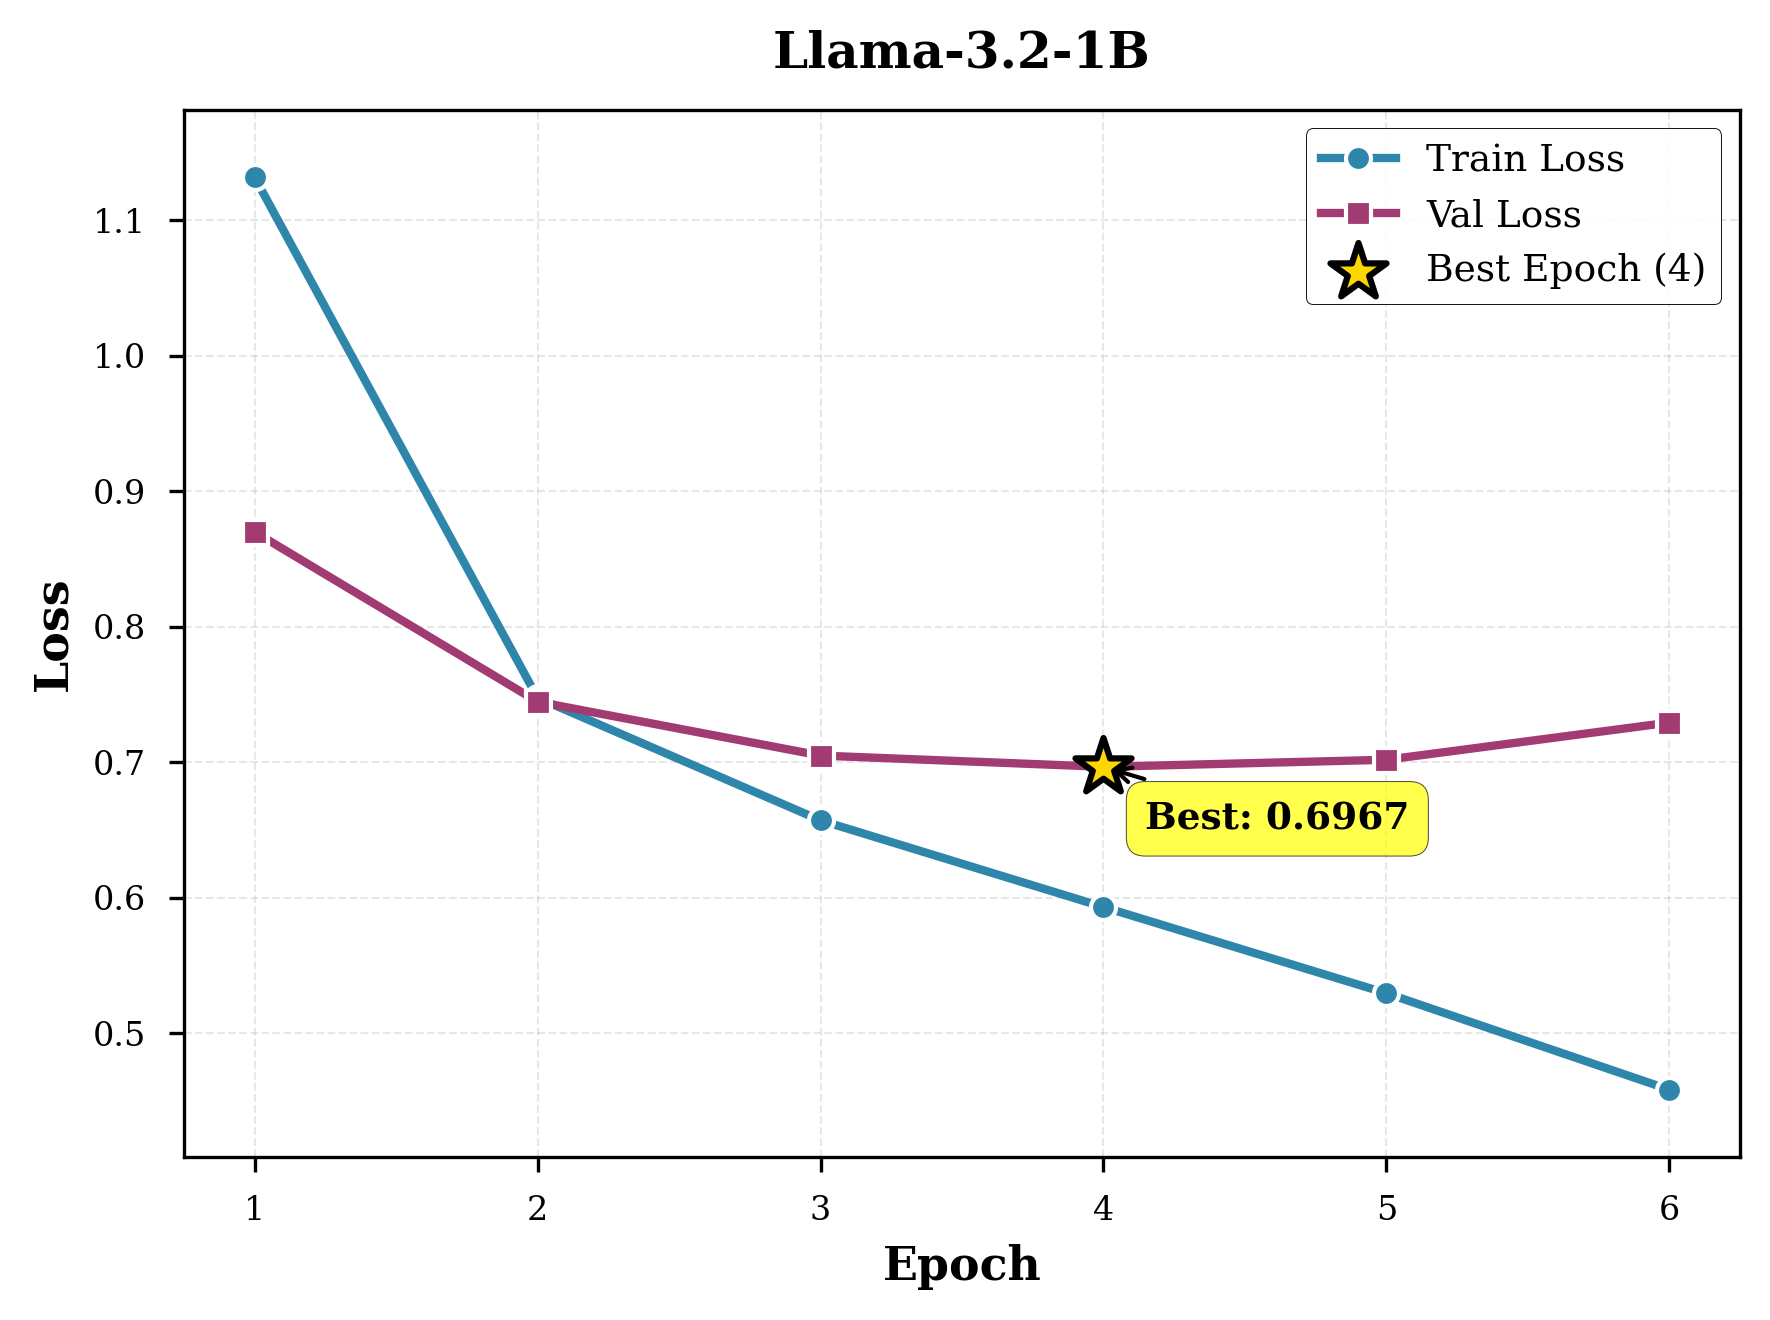
\includegraphics[width=\linewidth]{Images/codegen_training/training_curve_llama_32_1b.png}
        \caption{Codegen -- Llama-3.2-1B}
        \label{fig:task1-codegen-llama1b}
    \end{subfigure}\hfill
    \begin{subfigure}{0.32\textwidth}
        \centering
        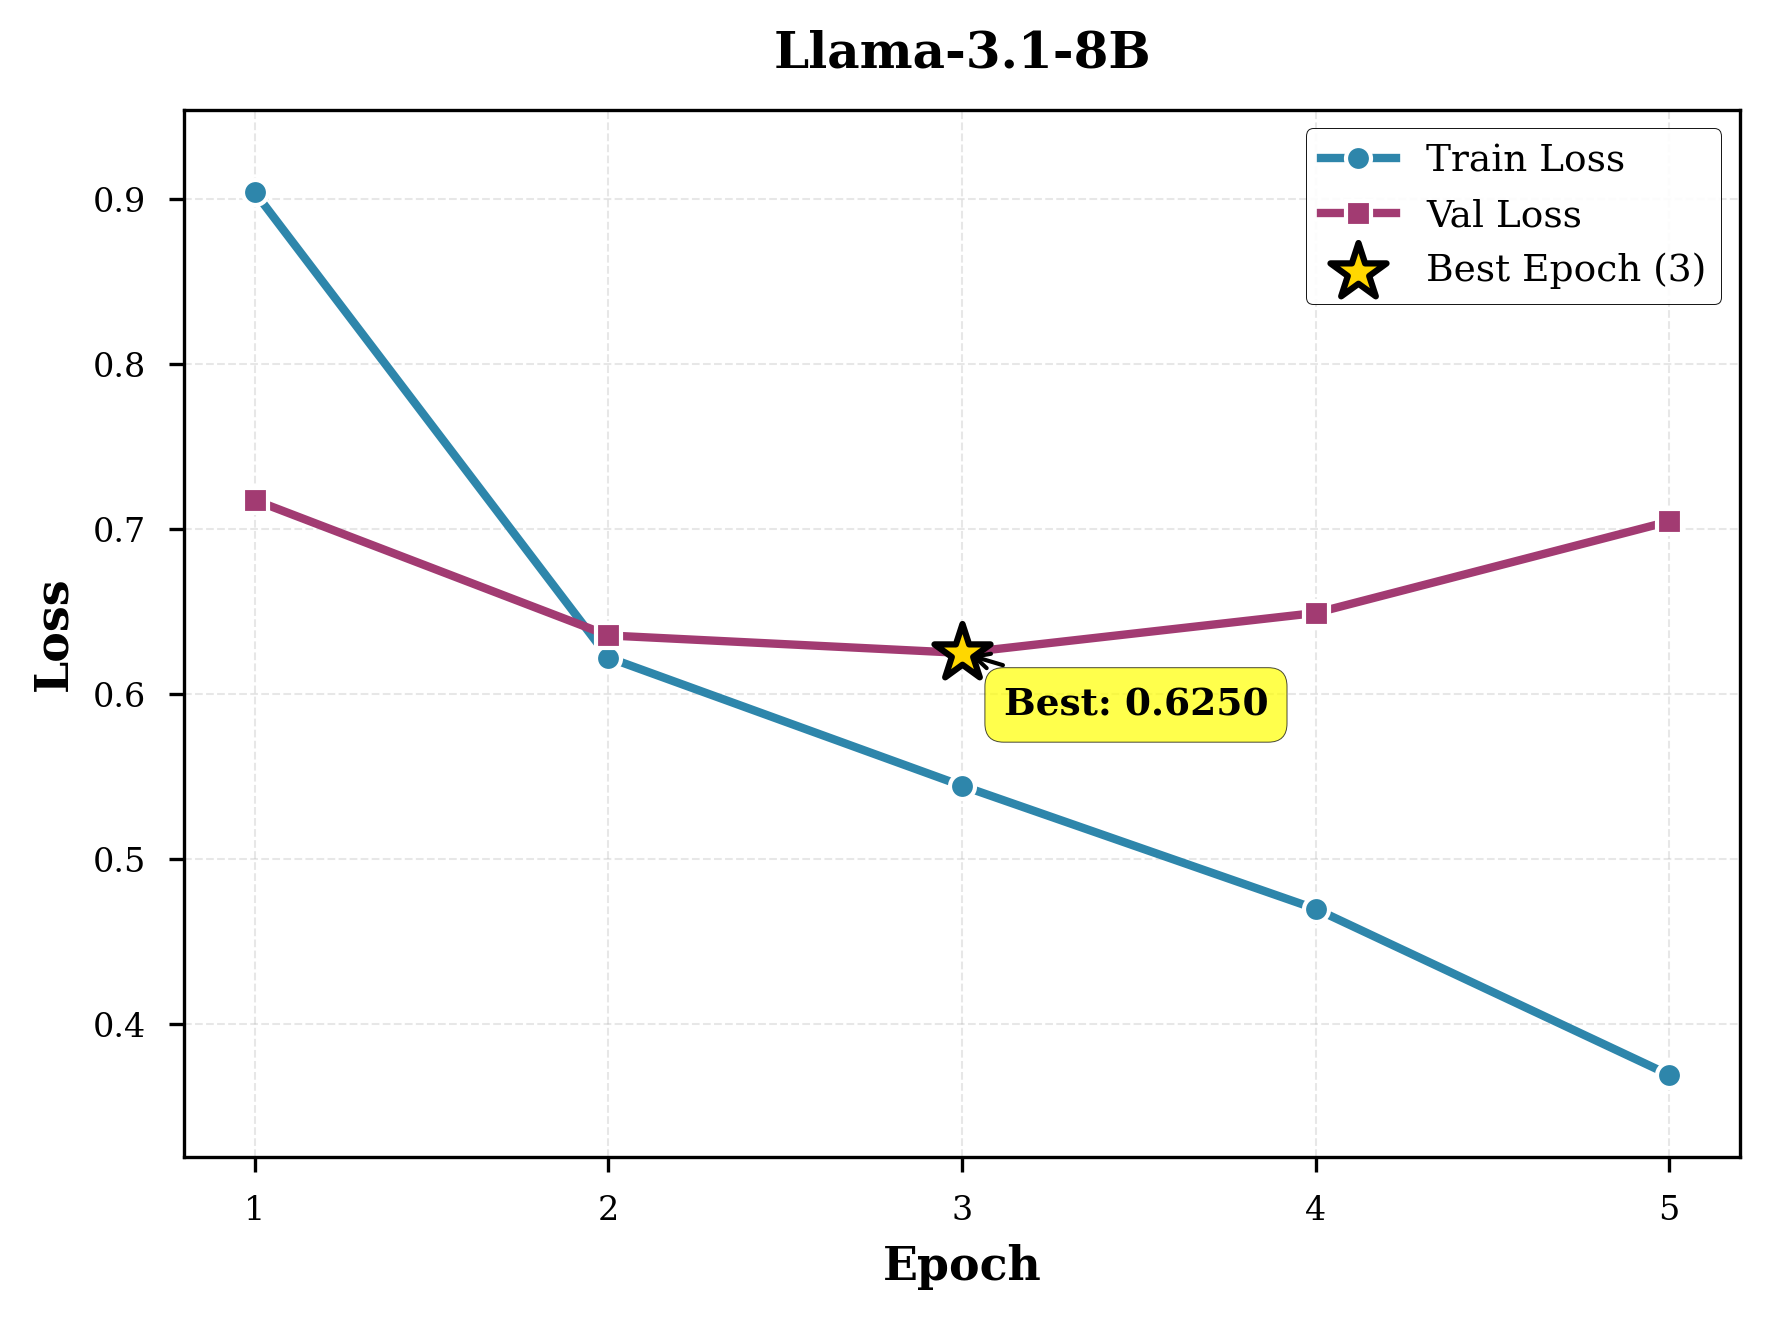
\includegraphics[width=\linewidth]{Images/codegen_training/training_curve_llama_31_8b.png}
        \caption{Codegen -- Llama-3.1-8B}
        \label{fig:task1-codegen-llama8b}
    \end{subfigure}\hfill
    \begin{subfigure}{0.32\textwidth}
        \centering
        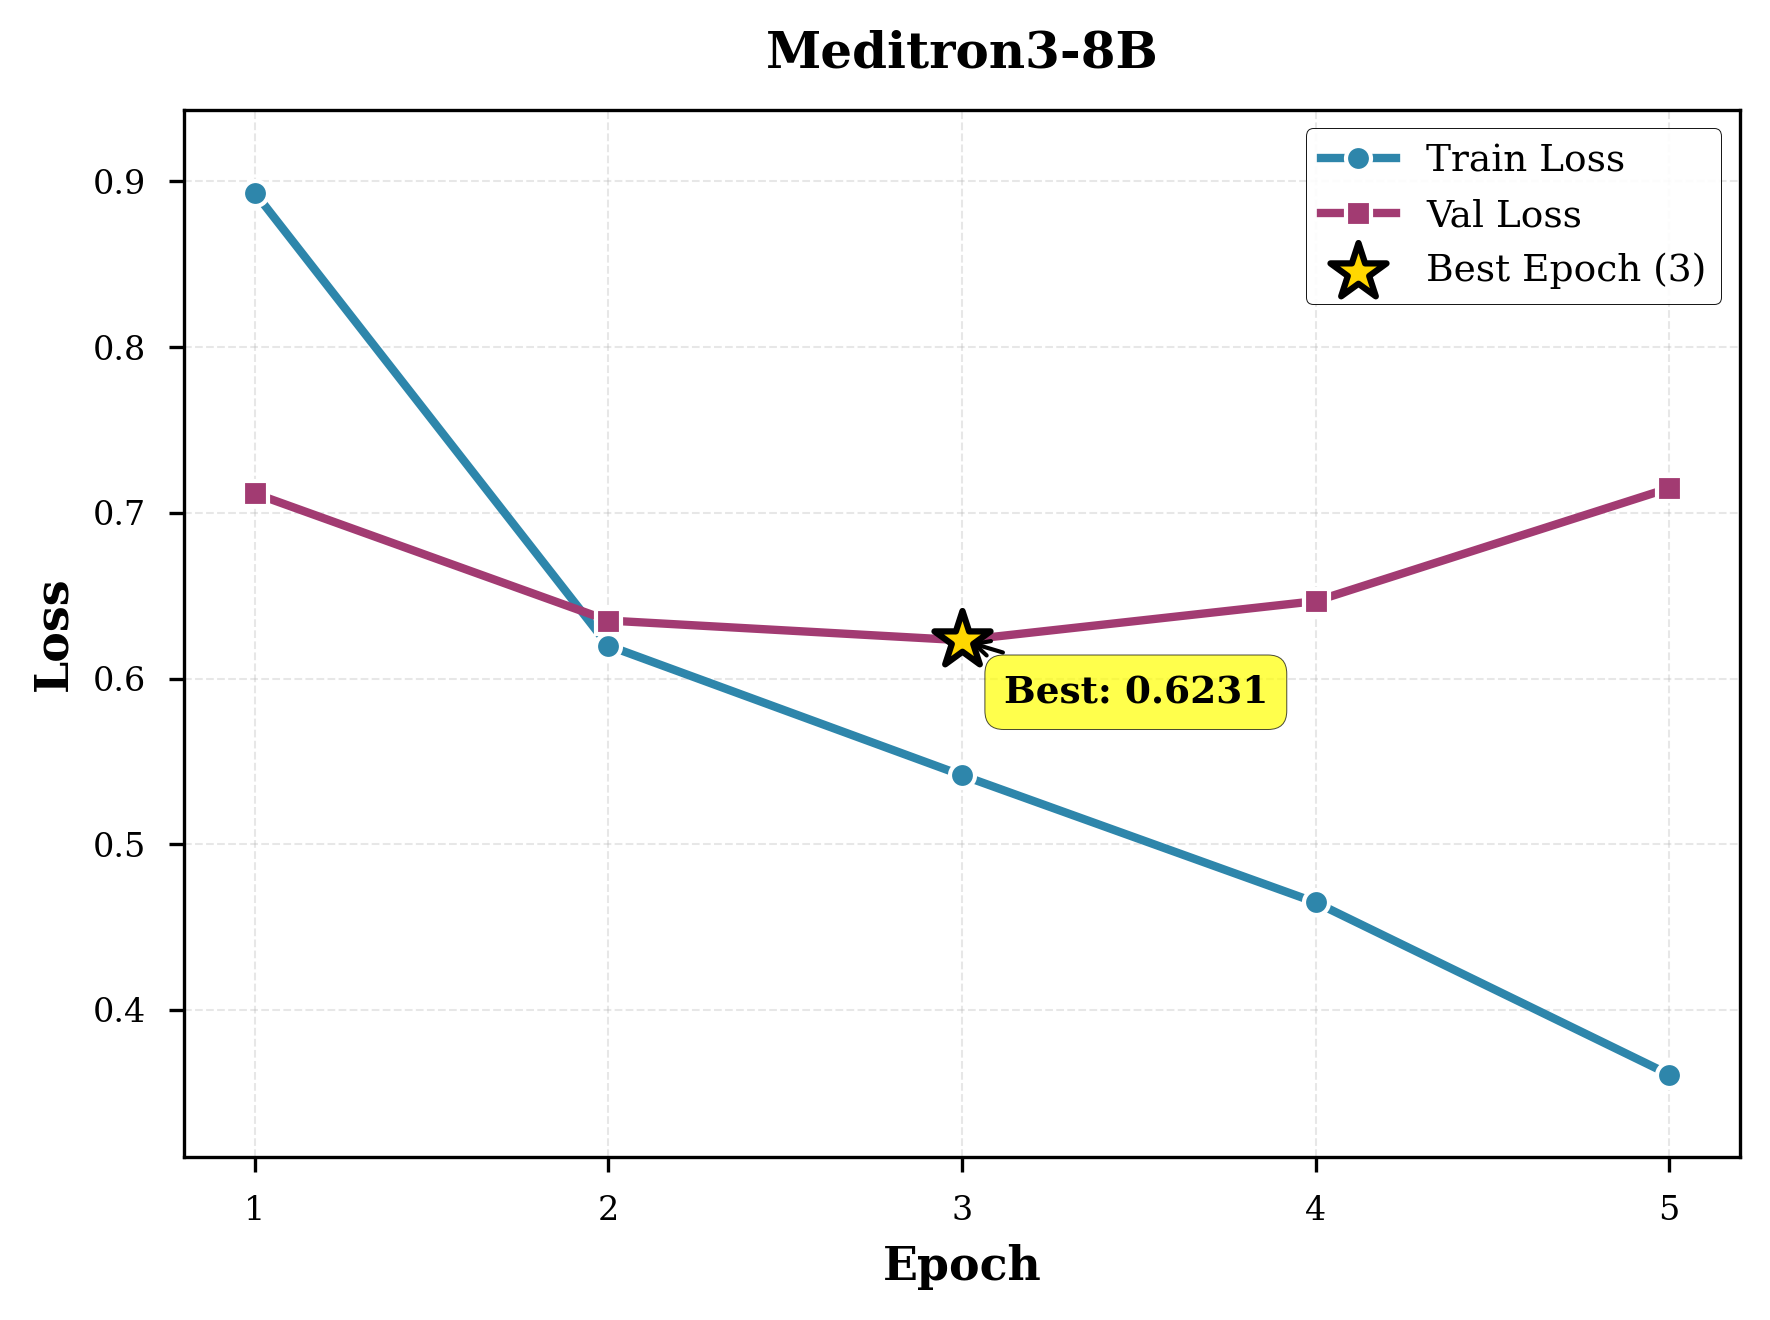
\includegraphics[width=\linewidth]{Images/codegen_training/training_curve_meditron3_8b.png}
        \caption{Codegen -- Meditron-8B}
        \label{fig:task1-codegen-meditron8b}
    \end{subfigure}
    \caption{Task~1 (current-visit diagnosis prediction), Codegen pipeline. Training and validation loss across epochs for each backbone model.}
    \label{fig:task1-codegen-training}
\end{figure}

\begin{figure}[t]
    \centering
    \begin{subfigure}{0.5\textwidth}
        \centering
        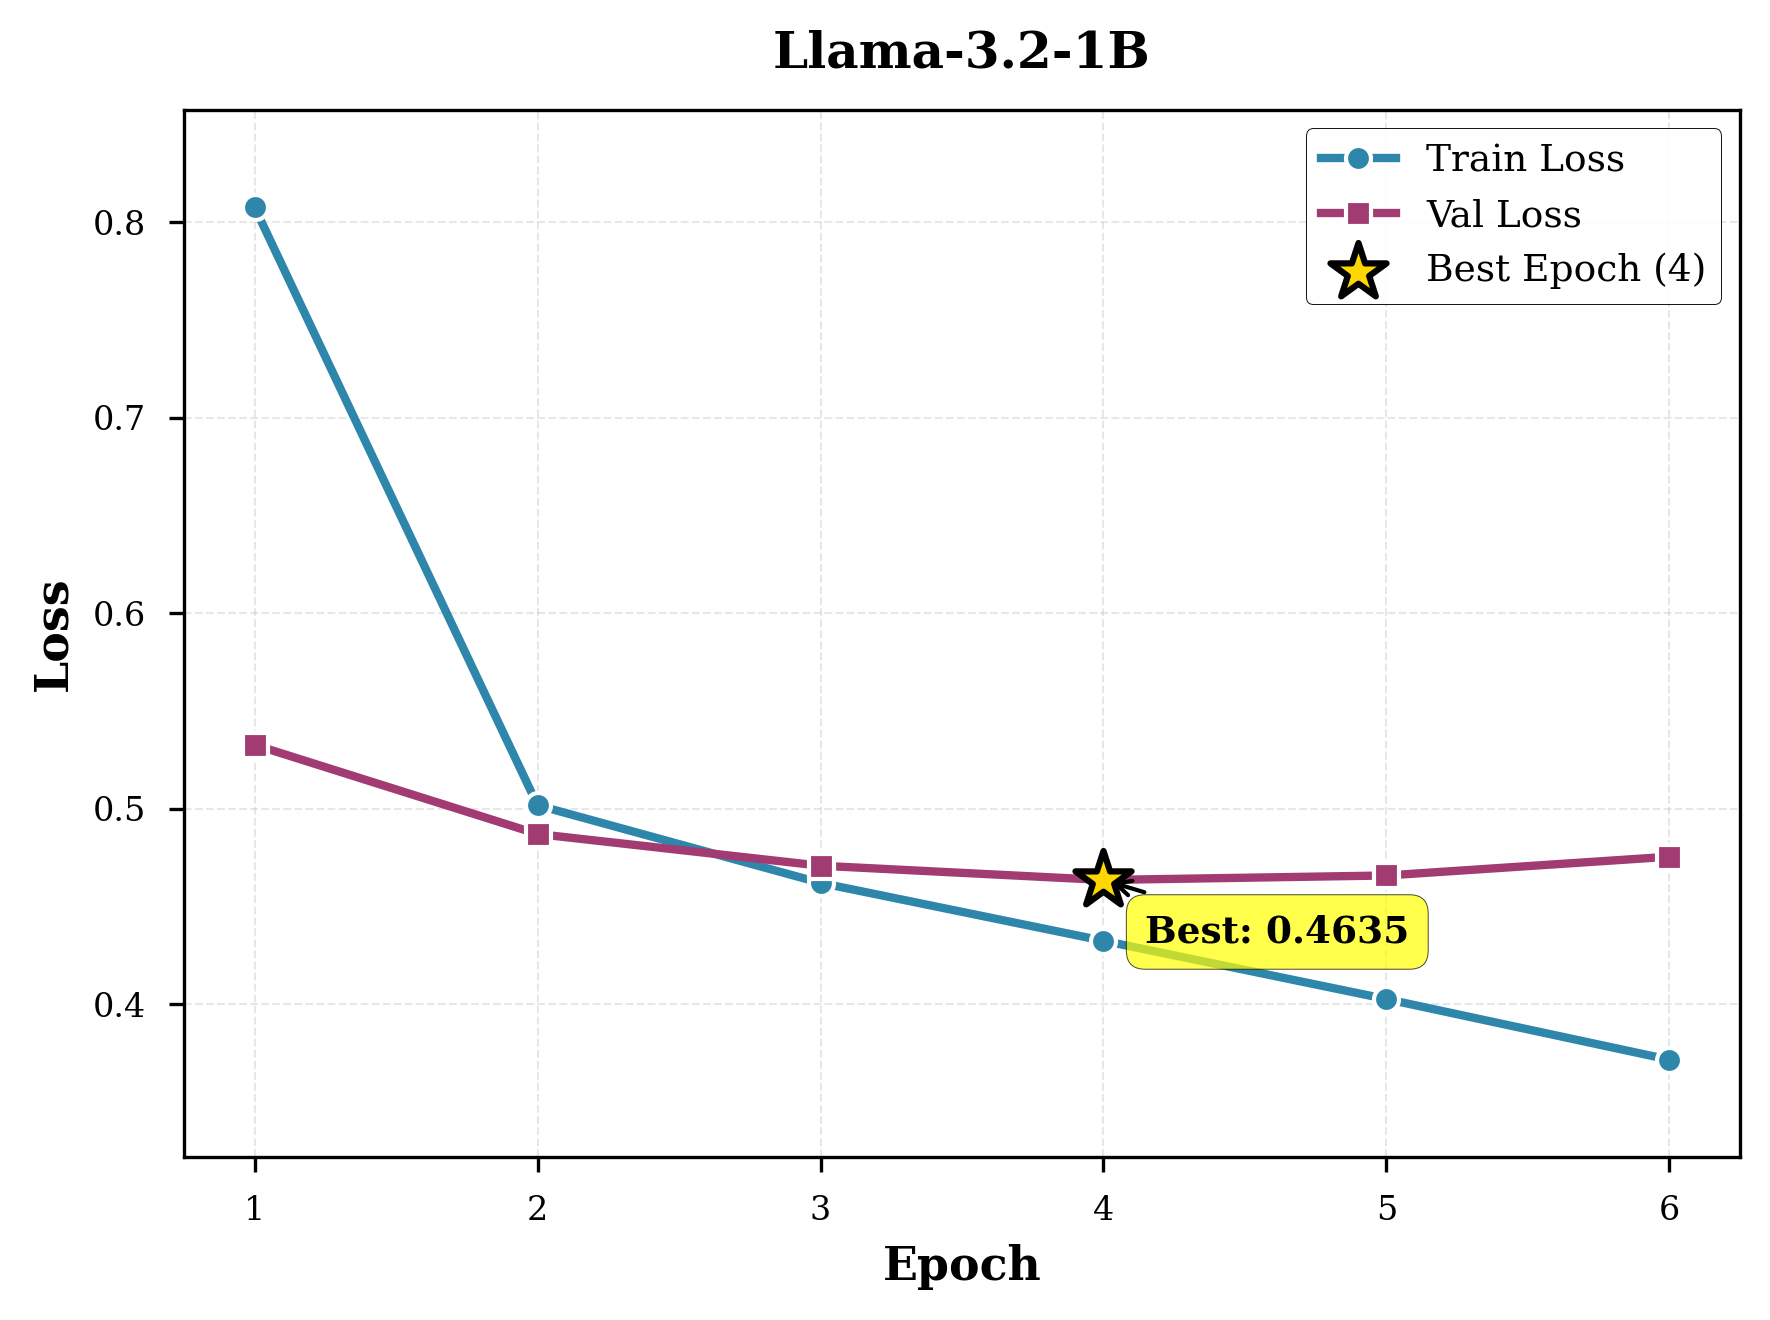
\includegraphics[width=\linewidth]{Images/training_curve_llama_32_1b.png}
        \caption{Textgen -- Llama-3.2-1B}
        \label{fig:task1-textgen-llama1b}
    \end{subfigure}\hfill
    \begin{subfigure}{0.5\textwidth}
        \centering
        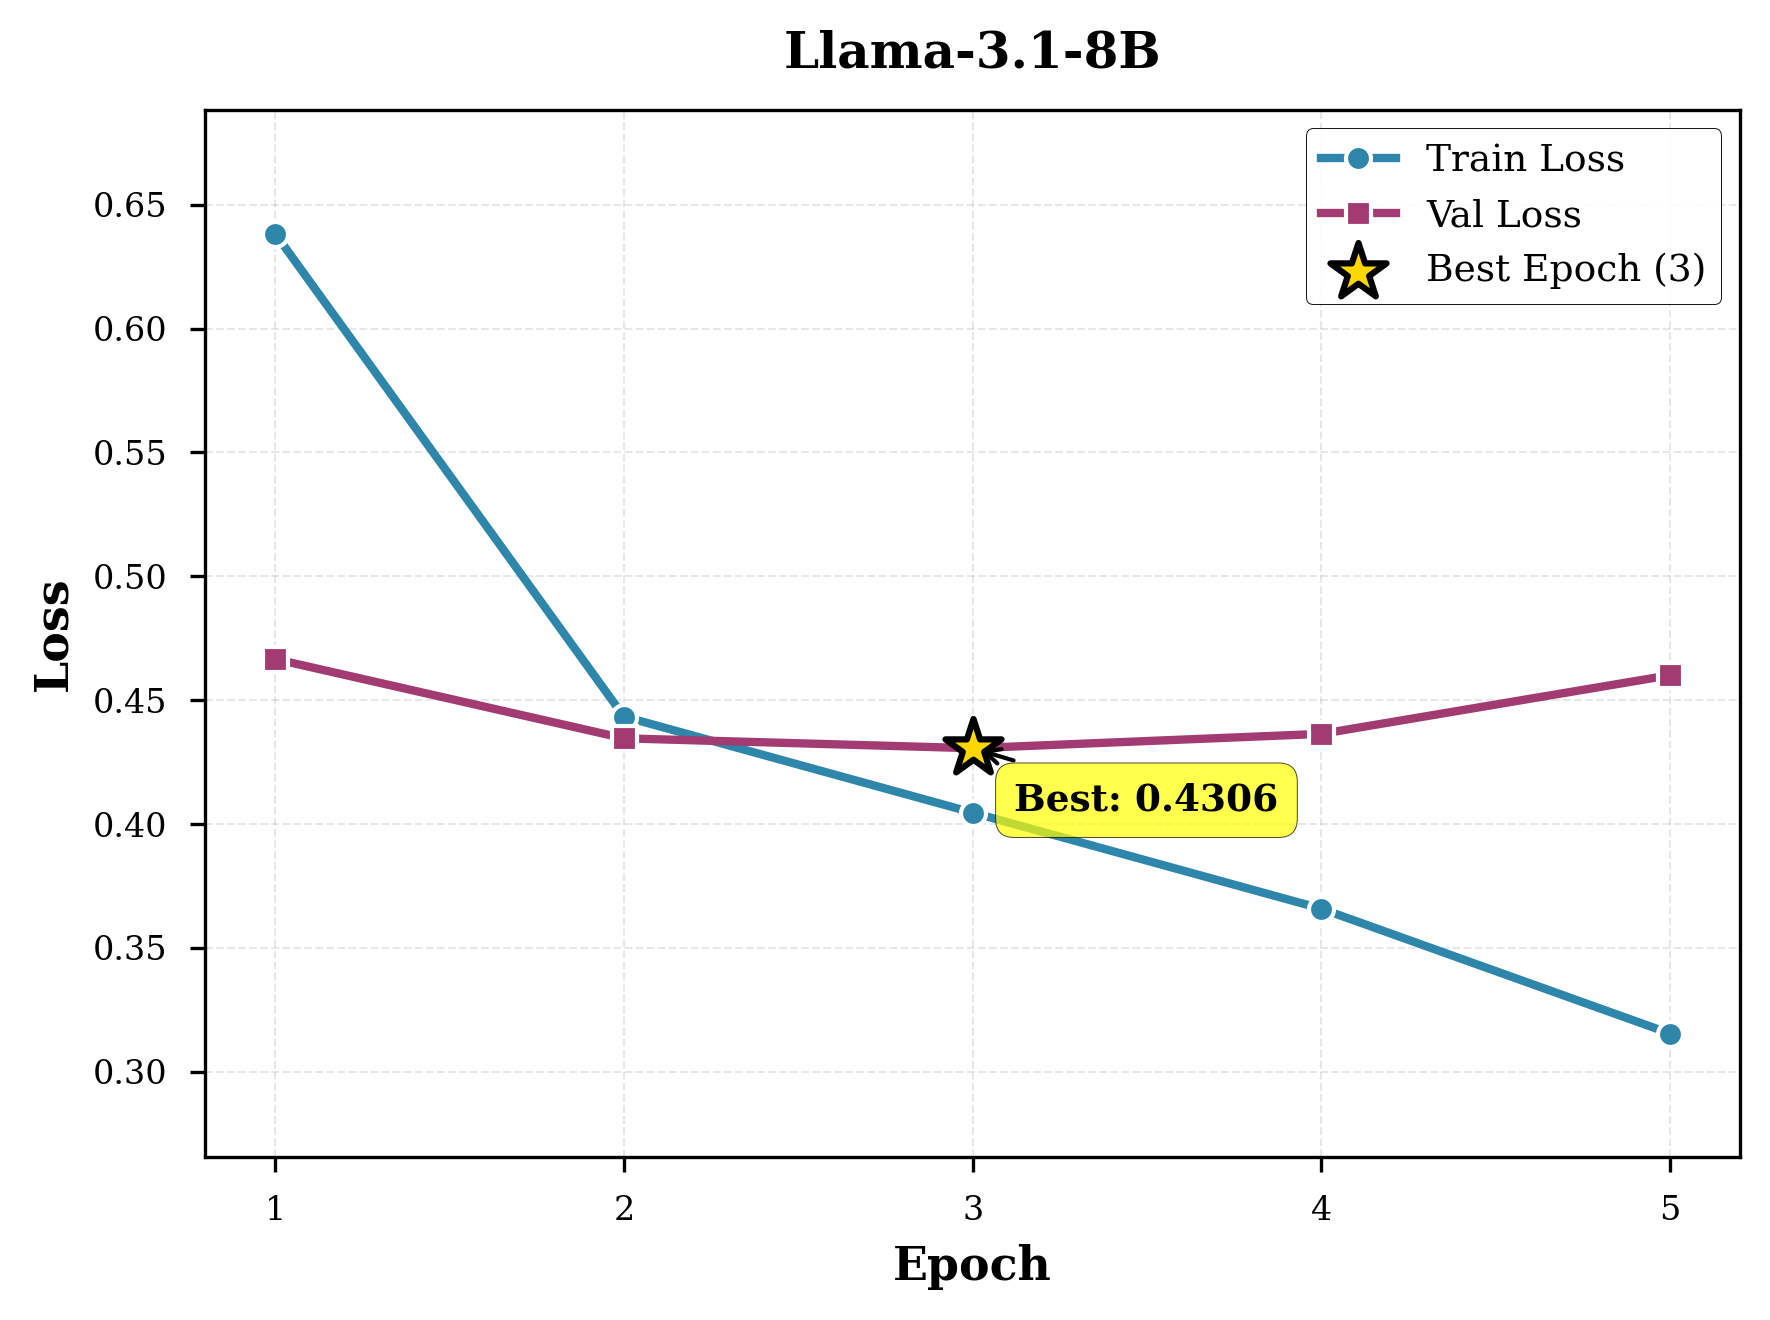
\includegraphics[width=\linewidth]{Images/training_curve_llama_31_8b.png}
        \caption{Textgen -- Llama-3.1-8B}
        \label{fig:task1-textgen-llama8b}
    \end{subfigure}\hfill
    \begin{subfigure}{0.5\textwidth}
        \centering
        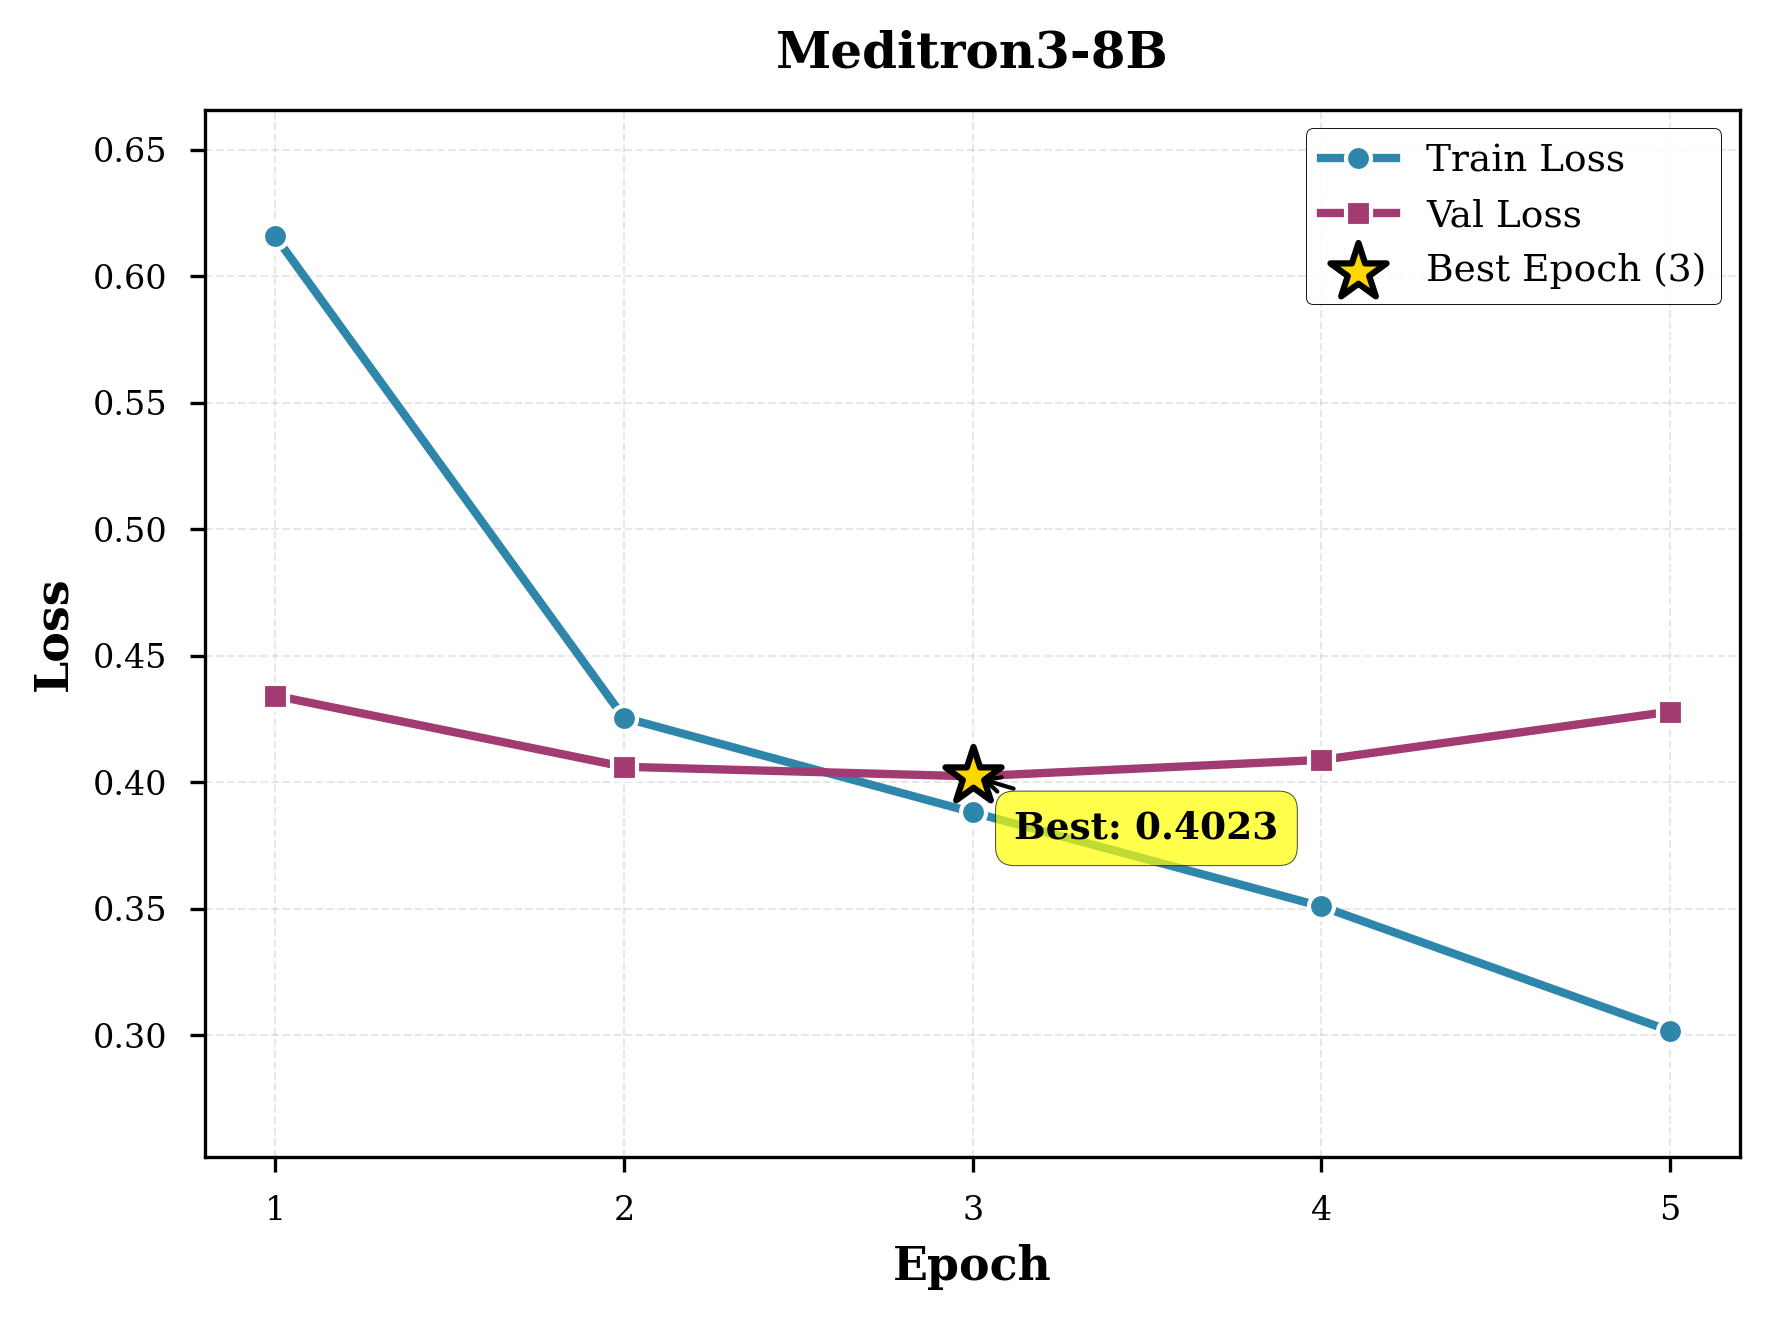
\includegraphics[width=\linewidth]{Images/training_curve_meditron3_8b.png}
        \caption{Textgen -- Meditron-8B}
        \label{fig:task1-textgen-meditron8b}
    \end{subfigure}
    \begin{subfigure}{0.5\textwidth}
        \centering
        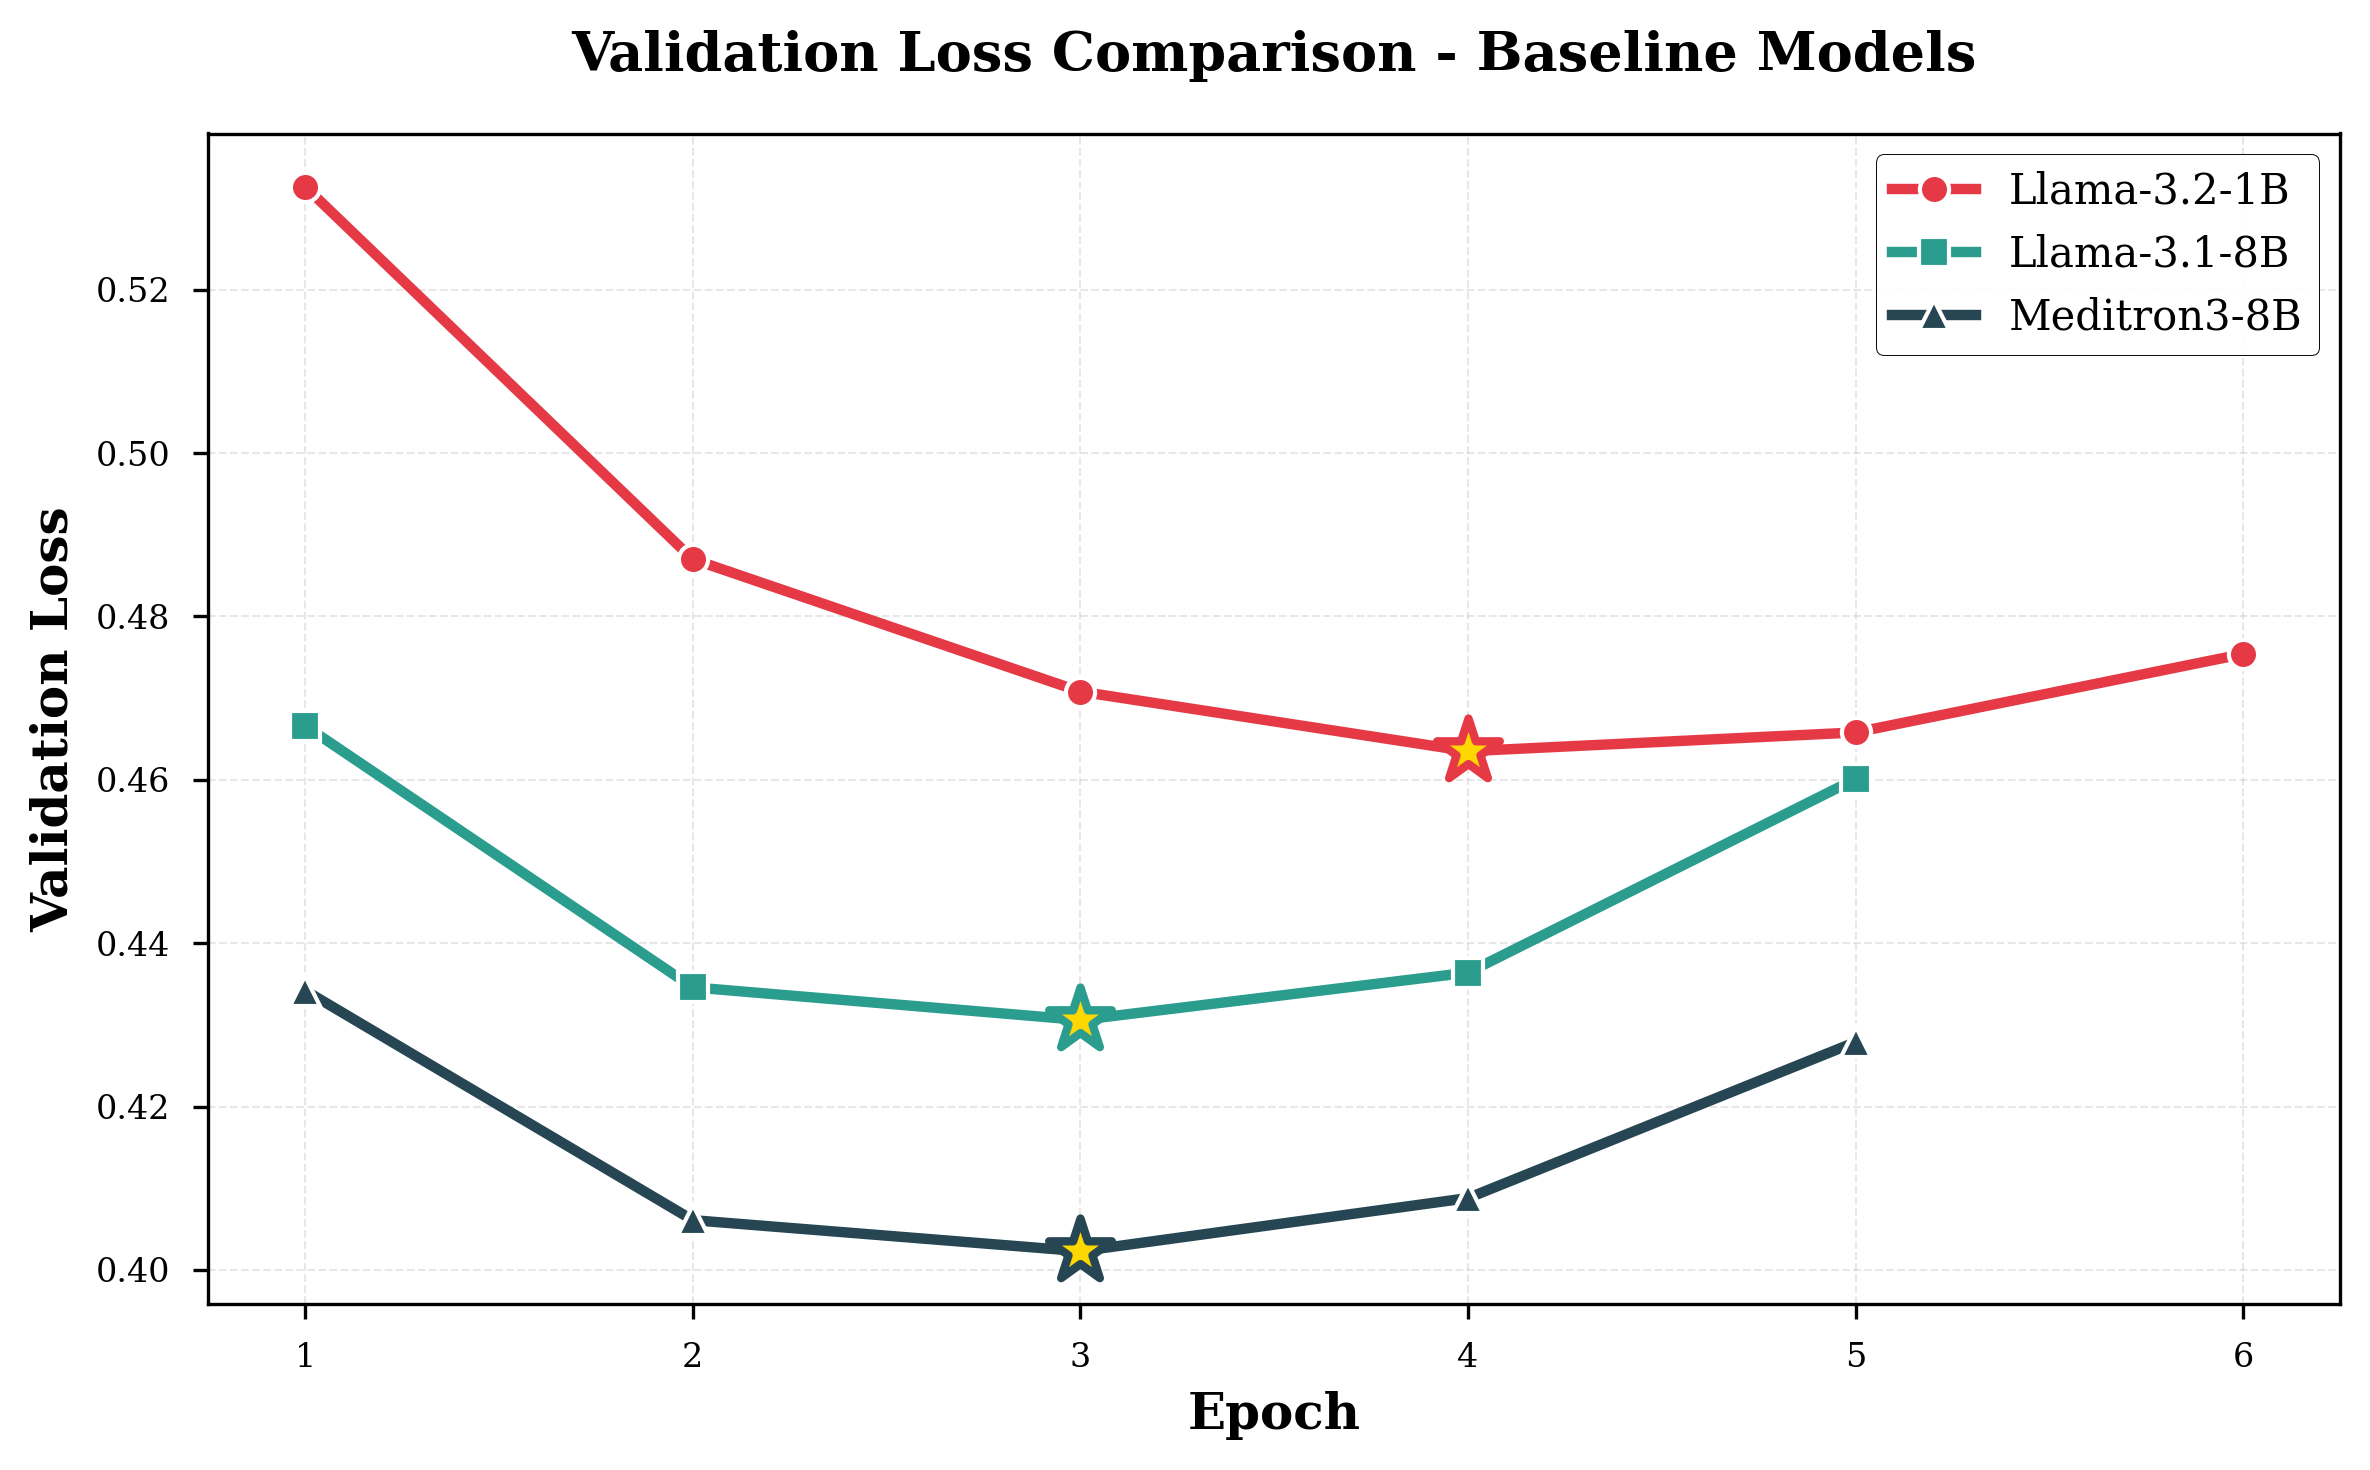
\includegraphics[width=\linewidth]{Images/validation_loss_comparison.png}
        \caption{Validation loss comparison}
        \label{fig:task1-textgen-val-loss-comparison}
    \end{subfigure}
    \caption{Task~1 (current-visit diagnosis prediction), Textgen pipeline. Training and validation loss across epochs for each backbone model.}
    \label{fig:task1-textgen-training}
\end{figure}

\begin{figure}[t]
    \centering
    \begin{subfigure}{0.5\textwidth}
        \centering
        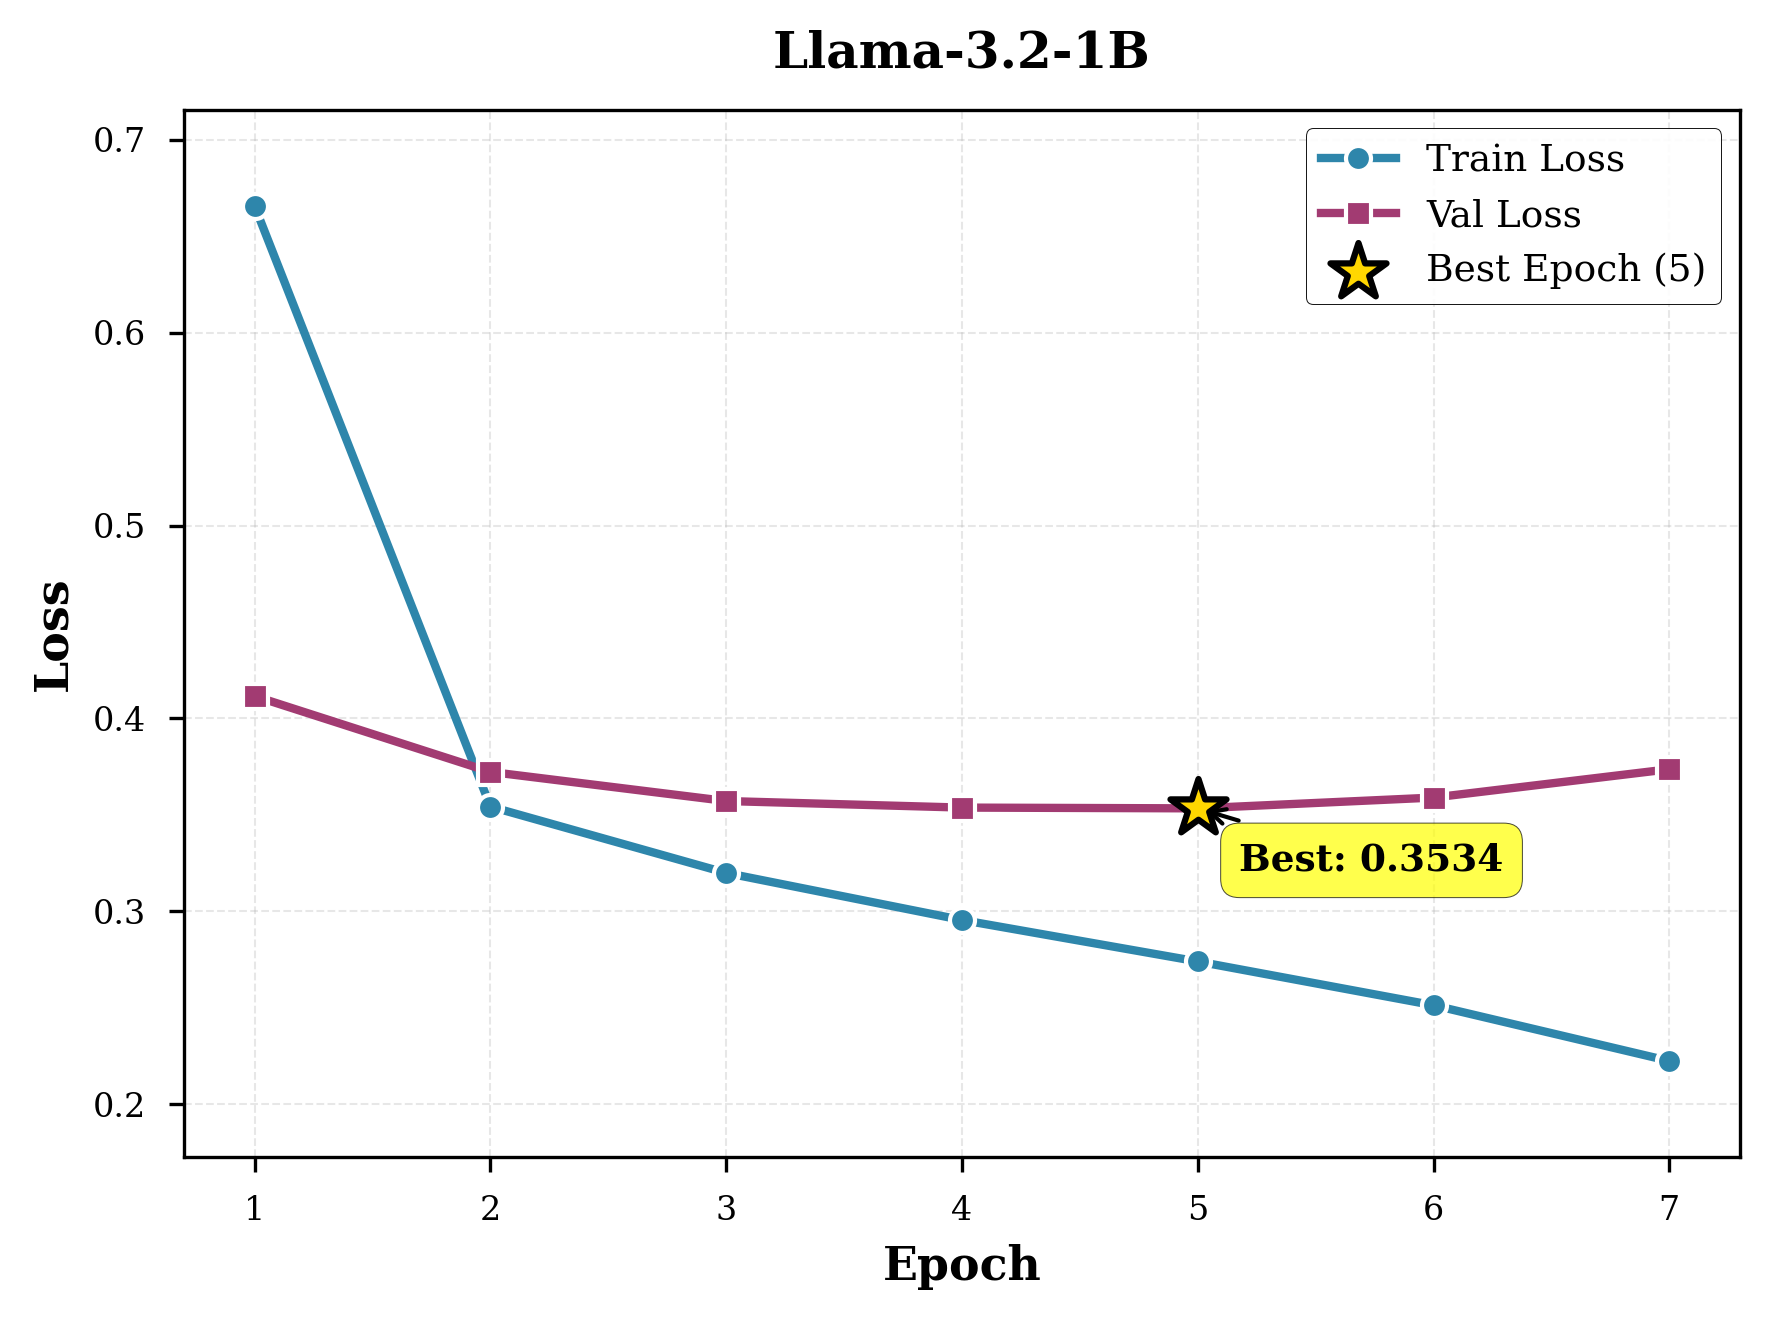
\includegraphics[width=\linewidth]{Images/training_curve_history_llama_32_1b.png}
        \caption{Textgen -- Llama-3.2-1B}
        \label{fig:task2-textgen-llama1b}
    \end{subfigure}\hfill
    \begin{subfigure}{0.5\textwidth}
        \centering
        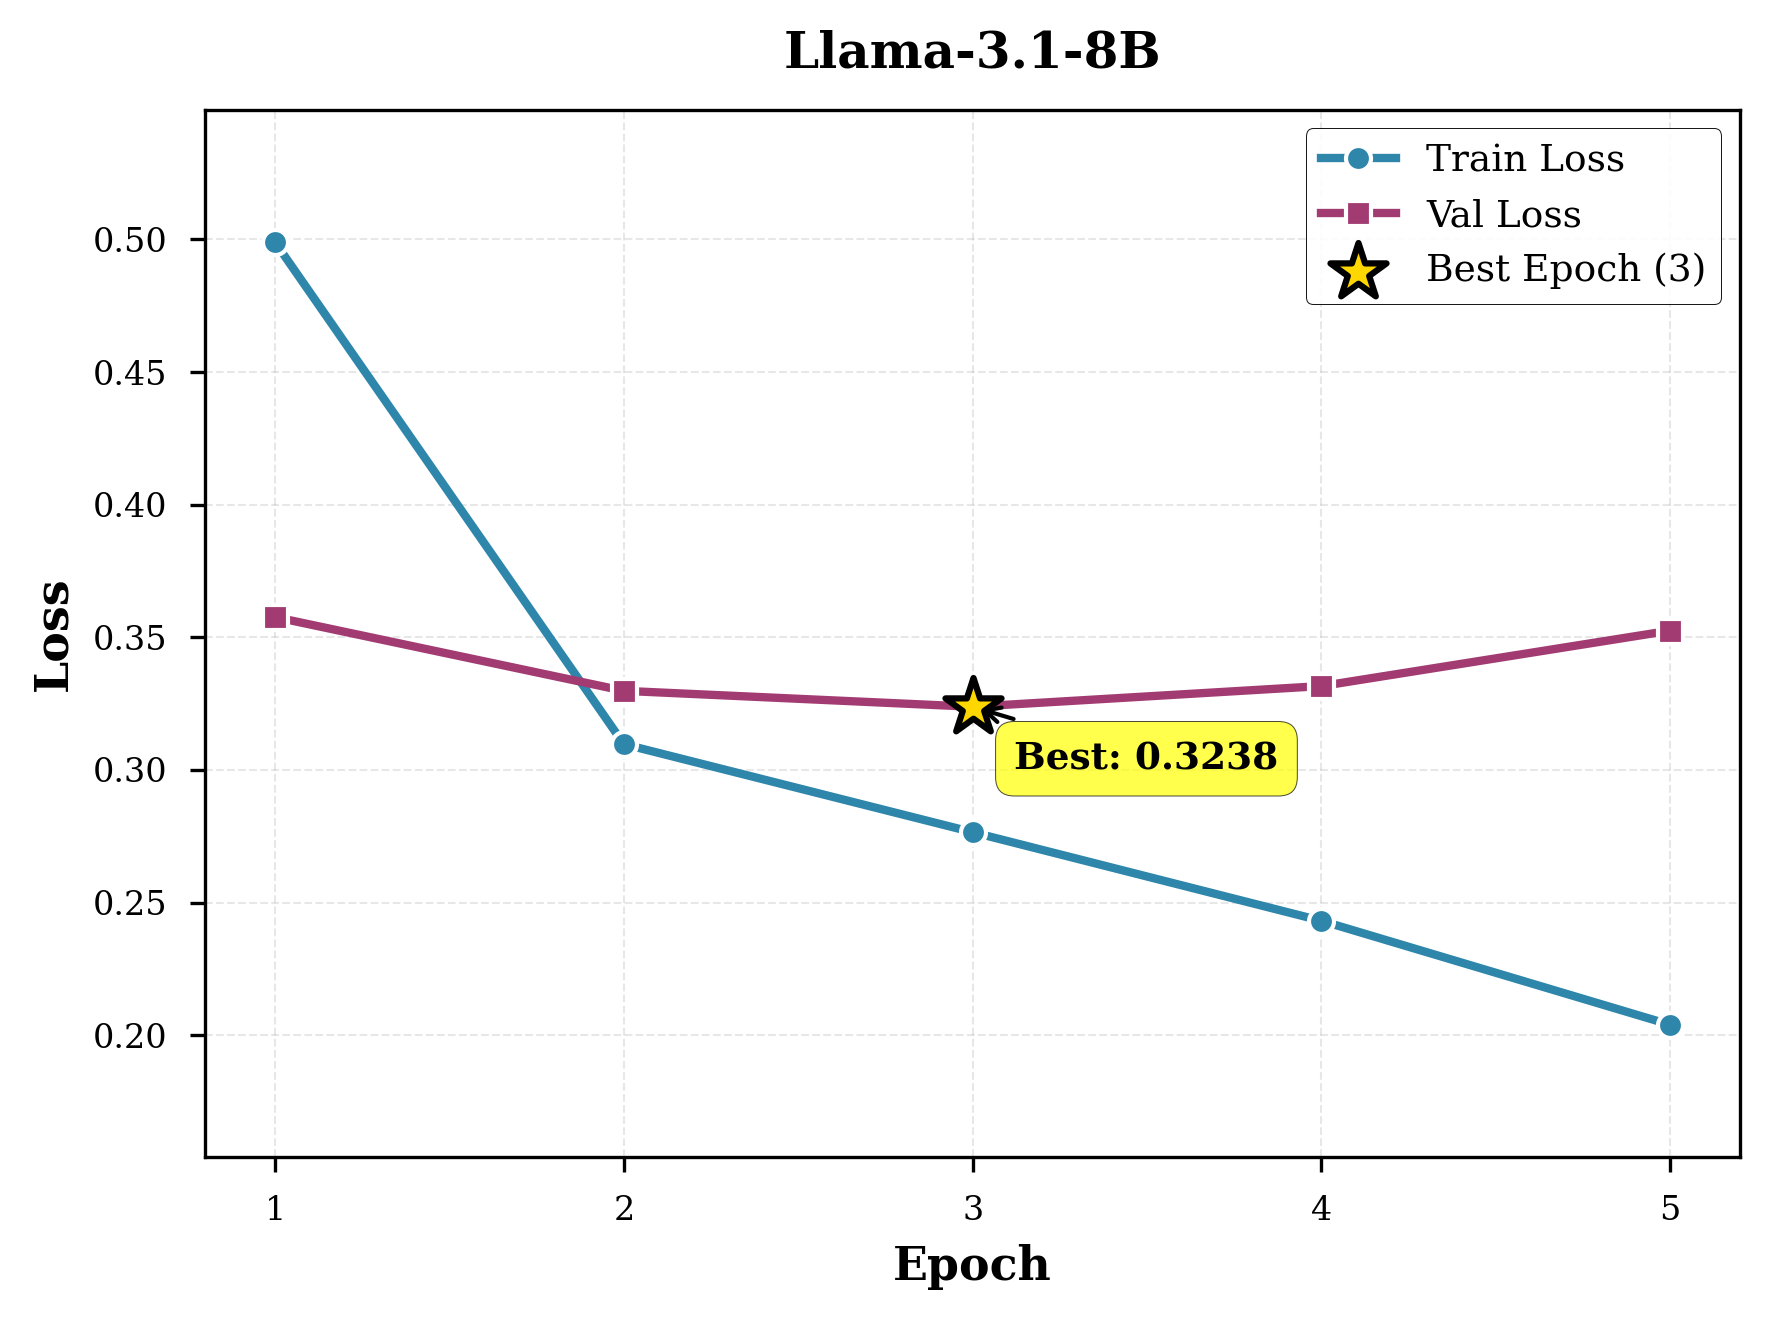
\includegraphics[width=\linewidth]{Images/training_curve_history_llama_31_8b.png}
        \caption{Textgen -- Llama-3.1-8B}
        \label{fig:task2-textgen-llama8b}
    \end{subfigure}\hfill
    \begin{subfigure}{0.5\textwidth}
        \centering
        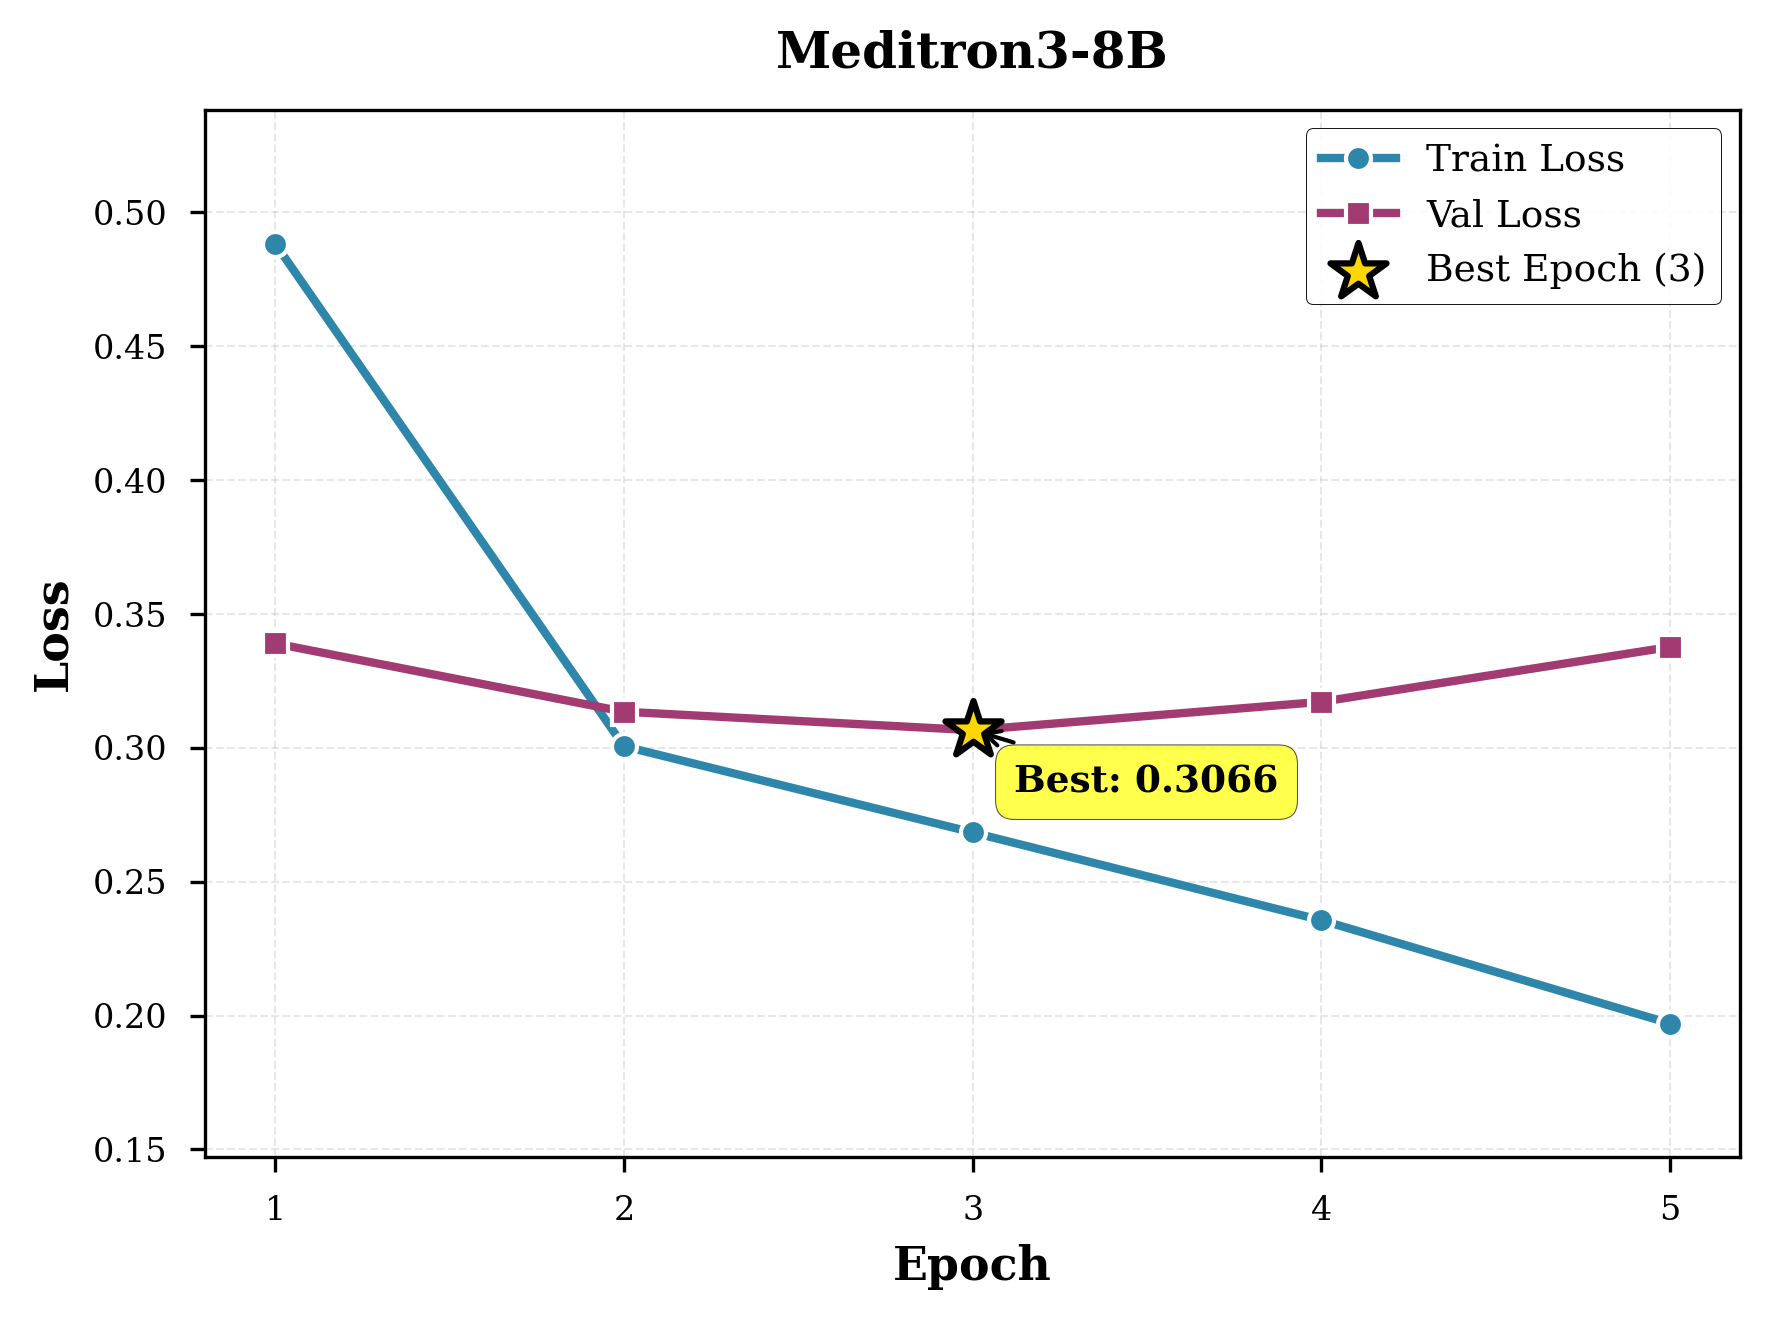
\includegraphics[width=\linewidth]{Images/training_curve_history_meditron3_8b.png}
        \caption{Textgen -- Meditron-8B}
        \label{fig:task2-textgen-meditron8b}
    \end{subfigure}
    \begin{subfigure}{0.5\textwidth}
        \centering
        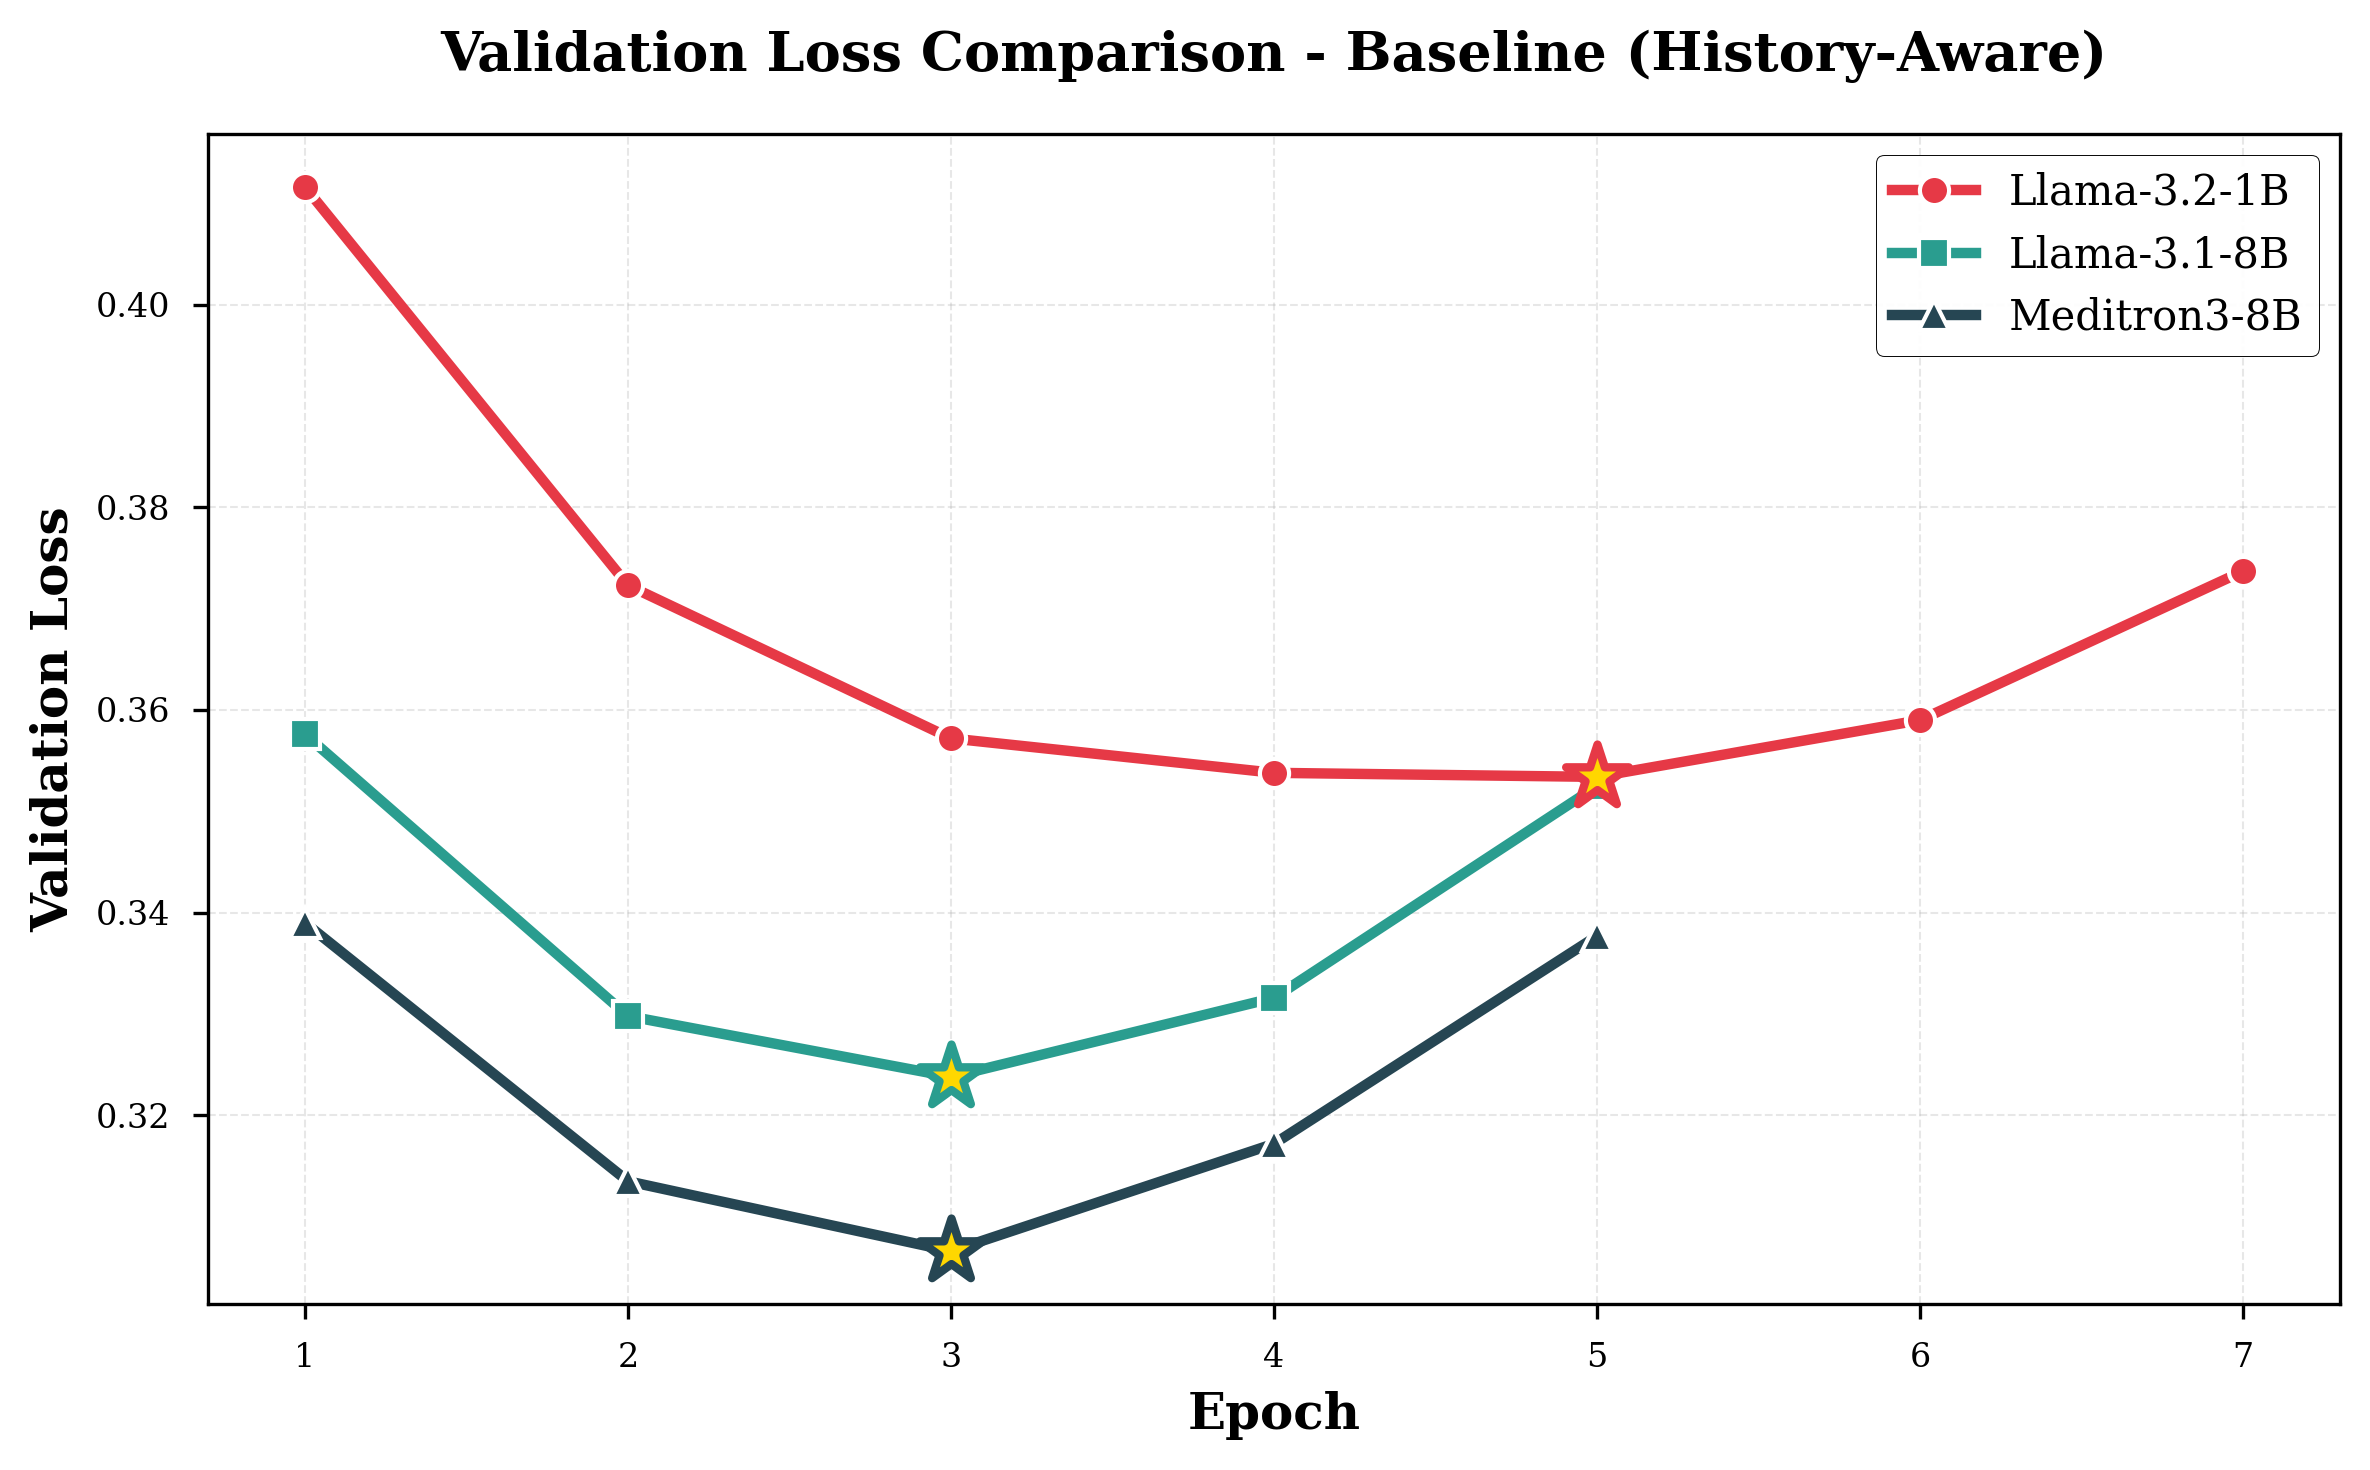
\includegraphics[width=\linewidth]{Images/validation_loss_comparison_history.png}
        \caption{Validation loss comparison}
        \label{fig:task2-textgen-val-loss-comparison}
    \end{subfigure}
    \caption{Task~2 (next-visit diagnosis prediction), Textgen pipeline. Training and validation loss across epochs for each backbone model.}
    \label{fig:task2-textgen-training}
\end{figure}

\paragraph{Distributed training and stability.}
All fine-tuning runs are performed in a multi-GPU setting (3) on NVIDIA H100 GPUs, using PyTorch Distributed Data Parallel (DDP) to scale training over long multimodal sequences. To ensure stability on shared infrastructure, we use conservative dataloader settings and explicit process-group cleanup at the end of training (synchronisation via barrier followed by teardown), reducing the risk of deadlocks or hangs during shutdown.

\paragraph{Inference configuration and output budget.}
At inference time, evaluation is executed on a single GPU using the best validation checkpoint. Codegen generates a continuation after a dedicated output marker and is explicitly instructed to output ICD-9-CM codes in canonical format; post-processing therefore only de-duplicates predictions and enforces the output budget. Textgen generates a list of diagnosis phrases, which are split into line-level candidates and mapped to ICD-9 codes via the ICD mapper (Section~\ref{subsec:textgen-arch}). Both the pipelines have to adhere to output budget tokens for fair comparison.

\paragraph{Token budgets and prompt packing.}
All runs use an explicit token-budgeting scheme to keep training and inference comparable across baselines and KG-augmented variants. We cap the \emph{base prompt} (structured context plus selected note sections, before injecting KG evidence) to \textbf{3072 tokens}. For KG-augmented prompts, we reserve an additional \textbf{1500-token} slot for linearised KG facts, followed by a \textbf{512-token} target budget for the assistant output, yielding a fixed \textbf{5120-token} total context window. For the \textbf{baseline} (no KG evidence), the same \textbf{3072-token} base-prompt cap and \textbf{512-token} target budget are used, and the remaining context window is left unused. This ensures fair comparison across all the experiments. When an example exceeds the available budget (e.g., long notes), the base prompt is truncated to fit the 3072-token cap using the same packing rule across all modes; KG evidence (when used) is then appended within its dedicated 1500-token slot.

% --------------------------------------------------------------------------------------------
\section{Knowledge Graph Integration}
\label{sec:kg-integration}

The clinical knowledge graph (KG) described in Section~\ref{subsec:kg-construction} is used to augment the neural baselines (Codegen and Textgen; Section~\ref{sec:model-architectures}) with structured biomedical knowledge. Rather than training a graph neural network jointly with the language model, the KG is exploited in a \emph{retrieval-augmented} fashion: medically meaningful paths between clinical concepts are pre-computed, embedded into a \emph{medical fact index}, and later retrieved as external knowledge during diagnosis prediction.

The overarching motivation is twofold. First, electronic health records are sparse and noisy, and many clinically relevant associations (e.g.\ risk factors, complications, drug--indication links) are only weakly expressed in any single admission. Ontology-level relations from UMLS and related vocabularies can compensate for this sparsity by connecting observed events to plausible diagnoses through curated biomedical edges~\cite{bodenreider2004umls}. Second, large language models (LLMs) are strong at reading and reasoning over natural language, but they do not natively enforce consistency with formal medical ontologies or code systems~\cite{shen2024ehrsurvey}. By converting KG paths into short textual ``facts'' and injecting them into the prompt, the model can consume symbolic knowledge in a form that is aligned with its pre-training.

The remainder of this section describes (i) how H1 and H2 KG paths are collected and indexed as medical facts, (ii) how these facts are retrieved using semantic and relation-weighted similarity, and (iii) how they are integrated into the Textgen pipeline via a RAG-style preprocessing step.


\subsection{From Heterogeneous Codes to CUI-Level Concept Sets}
\label{subsec:fact-index-cuis}

A central design choice in this work is to operate on \emph{UMLS Concept Unique Identifiers (CUIs)} rather than raw EHR codes. As discussed in Section~\ref{subsubsec:kg-mapping}, multiple vocabularies used in MIMIC-IV (ICD-9/10 for diagnoses, CPT and ICD-9-PCS for procedures, ATC/NDC for medications, and LOINC for laboratory tests) can all be mapped into the shared CUI space provided by UMLS~\cite{bodenreider2004umls}. This offers several advantages:

\begin{itemize}
    \item different codes that denote the same underlying concept (e.g.\ synonymous ICD-9 codes, NDC variants of the same drug) collapse to a single CUI, reducing artificial sparsity;
    \item relations in the KG are defined between CUIs, so code-level events can be connected through ontology edges without losing semantic alignment;
    \item the preferred terms and synonyms associated with each CUI can be reused as natural-language descriptions when verbalising KG paths.
\end{itemize}

For \textbf{Task~1}, we construct a global set of \emph{source concepts} by aggregating all structured codes observed across the full cohort: medications, procedures, and laboratory tests (and, optionally, concurrent diagnoses) are mapped to CUIs and deduplicated. For \textbf{Task~2}, this source set is extended to also include CUIs corresponding to \emph{past diagnoses} from previous visits, reflecting the longitudinal risk profile.

Independently, we form a set of \emph{target concepts} consisting of CUIs corresponding to all diagnosis codes used as labels in either task. These target CUIs represent the disease entities for which KG-based evidence will be collected. The medical fact index is then built from paths connecting this global source set to the diagnosis target set.


\subsection{Path Families H1 and H2 on the Global KG}
\label{subsec:fact-index-path-families}

On the global KG $\mathcal{G} = (\mathcal{V}, \mathcal{E})$ we define two families of clinically meaningful paths between source and target concepts. Let $\mathcal{S} \subset \mathcal{V}$ denote the set of source CUIs and $\mathcal{D} \subset \mathcal{V}$ the set of diagnosis CUIs.

\paragraph{H1: Direct source-to-diagnosis paths (1-hop).}

The first family, denoted $\mathcal{P}_{\text{H1}}(d)$ for a diagnosis $d \in \mathcal{D}$, consists of all \emph{1-hop} paths from any source concept $s \in \mathcal{S}$ to $d$:
\begin{equation}
    \mathcal{P}_{\text{H1}}(d)
    =
    \left\{ p = (s \xrightarrow{r} d) \;\middle|\; s \in \mathcal{S},\; (s,d) \in \mathcal{E} \right\},
\end{equation}
where $r$ is the canonical relation type (\texttt{rela\_canon}) associated with the edge (Section~\ref{subsubsec:kg-relations}).

These paths capture direct clinical relations such as
\begin{itemize}
    \item \texttt{ETIOLOGY\_OF} (\emph{``chronic kidney disease'' is an etiology of ``anaemia in chronic disease''}),
    \item \texttt{HAS\_COMPLICATION} (\emph{``diabetes mellitus'' has complication ``diabetic nephropathy''}), or
    \item \texttt{MAY\_TREAT} (\emph{``warfarin'' may treat ``atrial fibrillation''}).
\end{itemize}
They represent strong, local evidence that a diagnosis is mechanistically or therapeutically connected to an observed medication, procedure, lab, or history diagnosis.

\textcolor{red}{\textbf{[TODO: Insert example H1 subgraph]}}

\paragraph{H2: Indirect source-to-diagnosis paths (2-hop).}

The second family, denoted $\mathcal{P}_{\text{H2}}(d)$, consists of \emph{short multi-hop} paths (length $2$) from any $s \in \mathcal{S}$ to $d$ via a single intermediate concept $m$:
\begin{equation}
    \mathcal{P}_{\text{H2}}(d)
    =
    \left\{
        p = (s = v_0 \xrightarrow{r_1} v_1 \xrightarrow{r_2} v_2 = d)
        \;\middle|\;
        s \in \mathcal{S},\; v_1 \in \mathcal{V}
    \right\}.
\end{equation}

\textcolor{red}{\textbf{[TODO: Insert example H2 subgraph]}}

These paths capture mediated relationships where the connection between a source concept and a diagnosis is explained via intermediate concepts such as risk factors, mechanisms, or complications. For example:
\[
    \text{Diabetes mellitus}
    \xrightarrow{\texttt{HAS\_COMPLICATION}}
    \text{Chronic kidney disease}
    \xrightarrow{\texttt{HAS\_COMPLICATION}}
    \text{Hyperkalaemia}.
\]
H2 paths are typically more numerous and noisier than H1 paths but can provide valuable evidence when direct links are absent.

By construction, both H1 and H2 paths are \emph{patient-independent}: they describe generic biomedical relations between EHR-derived CUIs and diagnosis CUIs. This makes them suitable as reusable ``medical facts'' that can be retrieved for any admission matching similar patterns.

\subsection{Relation Canonicalisation and Weight Assignment}
\label{subsec:relation-weights}

Raw relations from UMLS and related ontologies are heterogeneous and fine-grained. In the subset of UMLS relations considered for this work, there are initially 384 distinct relation labels (\texttt{rela\_raw}) after merging across sources (Section~\ref{subsubsec:kg-relations}). Directly using all of these labels would make reasoning and retrieval noisy and difficult to interpret.

As described earlier, these 384 labels are first mapped to a compact set of 25 \emph{canonical} relation types (\texttt{rela\_canon}) using a combination of rule-based grouping and expert-guided consolidation. Building on this, each canonical relation type $r$ is assigned a diagnostic importance weight $w(r) \in [0.3, 3.0]$.

Weights are obtained via a semi-automatic procedure:

\begin{enumerate}
    \item All 384 raw relation labels and their textual descriptions are provided to a domain-specialised LLM, prompted to act as a clinical knowledge expert. The model is asked to (i) cluster the raw labels into essential clinical relation types and (ii) assign each canonical type a scalar weight under explicit guidelines.
    \item The weighting guidelines instruct the model to use higher scores for relations that are directly relevant to diagnosis and prognosis (e.g.\ ``causes'', ``indicates'', ``may\_treat'') and lower scores for structural or administrative relations (e.g.\ ``is\_a'', ``has\_location'', ``temporal''). Concretely, five tiers are defined (see Figure~\ref{fig:relation-weight-tiers}):
    \begin{itemize}
        \item Tier~1 (weight $\approx 3.0$): direct causal/diagnostic relations such as \texttt{ETIOLOGY\_OF}, \texttt{MAY\_CAUSE}, \texttt{PATHOLOGY\_OF};
        \item Tier~2 (2.0--2.5): strong clinical associations such as \texttt{MAY\_TREAT}, \texttt{FINDING\_SITE}, \texttt{CLINICAL\_COURSE}, \texttt{ASSOCIATED\_WITH};
        \item Tier~3 (1.0--1.5): moderate associations such as \texttt{LOCATION\_OF}, measurement and procedure-method relations;
        \item Tier~4 (0.5--0.8): structural relations such as \texttt{IS\_A}, \texttt{EQUIVALENT\_TO}, and meta-relations;
        \item Tier~5 (0.3--1.2): low diagnostic value or largely administrative relations such as temporal order, intent, priority, or device metadata.
    \end{itemize}
    \item The resulting mapping from canonical relation types to weights is manually reviewed for obvious inconsistencies and then fixed for all subsequent experiments.
\end{enumerate}

This process yields a set of clinically interpretable relation weights $w(r)$ that will later be combined with semantic similarity to favour KG paths that are both textually relevant and diagnostically meaningful.

\begin{figure}[t]
    \centering
    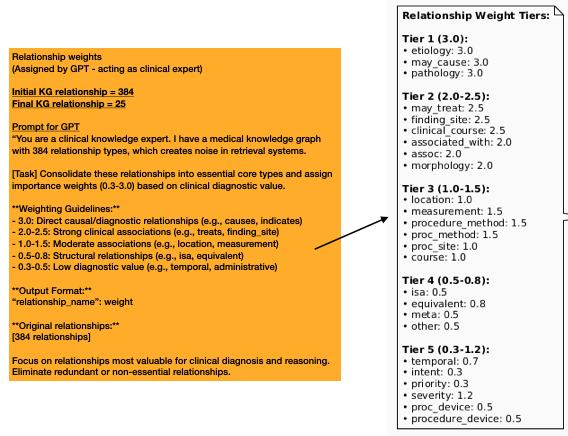
\includegraphics[width=\textwidth]{Images/RelationWeights.png}
    \caption{Schematic illustration of the relation-weight derivation. Left: prompt and weighting guidelines used to compress 384 raw KG relations into 25 canonical types. Right: example of the resulting tiered weight assignments, with higher weights reserved for etiologic, treatment, and complication relations.}
    \label{fig:relation-weight-tiers}
\end{figure}

For a specific path
\[
    p = (v_0 \xrightarrow{r_1} v_1 \xrightarrow{r_2} \dots \xrightarrow{r_L} v_L),
\]
we define a path-level KG score
\begin{equation}
    S_{\text{path}}(p)
    =
    \frac{1}{L} \sum_{\ell=1}^{L} w(r_\ell) \cdot \gamma^{\ell-1},
    \label{eq:path-score}
\end{equation}
where $\gamma \in (0,1]$ is a length discount factor that mildly penalises longer chains. For H1 paths ($L=1$), $S_{\text{path}}$ reduces to the weight of the single relation; for H2 paths, it averages the two relation weights with a small preference for edges closer to the diagnosis.

This scalar $S_{\text{path}}(p)$ is stored as metadata for each fact and later used in relation-weighted retrieval (Section~\ref{subsec:similarity-scoring}).

\subsection{Textual Linearisation and Semantic Encoding}
\label{subsec:fact-index-linearisation}

To interface with an LLM and with dense retrieval, each KG path must be represented in natural language. For each path $p \in \mathcal{P}_{\text{H1}} \cup \mathcal{P}_{\text{H2}}$, we therefore generate a short textual description by concatenating the CUI descriptions with a relation-specific template.

For a direct H1 path $s \xrightarrow{r} d$, statements of the form
\begin{itemize}
    \item ``\emph{\texttt{<source label>}} is used to treat \emph{\texttt{<diagnosis label>}}'' (for \texttt{MAY\_TREAT}),
    \item ``\emph{\texttt{<diagnosis label>}} is a complication of \emph{\texttt{<source label>}}'' (for \texttt{HAS\_COMPLICATION}),
    \item ``\emph{\texttt{<source label>}} is a type of \emph{\texttt{<diagnosis label>}}'' (for \texttt{IS\_A}),
\end{itemize}
are used. For H2 paths $s \xrightarrow{r_1} m \xrightarrow{r_2} d$, templates chain the intermediate concept into a single sentence, for example:
\begin{quote}
    ``\emph{Diabetes mellitus} can lead to \emph{chronic kidney disease}, which in turn can cause \emph{hyperkalaemia}.'' 
\end{quote}

This \emph{linearisation} serves two purposes. First, it turns each path into a short, self-contained text snippet that can be directly concatenated into the model prompt. Second, it allows us to embed paths with standard biomedical sentence encoders, ensuring that semantic similarity between clinical notes and path facts is computed in a shared representation space.

For semantic encoding we use a SapBERT-style biomedical text encoder~\cite{liu2020self}. SapBERT is pre-trained by aligning synonyms of the same CUI to nearby points in embedding space, which makes it particularly effective for representing ontology terms and their textual variants. This property is advantageous in our setting for two reasons:

\begin{enumerate}
    \item CUI descriptions from UMLS and label titles from ICD-9 often differ from the phrasing used in clinical notes; SapBERT bridges this gap by pulling conceptually equivalent phrases together.
    \item Linearised paths frequently contain multiple CUIs; SapBERT's entity-centric training encourages embeddings that still reflect the underlying biomedical concepts even when they appear in longer sentences.
\end{enumerate}

Each linearised H1 and H2 path is encoded into a fixed-dimensional vector. Two separate FAISS indices~\cite{johnson2019billion} are then constructed:

\begin{itemize}
    \item an \textbf{H1 fact index} containing embeddings and metadata for all direct (1-hop) path statements;
    \item an \textbf{H2 fact index} containing embeddings and metadata for all indirect (2-hop) path statements.
\end{itemize}

Separating H1 and H2 at the index level enables ablation experiments (H1-only, H2-only, or combined retrieval) and reflects the intuition that direct and mediated evidence may play different roles in different diagnostic scenarios.

Figure~\ref{fig:fact-index-building} summarises the fact-index construction process, from EHR codes and KG relations to SapBERT embeddings stored in H1/H2 indices.

\begin{figure}[t]
    \centering
    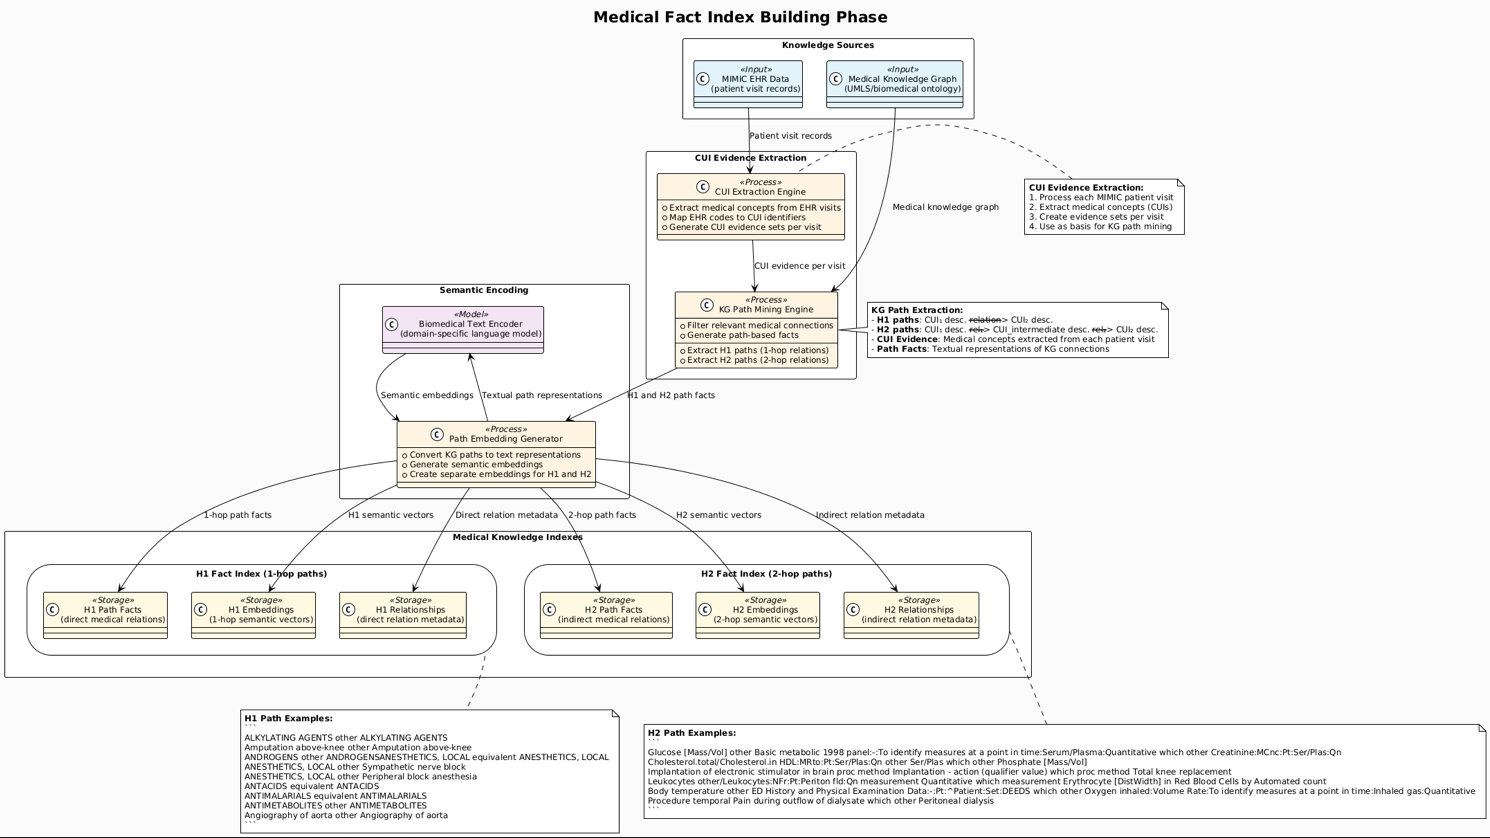
\includegraphics[width=\textwidth]{Images/MedicalFactIndex.png}
    \caption{Medical fact index building phase. Structured codes from MIMIC-IV are mapped to CUIs, H1/H2 KG paths are extracted between source and diagnosis CUIs, linearised into textual statements, encoded with a SapBERT biomedical encoder, and stored as separate H1/H2 semantic indices together with relation-derived metadata (e.g.\ canonical relation types and path scores).}
    \label{fig:fact-index-building}
\end{figure}

\subsection{RAG-Based Knowledge Injection for Textgen}
\label{subsec:kg-rag}

Once the H1 and H2 fact indices are built, they are used in a Retrieval-Augmented Generation (RAG) pipeline that enriches the Textgen prompts with KG-derived medical facts~\cite{lewis2020rag}. This process is applied during preprocessing for both training and evaluation.

\subsubsection{Clinical query formation}

For each admission, we form a \emph{clinical query} by taking the full set of selected note sections used in Textgen (Section~\ref{subsec:textgen-arch}): Chief Complaint, History of Present Illness, Past Medical History, Family History, Physical Exam, Pertinent Results, Brief Hospital Course (for Task~1 only), and Medications on Admission. Using the entire note rather than a hand-crafted summary has two key advantages:

\begin{itemize}
    \item it preserves subtle cues (e.g.\ symptom patterns, temporal phrases, comorbidities) that may match the KG paths in non-obvious ways; and
    \item it avoids introducing additional heuristic filters or extraction rules that could discard relevant information.
\end{itemize}

The clinical query text is encoded with the same SapBERT encoder used for the fact index, ensuring that notes and path statements live in the same embedding space.

\subsubsection{Retrieval of H1/H2 medical facts}

Given the query embedding, we perform nearest-neighbour search in the H1 and/or H2 FAISS indices. For each admission, we retrieve up to $K$ relevant path facts (in experiments, typically $K=50$) according to a similarity score. Two similarity computation schemes are considered (Section~\ref{subsec:similarity-scoring}), corresponding to an ``unweighted'' and a ``relation-weighted'' retrieval strategy.

The retrieved path statements, together with their metadata (H1/H2 flag, canonical relation types, path score $S_{\text{path}}$), form a compact, admission-specific knowledge set. As illustrated in Figure~\ref{fig:rag-preproc}, this knowledge is then concatenated with the existing multimodal prompt.

\begin{figure}[t]
    \centering
    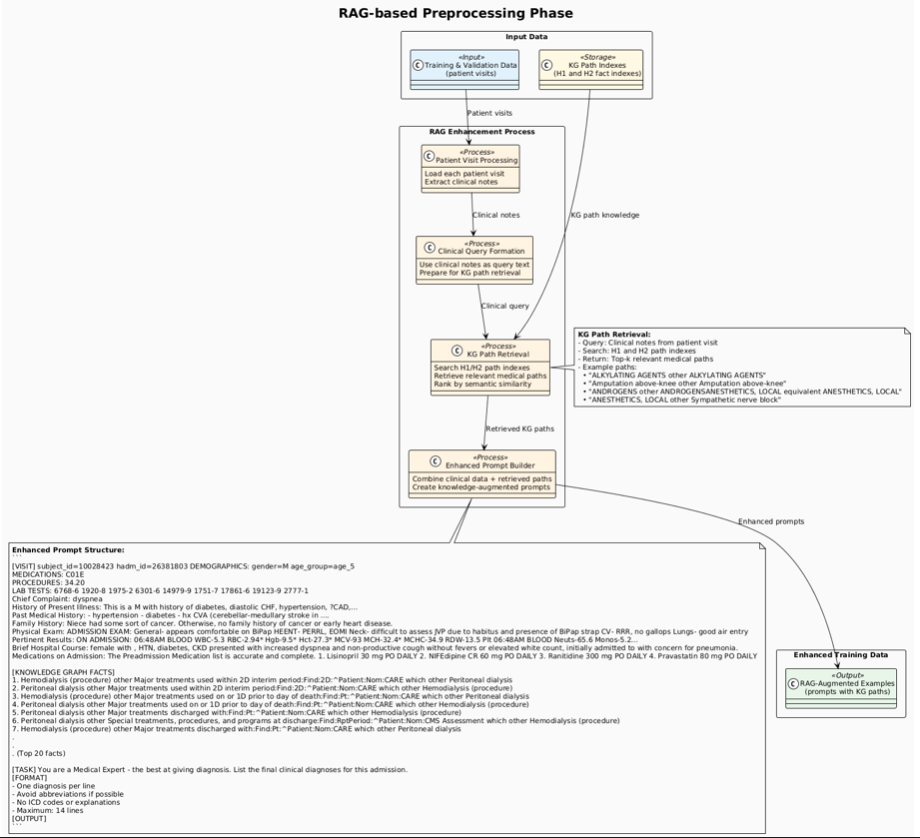
\includegraphics[width=\textwidth]{Images/RAG-based.png}
    \caption{RAG-based preprocessing phase. For each admission, the clinical note sections are encoded as a query, used to retrieve the top-$K$ relevant H1/H2 path facts from the KG indices, and combined with structured data to form a knowledge-augmented prompt for Textgen.}
    \label{fig:rag-preproc}
\end{figure}

\subsubsection{Knowledge-augmented prompts}

The retrieved path statements are appended to the Textgen prompt in a dedicated block, for example:

\begin{verbatim}
[KNOWLEDGE GRAPH FACTS]
1. Long-term diabetes mellitus can lead to chronic kidney disease.
2. Chronic kidney disease is a risk factor for hyperkalaemia.
3. ACE inhibitors are used to treat heart failure.
...
(Top 50 facts)
\end{verbatim}

\textcolor{red}{Include original facts here.}

An explicit header (e.g.\ \texttt{[KNOWLEDGE GRAPH FACTS]}) is used to clearly separate KG knowledge from patient-specific narrative. The task instructions in the prompt clarify that these items represent external medical knowledge that the model may use when deciding on final diagnoses, but that the predictions must remain consistent with the patient information.

This yields a \emph{Textgen+KG} variant in which the LLM jointly attends to structured codes, discharge summary, and KG-derived facts. No architectural changes to the Transformer are required; KG integration is realised entirely through the input context.

\subsubsection{Offline preprocessing vs.\ online retrieval}
\label{subsubsec:offline-online-rag}

The medical fact index is used in two complementary modes:

\begin{itemize}
    \item \textbf{Offline preprocessing for fine-tuning.} Before supervised fine-tuning, all training (and validation) admissions are passed through the RAG-based preprocessing pipeline (Figure~\ref{fig:rag-preproc}). For each admission, a clinical query is formed, the top-$K$ H1/H2 facts are retrieved once, and the resulting knowledge-augmented prompts are materialised to disk. Fine-tuning is then performed purely on these static, KG-augmented prompts. This avoids recomputing retrieval during every training epoch and ensures that the model sees a consistent set of KG facts for each example.

    \item \textbf{Online retrieval at inference time.} At inference, retrieval is performed \emph{on-the-fly}: the deployed system encodes the incoming clinical note, queries the H1/H2 indices, constructs a knowledge-augmented prompt for that particular visit, and feeds it to the fine-tuned Textgen model. This allows the KG evidence to reflect the most up-to-date medical fact index (e.g.\ after adding new paths or reweighting relations) without requiring the model to be retrained.
\end{itemize}

The separation between offline and online use of the fact index has practical benefits. Offline preprocessing keeps the fine-tuning pipeline simple and computationally efficient, while online retrieval makes the deployed system modular: the retriever, relation weights, or even the underlying KG can be updated independently of the language model, as long as the prompt format remains unchanged.

% \begin{figure}[t]
%     \centering
%     
\includegraphics[width=\textwidth]{Images/Empty.png}
%     \caption{Schematic comparison between offline KG-augmented training data preprocessing (left) and online retrieval with knowledge injection at inference time (right). The same H1/H2 medical fact indices are reused in both phases, but retrieval is performed once per example offline during fine-tuning and per-query online at deployment.}
%     \label{fig:offline-online-rag}
% \end{figure}

\textcolor{red}{Add the infographic for Online and Offline RAG here.}

This yields a \emph{Textgen+KG} variant in which the LLM jointly attends to structured codes, discharge summary, and KG-derived facts. No architectural changes to the Transformer are required; KG integration is realised entirely through the input context.

\subsection{Similarity Scoring: Unweighted vs.\ Relation-Weighted Retrieval}
\label{subsec:similarity-scoring}

\subsubsection{Unweighted semantic retrieval}

In the unweighted setting, retrieval is purely semantic. Let $q \in \mathbb{R}^d$ be the embedding of the clinical query, and $f_j \in \mathbb{R}^d$ the embedding of the $j$-th path fact in the index. The relevance score is given by the cosine similarity:
\begin{equation}
    s_{\text{sem}}(q, f_j)
    =
    \frac{\langle q, f_j \rangle}{\|q\| \, \|f_j\|}.
\end{equation}
The top-$K$ facts are selected according to $s_{\text{sem}}$, without explicit consideration of which relation types they instantiate. This corresponds to a standard dense-retrieval RAG pipeline~\cite{lewis2020rag} and serves as a strong baseline that tests whether purely semantic alignment between notes and KG paths is already beneficial.

\subsubsection{Relation-weighted retrieval}

While semantic similarity captures how well a path statement matches the language of the notes, it does not distinguish between highly informative relations (e.g.\ etiological or complication links) and weaker associations (e.g.\ vague ``associated with'' edges). The relation weights $w(r)$ and path scores $S_{\text{path}}(p)$ described in Section~\ref{subsec:relation-weights} provide a principled way to encode this additional diagnostic signal.

For each path fact $p$, we compute a normalised importance score
\begin{equation}
    \tilde{w}(p)
    =
    \frac{S_{\text{path}}(p) - \mu}{\sigma},
\end{equation}
where $\mu$ and $\sigma$ are the mean and standard deviation of $S_{\text{path}}$ across all facts in the index (or across a representative subset). The final relation-weighted relevance score is a convex combination of semantic similarity and normalised path importance:
\begin{equation}
    s_{\text{w}}(q, p)
    =
    \alpha \, s_{\text{sem}}(q, p)
    + (1 - \alpha) \, \tilde{w}(p),
    \label{eq:weighted-score}
\end{equation}
where $\alpha \in [0,1]$ controls the trade-off between semantic and symbolic evidence.

Intuitively, this scheme boosts KG facts that both \emph{match the note text} and \emph{instantiate clinically important relations}. For example, a path expressing that ``chest pain may cause myocardial infarction'' with a high etiological weight may be ranked above a semantically similar path that only expresses a non-specific association. Figure~\ref{fig:similarity-weighting} visualises the two retrieval strategies and illustrates how relation weights influence the final ranking.

\begin{figure}[t]
    \centering
    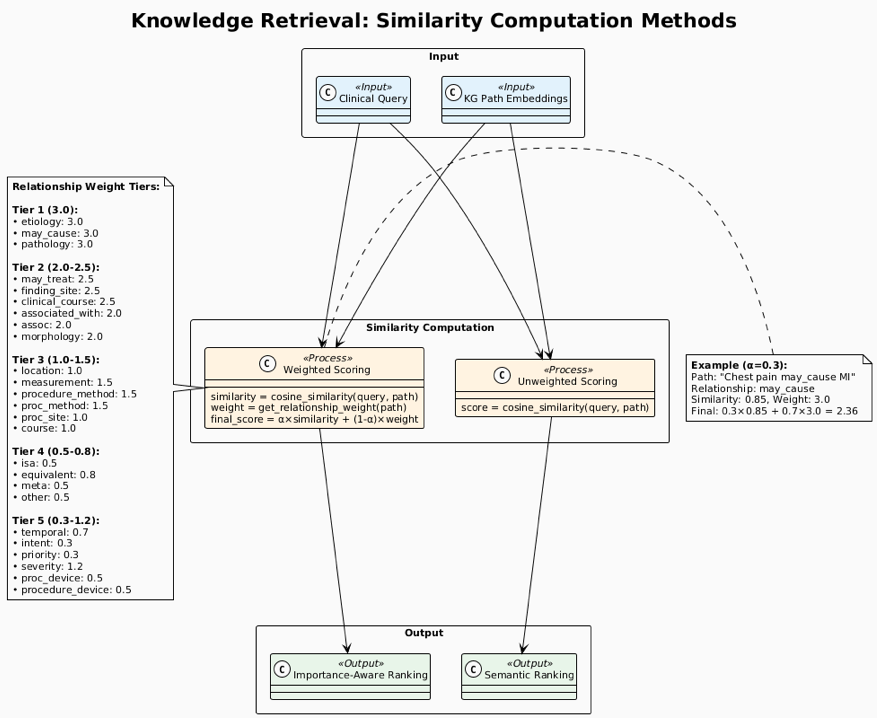
\includegraphics[width=\textwidth]{Images/KnowledgeRetrieval.png}
    \caption{Similarity computation methods. Right branch: unweighted retrieval uses only cosine similarity between the clinical query and path embeddings. Left branch: relation-weighted retrieval combines semantic similarity with a relation-tier weight derived from canonical KG relation types, favouring diagnostically informative paths.}
    \label{fig:similarity-weighting}
\end{figure}

\subsubsection{Task-specific variants and ablations}

Both similarity schemes are applied for Task~1 and Task~2. In Task~1, H1 evidence (direct drug--disease and test--disease links) is expected to be particularly influential, whereas Task~2 can benefit more from H2 chains that bridge historical diagnoses to future complications. The experimental chapter therefore compares the following variants:

\subsection{Interpretability of KG-Enhanced Predictions}
\label{subsec:kg-interpretability}

An additional benefit of the medical fact index is interpretability. For any predicted diagnosis, one can inspect the retrieved KG paths that are most relevant to the clinical notes. Because these paths are expressed in natural language and grounded in curated ontologies, they provide human-readable rationales linking observed findings and treatments to suggested diagnoses (e.g.\ ``Long-term diabetes mellitus can lead to chronic kidney disease, which in turn can cause hyperkalaemia'').

In this sense, the KG integration layer turns the base Textgen model into a neuro-symbolic predictor: the LLM proposes diagnoses based on multimodal inputs, and the KG contributes additional, ontology-grounded evidence via relation-aware retrieval. This aligns the proposed system with the broader trend towards explainable, knowledge-augmented clinical decision support~\cite{shang2019gamenet,choi2017gram}, where symbolic reasoning and neural models are combined to yield both accurate and interpretable predictions.



% \section{Knowledge Graph Integration}
% \label{sec:kg-integration}

% The clinical knowledge graph (KG) described in Section~\ref{subsec:kg-construction} is used to augment the neural baselines (Codegen and Textgen; Section~\ref{sec:model-architectures}) with structured biomedical knowledge. Instead of learning a graph neural network jointly with the language model, we integrate the KG in a \emph{retrieval-augmented} manner: clinically meaningful paths between concepts are pre-computed offline, verbalised into short natural-language statements (\emph{medical facts}), embedded into a semantic index, and later retrieved and injected into the prompt during diagnosis generation.

% The motivation is primarily methodological. EHR observations are heterogeneous (codes + narrative), while the KG provides an ontology-centric view over the same clinical concepts (Section~\ref{subsec:kg-construction}). By converting KG paths into compact textual facts, the system can (i) retrieve ontology-grounded relations that are relevant to the admission context and (ii) present them to the LLM in a form compatible with its language-model interface.

% Concretely, this section describes: (i) how cohort signals are mapped into CUI-level concept sets for retrieval, (ii) how one-hop (H1) and two-hop (H2) path families are extracted and indexed as reusable medical facts, (iii) how facts are retrieved using semantic similarity with an optional relation-weighted ranking, and (iv) how retrieved facts are injected under a fixed prompt budget.

% % ============================================================
% \subsection{From cohort signals to CUI-level query and target sets}
% \label{subsec:kg_cui_sets}

% KG integration operates in the UMLS Concept Unique Identifier (CUI) space to align heterogeneous vocabularies under a shared identifier system (Section~\ref{subsec:kg-mapping}). Given an admission, the \emph{patient context} is represented as a set of CUIs mapped from the structured cohort features (diagnoses/procedures/medications/labs, depending on the task), while the \emph{retrieval query} is formed from the leakage-controlled note sections used by Textgen (Section~\ref{sec:model-architectures}). Working at the CUI level has two practical benefits in this pipeline:
% (i) KG relations are defined between CUIs, allowing path extraction without code-system fragmentation, and
% (ii) preferred names/synonyms attached to CUIs can be reused both to verbalise KG facts and to provide concept descriptions when prompts require human-readable labels.

% We also define a global \emph{diagnosis target set} $\mathcal{D}$ as the CUIs corresponding to the retained ICD label space (Section~\ref{sec:preprocessing}). The fact index is built from paths that connect cohort-derived source concepts to these diagnosis targets.

% % ============================================================
% \subsection{Path families H1 and H2 on the global KG}
% \label{subsec:kg_path_families}

% Let the global KG be $\mathcal{G}=(\mathcal{V},\mathcal{E})$. Let $\mathcal{S}\subset\mathcal{V}$ denote the set of \emph{source} CUIs (mapped from cohort signals) and $\mathcal{D}\subset\mathcal{V}$ the set of \emph{diagnosis} CUIs (mapped from label ICD codes). We extract two short path families that connect $\mathcal{S}$ to $\mathcal{D}$:

% \paragraph{H1: direct (1-hop) paths.}
% H1 consists of all edges from a source concept $s\in\mathcal{S}$ directly to a diagnosis concept $d\in\mathcal{D}$:
% \begin{equation}
% \mathcal{P}_{\mathrm{H1}}(d)
% =
% \left\{
% (s \xrightarrow{r} d)\ \middle|\ s\in\mathcal{S},\ (s,d)\in\mathcal{E}
% \right\},
% \end{equation}
% where the edge label $r$ corresponds to the KG relationship type (\texttt{rela}; and its canonical form \texttt{rela\_canon} after mapping).

% \paragraph{H2: mediated (2-hop) paths.}
% H2 consists of paths of length two from $s$ to $d$ via an intermediate concept $m$:
% \begin{equation}
% \mathcal{P}_{\mathrm{H2}}(d)
% =
% \left\{
% (s \xrightarrow{r_1} m \xrightarrow{r_2} d)\ \middle|\ s\in\mathcal{S},\ m\in\mathcal{V},\ d\in\mathcal{D}
% \right\}.
% \end{equation}
% H2 paths expand the candidate evidence space by allowing a single bridging concept (e.g., mechanism, complication, finding-site, risk factor). In practice, H2 is substantially larger than H1 and requires explicit ranking and budgeting during injection (Section~\ref{subsec:kg_budgeting}).

% Importantly, both H1 and H2 paths are \emph{patient-independent}: they encode reusable biomedical relations between concepts. Patient conditioning is introduced later through retrieval, i.e., which subset of the global fact index is selected for a particular admission.

% % ============================================================
% \subsection{Relation canonicalisation and path scoring}
% \label{subsec:kg_relation_weighting}

% As described in Section~\ref{subsec:kg-construction}, the extracted KG relations are heterogeneous: in our subset there are initially 384 distinct relationship labels (\texttt{rela}). To make retrieval and analysis tractable, these are mapped to \textbf{25 canonical relation types} (\texttt{rela\_canon}) using rule-based grouping with manual review. Canonicalisation provides a compact, interpretable relation schema used consistently throughout the pipeline (fact construction, scoring, and analysis).

% To support relation-aware ranking, each canonical relation type $r$ is assigned a diagnostic-importance weight $w(r)$ (tiered scheme; Figure~\ref{fig:relation-weight-tiers}). For a path
% \[
% p = (v_0 \xrightarrow{r_1} v_1 \xrightarrow{r_2}\dots\xrightarrow{r_L} v_L),
% \]
% we compute a path-level score that aggregates relation importance while mildly discounting later hops:
% \begin{equation}
% S_{\text{path}}(p)
% =
% \frac{1}{L}\sum_{\ell=1}^{L} w(r_\ell)\cdot \gamma^{\ell-1},
% \label{eq:path_score}
% \end{equation}
% where $\gamma\in(0,1]$ is a length discount factor. This score is stored as metadata for each fact and can be used during retrieval (Section~\ref{subsec:kg_retrieval_scoring}).

% % ============================================================
% \subsection{Fact linearisation and semantic indexing}
% \label{subsec:kg_fact_index}

% To make KG evidence consumable by an LLM (and retrievable via dense similarity search), each H1/H2 path is converted into a short textual statement using CUI preferred labels and relation-specific templates. For example, H1 paths yield single-edge statements (source--relation--diagnosis), while H2 paths yield chained statements that include the intermediate concept.

% Each linearised statement is embedded with a biomedical sentence encoder (SapBERT; Section~\ref{subsec:textgen-arch}) and stored in a FAISS index together with metadata (source/target CUIs, relation types, and $S_{\text{path}}$). We maintain separate indices for H1 and H2 facts, enabling controlled ablations and reflecting the operational differences between direct and mediated evidence (Figure~\ref{fig:fact-index-building}).

% % ============================================================
% \subsection{Retrieval and ranking of KG facts}
% \label{subsec:kg_retrieval_scoring}

% At run time (training preprocessing and inference), we encode the admission’s clinical query (selected note sections) into an embedding $q$. Retrieval is performed by nearest-neighbour search over the H1 and/or H2 indices. We consider two ranking schemes:

% \paragraph{Unweighted semantic retrieval.}
% Facts are ranked purely by cosine similarity between the query embedding $q$ and a fact embedding $f$:
% \[
% s_{\text{sem}}(q,f)=\frac{\langle q,f\rangle}{\|q\|\|f\|}.
% \]
% This serves as the semantic baseline: the retriever selects facts whose verbalised text is most similar to the note content.

% \paragraph{Relation-weighted retrieval.}
% Semantic similarity does not distinguish between relation types (e.g., highly diagnostic relations vs.\ structural links). We therefore also evaluate a relation-aware ranking that combines semantic similarity with the path score in Eq.~\eqref{eq:path_score}. Let $\widetilde{S}_{\text{path}}(p)$ denote a normalised version of $S_{\text{path}}(p)$ (e.g., z-scoring over the index). The combined score is:
% \begin{equation}
% s_{\text{w}}(q,p)
% =
% \alpha\, s_{\text{sem}}(q,p)
% +
% (1-\alpha)\, \widetilde{S}_{\text{path}}(p),
% \label{eq:weighted_score}
% \end{equation}
% with $\alpha\in[0,1]$. Figure~\ref{fig:similarity-weighting} illustrates the difference between the two schemes.

% % ============================================================
% \subsection{Budgeted knowledge injection and H1--H2 packing behaviour}
% \label{subsec:kg_budgeting}

% Retrieved facts are appended to the Textgen prompt in a dedicated block (Figure~\ref{fig:rag-preproc}). Knowledge injection is constrained by the fixed token budgets described in Section~\ref{sec:training}: a reserved KG-fact slot is available, and if the retrieved fact list exceeds this slot, facts are truncated in ranked order (unweighted or weighted).

% Table~\ref{tab:kg_budget_coverage_task1} reports how often the KG-fact block fits within the reserved KG budget on Task~1 across all prompts ($N=53{,}561$). The contrast between H1 and H2 is operationally important: H1 facts fit substantially more often than H2 facts, reflecting the rapid growth in candidate evidence with increased hop depth. This motivates careful ranking under fixed budgets, and provides a concrete rationale for evaluating relation-weighted retrieval particularly in multi-hop settings.

% \begin{table}[t]
% \centering
% \caption{KG fact-budget coverage on Task~1 under the fixed KG-fact slot ($N=53{,}561$ prompts). ``Fits'' counts examples where the retrieved fact block fits without truncation.}
% \label{tab:kg_budget_coverage_task1}
% \small
% \setlength{\tabcolsep}{4pt}
% \renewcommand{\arraystretch}{1.15}
% \begin{tabularx}{\linewidth}{l >{\centering\arraybackslash}X >{\centering\arraybackslash}X}
% \toprule
% \textbf{Mode} & \textbf{Fits / $N$} & \textbf{Fit rate} \\
% \midrule
% H1 (unweighted) & 38{,}241 / 53{,}561 & 71.40\% \\
% H1 (weighted)   & 44{,}035 / 53{,}561 & 82.21\% \\
% \midrule
% H2 (unweighted) & 4{,}251 / 53{,}561  & 7.94\% \\
% H2 (weighted)   & 4{,}007 / 53{,}561  & 7.48\% \\
% \bottomrule
% \end{tabularx}
% \end{table}

% \paragraph{Offline preprocessing and online inference.}
% For fine-tuning, retrieval is performed offline once per example and the resulting KG-augmented prompts are materialised, ensuring deterministic evidence per sample across epochs. At inference time, retrieval is performed online per admission, allowing updates to the fact index or relation-weighting scheme without modifying the LLM, as long as the prompt format remains unchanged.

% --------------------------------------------------------------------------------------------
\section{Evaluation Setup}
\label{sec:evaluation}

This section details how diagnosis prediction performance is quantified for both tasks introduced in Section~\ref{sec:problem-formulation}. We briefly summarise the data partitions (reusing the cohort splits defined earlier), clarify the label space and target construction, and describe the multi-label and hierarchical metrics used in the experiments. The goal is to ensure that the Results chapter can be interpreted unambiguously, especially in light of the vocabulary pruning described in Section~\ref{subsec:struct-process}.

\subsection{Data Partitions (Summary)}
\label{subsec:evaluation-splits}

All experiments reuse the subject-wise train--validation--test splits defined in Section~\ref{subsec:cohort-split}. In particular:

\begin{itemize}
    \item Splits are created at the \texttt{subject\_id} level, so that all admissions for a given patient fall entirely into \emph{one} of the training, validation, or test sets. This prevents information leakage where the model could learn patient-specific patterns from training admissions and exploit them on held-out admissions of the same patient.
    \item Approximately 80\% of patients are allocated to the training set, 10\% to validation, and 10\% to testing.
    \item For the longitudinal cohort used in Task~2, the relative proportions of multi-visit (``chronic'') and single-visit (``cold start'') patients defined in Section~\ref{sec:preprocessing} are preserved across splits, so that the mixture of history-rich and no-history cases remains comparable between training and evaluation.
\end{itemize}

The \emph{same} partitions are used for all model variants (Codegen, Textgen, and Textgen+KG) and all backbones. Performance differences can therefore be attributed to architectural and training choices rather than to differences in data sampling.

\subsection{Label Space and Target Construction}
\label{subsec:label-space}

Diagnosis prediction is evaluated as a multi-label classification problem over a \emph{pruned} ICD-9 code vocabulary, aligned with the vocabulary pruning applied in Section~\ref{subsec:struct-process}.

\paragraph{Pruned diagnosis vocabulary.}

As discussed earlier, ICD-9 codes in MIMIC-IV follow an extreme long-tail distribution, with thousands of very rare codes that are poorly suited to data-driven learning and graph-based reasoning. To mitigate this, we restrict the evaluation label space to the most frequent part of the distribution:

\begin{itemize}
    \item The diagnosis vocabulary $\mathcal{C}$ is defined as the set of the \textbf{2{,}000 most frequent ICD-9 diagnosis codes} in the \emph{training} split after normalisation.
    \item Codes are consistently normalised to a canonical ICD-9 format, with decimal points in their standard positions, before computing frequencies and building $\mathcal{C}$.
    \item At evaluation time, both ground-truth and predicted codes are intersected with $\mathcal{C}$. Diagnosis codes outside the top--2000 are treated as out-of-scope for this thesis and are not included in the metrics.
\end{itemize}

Thus, when we report ``ICD-9 code-level'' metrics, these always refer to \emph{exact-code performance within the pruned 2{,}000-code vocabulary}, not across the full ICD-9-CM ontology. This choice aligns the label space with the pruned input vocabulary used in the models and avoids having results dominated by ultra-rare codes that are neither well supported statistically nor structurally well integrated in the KG.

\paragraph{Task-specific temporal semantics of labels.}

The temporal definition of the label set differs between Task~1 and Task~2:

\begin{itemize}
    \item For \textbf{Task~1 (current-visit coding)}, the label set for each admission consists of the ICD-9 diagnosis codes assigned at discharge from the index visit, intersected with $\mathcal{C}$.
    \item For \textbf{Task~2 (next-visit prediction)}, the label set for an index admission \(T_n\) is defined as the union of ICD-9 diagnosis codes assigned in \emph{subsequent} admissions for the same patient that occur within the chosen prediction window(s) (e.g.\ within 12 months), again intersected with $\mathcal{C}$.
\end{itemize}

Given a set of diagnosis codes associated with each sample, ground-truth labels and model predictions are represented as multi-hot vectors over $\mathcal{C}$:
\[
    \mathbf{y}^{(i)}, \hat{\mathbf{y}}^{(i)} \in \{0,1\}^{|\mathcal{C}|},
\]
where $y^{(i)}_c = 1$ indicates that code $c \in \mathcal{C}$ is present for sample $i$, and $\hat{y}^{(i)}_c = 1$ indicates that the model predicted code $c$ for the same sample. For Codegen, $\hat{\mathbf{y}}^{(i)}$ is constructed directly from the generated codes; for Textgen, it is constructed \emph{after} the semantic mapping of generated diagnosis phrases back to ICD-9 codes.

\subsection{Multi-Label Classification Metrics}
\label{subsec:ml-metrics}

Given ground-truth vectors $\mathbf{y}^{(i)}$ and predictions $\hat{\mathbf{y}}^{(i)}$ over the shared vocabulary $\mathcal{C}$, we compute standard multi-label metrics using widely used implementations such as those in scikit-learn~\cite{pedregosa2011scikit}. Let $\mathcal{S}$ denote the set of samples (admissions) in the evaluation split.

\paragraph{Micro-averaged precision, recall, and F1.}

Micro-averaged metrics are computed by aggregating true positives (TP), false positives (FP), and false negatives (FN) across all labels and samples:
\[
    \text{Precision}_{\text{micro}} =
    \frac{\sum_{i \in \mathcal{S}} \text{TP}^{(i)}}{\sum_{i \in \mathcal{S}} \text{TP}^{(i)} + \sum_{i \in \mathcal{S}} \text{FP}^{(i)}}, \quad
    \text{Recall}_{\text{micro}} =
    \frac{\sum_{i \in \mathcal{S}} \text{TP}^{(i)}}{\sum_{i \in \mathcal{S}} \text{TP}^{(i)} + \sum_{i \in \mathcal{S}} \text{FN}^{(i)}}.
\]
The micro-F1 score is the harmonic mean of these two. Because the micro metrics weight each \emph{code occurrence} equally, they emphasise performance on frequent diagnoses and reflect overall coding accuracy in a head-heavy label space. In this thesis, micro-F1 at the ICD-9 code level serves as the \emph{primary headline metric} when comparing models.

\paragraph{Macro-averaged precision, recall, and F1.}

Macro-averaged metrics are computed by treating each code $c \in \mathcal{C}$ as an independent binary classification task, computing per-code precision, recall, and F1, and averaging over all codes:
\[
    \text{F1}_{\text{macro}} = \frac{1}{|\mathcal{C}|} \sum_{c \in \mathcal{C}} \text{F1}_c.
\]
Unlike micro-averaging, macro-averaging weights all codes equally, regardless of frequency. Macro-F1 therefore highlights how well models handle less frequent diagnoses within the pruned vocabulary and exposes whether improvements are confined to common codes or translate across the label space.

\paragraph{Sample-averaged precision, recall, and F1.}

Sample-averaged metrics are computed at the admission level. For each sample $i$, the predicted and true diagnosis sets are compared to obtain sample-specific precision and recall; these values are then averaged across admissions. This perspective gives equal weight to each clinical case, irrespective of how many codes it carries, and is clinically intuitive in scenarios where every admission is considered a unit of decision support.

All three families of metrics (micro, macro, and sample-averaged) are computed on binarised predicted vectors. For generative models, the decoded list of candidate codes is first de-duplicated, normalised, intersected with $\mathcal{C}$, and converted to $\hat{\mathbf{y}}^{(i)}$ before metrics are computed. In the Results chapter, we additionally report precision@k and recall@k (e.g.\ $k=5,10$) for selected models to approximate settings in which clinicians only inspect the top few suggested diagnoses.

\subsection{Hierarchical and Parent-Level Metrics}
\label{subsec:hierarchical-metrics}

ICD-9 encodes a natural hierarchy in which three-digit categories correspond to broad diagnostic \emph{families}, and additional digits define increasingly specific subtypes. From a clinical standpoint, predicting the correct disease family but an incorrect subtype is typically less harmful than missing the family entirely. To capture this notion of ``near misses'', we compute additional metrics at the parent-category level.

Each ICD-9 code $c$ is mapped to its three-digit parent $\pi(c)$ (e.g.\ 428.0, 428.1 $\rightarrow$ 428). For each admission $i$, the true and predicted parent sets are defined as
\[
    P_{\text{true}}^{(i)} = \{\pi(c) : c \in \text{true codes}^{(i)}\}, \quad
    P_{\text{pred}}^{(i)} = \{\pi(c) : c \in \text{predicted codes}^{(i)}\}.
\]

On top of the code-level metrics, we report:

\begin{itemize}
    \item \textbf{Parent-level macro-F1:} both ground-truth and predicted codes are collapsed to their parent categories, and macro-averaged F1 is recomputed on this reduced label set. This metric measures how well the models recover the correct \emph{disease families}, ignoring within-family subtype distinctions.
    \item \textbf{Parent recall and partial matches:} for each admission, we compute the fraction of true parents in $P_{\text{true}}^{(i)}$ that are recovered by at least one predicted code (i.e.\ where $\pi(c_{\text{pred}}) \in P_{\text{true}}^{(i)}$). We additionally track cases in which the parent category is correct but the specific child code is wrong as ``partial matches''. This provides insight into whether errors arise from missing the overall diagnostic category or from mis-specifying the level of detail within an otherwise correct family.
\end{itemize}

Together, exact code-level metrics and parent-level hierarchical metrics provide a more clinically nuanced view of performance: the former quantify strict coding accuracy over the pruned label space, while the latter capture whether predictions are at least directionally consistent with the ground-truth disease families.

\subsection{Axes of Comparison and Reported Metrics}
\label{subsec:model-comparisons}

The evaluation protocol is designed to support three main axes of comparison:

\begin{enumerate}
    \item \textbf{Architecture:} Codegen vs.\ Textgen for Task~1, under a fixed label space and identical data splits.
    \item \textbf{Backbone:} Llama-3.2-1B vs.\ Llama-3.1-8B vs.\ Meditron-8B, to assess the importance of model capacity and medical-domain pre-training.
    \item \textbf{Knowledge Graph augmentation:} Textgen vs.\ Textgen+KG, with different retrieval strategies (H1 vs.\ H2 vs.\ H1+H2 and unweighted vs.\ relation-weighted retrieval) as described in Section~\ref{sec:kg-integration}.
\end{enumerate}

Unless explicitly stated otherwise, the main tables in the Results chapter report:

\begin{itemize}
    \item ICD-9 \emph{code-level} micro-F1 (primary headline metric),
    \item ICD-9 \emph{code-level} macro-F1, and
    \item ICD-9 \emph{parent-level} macro-F1.
\end{itemize}

Sample-averaged metrics, precision/recall@k, and partial-match analyses are included wherever they offer additional diagnostic value, with extended breakdowns deferred to the Appendix.

% --------------------------------------------------------------------------------------------

